%%%%%%%%%%%%%%%%%%%%%%%%%%%%%%%%%%%%%%%%%
% Masters/Doctoral Thesis 
% LaTeX Template
% Version 2.5 (27/8/17)
%
% This template was downloaded from:
% http://www.LaTeXTemplates.com
%
% Version 2.x major modifications by:
% Vel (vel@latextemplates.com)
%
% This template is based on a template by:
% Steve Gunn (http://users.ecs.soton.ac.uk/srg/softwaretools/document/templates/)
% Sunil Patel (http://www.sunilpatel.co.uk/thesis-template/)
%
% Template license:
% CC BY-NC-SA 3.0 (http://creativecommons.org/licenses/by-nc-sa/3.0/)
%
%%%%%%%%%%%%%%%%%%%%%%%%%%%%%%%%%%%%%%%%%

%----------------------------------------------------------------------------------------
%	PACKAGES AND OTHER DOCUMENT CONFIGURATIONS
%----------------------------------------------------------------------------------------

\documentclass[
11pt, % The default document font size, options: 10pt, 11pt, 12pt
oneside, % Two side (alternating margins) for binding by default, uncomment to switch to one side
english, % ngerman for German
singlespacing, % Single line spacing, alternatives: onehalfspacing or doublespacing
%draft, % Uncomment to enable draft mode (no pictures, no links, overfull hboxes indicated)
%nolistspacing, % If the document is onehalfspacing or doublespacing, uncomment this to set spacing in lists to single
%liststotoc, % Uncomment to add the list of figures/tables/etc to the table of contents
%toctotoc, % Uncomment to add the main table of contents to the table of contents
%parskip, % Uncomment to add space between paragraphs
%nohyperref, % Uncomment to not load the hyperref package
headsepline, % Uncomment to get a line under the header
%chapterinoneline, % Uncomment to place the chapter title next to the number on one line
%consistentlayout, % Uncomment to change the layout of the declaration, abstract and acknowledgements pages to match the default layout
]{MastersDoctoralThesis} % The class file specifying the document structure

\usepackage[utf8]{inputenc} % Required for inputting international characters
\usepackage[T1]{fontenc} % Output font encoding for international characters

\usepackage{mathpazo} % Use the Palatino font by default

\usepackage[backend=bibtex,style=authoryear,natbib=true]{biblatex} % Use the bibtex backend with the authoryear citation style (which resembles APA)

\addbibresource{example.bib} % The filename of the bibliography

\usepackage[autostyle=true]{csquotes} % Required to generate language-dependent quotes in the bibliography

%----------------------------------------------------------------------------------------
%	MARGIN SETTINGS
%----------------------------------------------------------------------------------------

\geometry{
	paper=a4paper, % Change to letterpaper for US letter
	inner=2.5cm, % Inner margin
	outer=3.8cm, % Outer margin
	bindingoffset=.5cm, % Binding offset
	top=1.5cm, % Top margin
	bottom=1.5cm, % Bottom margin
	%showframe, % Uncomment to show how the type block is set on the page
}

%----------------------------------------------------------------------------------------
%	THESIS INFORMATION
%----------------------------------------------------------------------------------------

\thesistitle{Nonlinear finite element approach for contact problems in hyper-elastic models} % Your thesis title, this is used in the title and abstract, print it elsewhere with \ttitle
\supervisor{Dr. Nguyen Thanh \textsc{Nha}} % Your supervisor's name, this is used in the title page, print it elsewhere with \supname
\examiner{} % Your examiner's name, this is not currently used anywhere in the template, print it elsewhere with \examname
\degree{Student of Engineering Mechanics} % Your degree name, this is used in the title page and abstract, print it elsewhere with \degreename
\author{Nguyen Nhu Buu \textsc{duc}  Nguyen Ho Duy \textsc{tan}} % Your name, this is used in the title page and abstract, print it elsewhere with \authorname
\addresses{TP.HCM} % Your address, this is not currently used anywhere in the template, print it elsewhere with \addressname

\subject{Biological Sciences} % Your subject area, this is not currently used anywhere in the template, print it elsewhere with \subjectname
\keywords{} % Keywords for your thesis, this is not currently used anywhere in the template, print it elsewhere with \keywordnames
\university{\href{https://www.hcmut.edu.vn}{ho chi minh university of technology}} % Your university's name and URL, this is used in the title page and abstract, print it elsewhere with \univname
\department{\href{http://www.aao.hcmut.edu.vn/index.php?route=catalog/nganh&hedaotao_id=9&khoa_id=18&nganh_id=18}{Department of Engineering Mechanics}} % Your department's name and URL, this is used in the title page and abstract, print it elsewhere with \deptname
\group{\href{}{Research Group Name}} % Your research group's name and URL, this is used in the title page, print it elsewhere with \groupname
\faculty{\href{}{Faculty of Applied Science}} % Your faculty's name and URL, this is used in the title page and abstract, print it elsewhere with \facname

\AtBeginDocument{
\hypersetup{pdftitle=\ttitle} % Set the PDF's title to your title
\hypersetup{pdfauthor=\authorname} % Set the PDF's author to your name
\hypersetup{pdfkeywords=\keywordnames} % Set the PDF's keywords to your keywords
}

\begin{document}

\frontmatter % Use roman page numbering style (i, ii, iii, iv...) for the pre-content pages

\pagestyle{plain} % Default to the plain heading style until the thesis style is called for the body content

%----------------------------------------------------------------------------------------
%	TITLE PAGE
%----------------------------------------------------------------------------------------

\begin{titlepage}
    \begin{center}
    
    \vspace*{.06\textheight}
    {\scshape\LARGE \univname\par}\vspace{1.5cm} % University name
    \textsc{\Large graduate thesis}\\[0.5cm] % Thesis type
    
    \HRule \\[0.4cm] % Horizontal line
    {\huge \bfseries \ttitle\par}\vspace{0.4cm} % Thesis title
    \HRule \\[1.5cm] % Horizontal line
     
    \begin{minipage}[t]{0.4\textwidth}
        \begin{flushleft} \large
        \emph{Author:}\\
        \href{http://www.johnsmith.com}{\authorname} % Author name - remove the \href bracket to remove the link
        \end{flushleft}
        \end{minipage}
        \begin{minipage}[t]{0.4\textwidth}
        \begin{flushright} \large
        \emph{Supervisor:} \\
        \href{http://www.jamessmith.com}{\supname} % Supervisor name - remove the \href bracket to remove the link  
        \end{flushright}
    \end{minipage}\\[3cm]
     
    \vfill
    
    \large \textit{A thesis submitted in fulfillment of the requirements\\ for the degree of \degreename}\\[0.3cm] % University requirement text
    \textit{in the}\\[0.4cm]
    \groupname\\\deptname\\[2cm] % Research group name and department name
     
    \vfill
    
    {\large \today}\\[4cm] % Date
    %\includegraphics{Logo} % University/department logo - uncomment to place it
     
    \vfill
    \end{center}
    \end{titlepage}

%----------------------------------------------------------------------------------------
%	DECLARATION PAGE
%----------------------------------------------------------------------------------------
% 
\begin{declaration}
\addchaptertocentry{\authorshipname} % Add the declaration to the table of contents
\noindent I, \authorname, declare that this thesis titled, \enquote{\ttitle} and the work presented in it are my own. I confirm that:

\begin{itemize} 
\item This work was done wholly or mainly while in candidature for a research degree at this University.
\item Where any part of this thesis has previously been submitted for a degree or any other qualification at this University or any other institution, this has been clearly stated.
\item Where I have consulted the published work of others, this is always clearly attributed.
\item Where I have quoted from the work of others, the source is always given. With the exception of such quotations, this thesis is entirely my own work.
\item I have acknowledged all main sources of help.
\item Where the thesis is based on work done by myself jointly with others, I have made clear exactly what was done by others and what I have contributed myself.\\
\end{itemize}
 
\noindent Signed:\\
\rule[0.5em]{25em}{0.5pt} % This prints a line for the signature
 
\noindent Date:\\
\rule[0.5em]{25em}{0.5pt} % This prints a line to write the date
\end{declaration}

\cleardoublepage

%----------------------------------------------------------------------------------------
%	QUOTATION PAGE
%----------------------------------------------------------------------------------------

\vspace*{0.2\textheight}

\noindent\enquote{\itshape Thanks to my solid academic training, today I can write hundreds of words on virtually any topic without possessing a shred of information, which is how I got a good job in  journalism.}\bigbreak

\hfill Dave Barry

%----------------------------------------------------------------------------------------
%	ABSTRACT PAGE
%----------------------------------------------------------------------------------------
\chapter*{\centering Abstract}% Publications page text

Rubber, plastic, their similar materials and many other polymer materials are hyper elastic materials. We can see the use of these materials increasingly common in engineering with familiar products such as tires, car front-end covers, products made of plastic and rubber, etc. So solving the problems of hyper-elastic materials is essential in engineering. Solving these problems is a difficult engineering task. Since hyper-elastic materials have a stress-and-strain relationship that is nonlinear. Therefore, a suitable and effective method is required. And one of the most commonly used methods in engineering is the finite element method (FEM). . This paper discusses solving the contact problem between two elastic materials. In addition to using FEM, we also use high-order elements to deal with advantages such as: less element usage, more accurate results, geometrical flexibility....The contribution of the paper is that Matlab programs can calculate and simulate the specific contact problem between two hyper-elastic materials. To increase reliability, the obtained results are verified with the solutions given by FEA program. In summary, this paper said that it is high feasibility to use high-order elements in computational programming. With its advantages, the high-order elements are used in many contact problems requiring high accuracy. 

%----------------------------------------------------------------------------------------
%	ACKNOWLEDGEMENTS
%----------------------------------------------------------------------------------------

\begin{acknowledgements}
    \addchaptertocentry{\acknowledgementname} % Add the acknowledgements to the table of contents
    We would like to thank my supervisor, Dr. Nguyen Thanh Nha, for his enthusiastic support
during the past time. I would like to thank teachers in Department of Engineering
Mechanics, Faculty of Applied Science, Ho Chi Minh City University of Technology for
the knowledge and advices they have given to me for four years in college. This strong
basic helped me so much in the process of studying and completing this thesis.

    \end{acknowledgements}

%----------------------------------------------------------------------------------------
%	LIST OF CONTENTS/FIGURES/TABLES PAGES
%----------------------------------------------------------------------------------------

\tableofcontents % Prints the main table of contents

\listoffigures % Prints the list of figures

\listoftables % Prints the list of tables

%----------------------------------------------------------------------------------------
%	ABBREVIATIONS
%----------------------------------------------------------------------------------------

\begin{abbreviations}{ll} % Include a list of abbreviations (a table of two columns)

    \textbf{LAH} & \textbf{L}ist \textbf{A}bbreviations \textbf{H}ere\\
    \textbf{WSF} & \textbf{W}hat (it) \textbf{S}tands \textbf{F}or\\
    
    \end{abbreviations}

%----------------------------------------------------------------------------------------
%	PHYSICAL CONSTANTS/OTHER DEFINITIONS
%----------------------------------------------------------------------------------------

\begin{constants}{lr@{${}={}$}l} % The list of physical constants is a three column table

    % The \SI{}{} command is provided by the siunitx package, see its documentation for instructions on how to use it
    
    Speed of Light & $c_{0}$ & \SI{2.99792458e8}{\meter\per\second} (exact)\\
    %Constant Name & $Symbol$ & $Constant Value$ with units\\
    
    \end{constants}
    
%----------------------------------------------------------------------------------------
%	SYMBOLS
%----------------------------------------------------------------------------------------

\begin{symbols}{lll} % Include a list of Symbols (a three column table)

    % $a$ & distance & \si{\meter} \\
    % $P$ & power & \si{\watt} (\si{\joule\per\second}) \\
    % %Symbol & Name & Unit \\
    
    % \addlinespace % Gap to separate the Roman symbols from the Greek
    
    % $\omega$ & angular frequency & \si{\radian} \\
   

    $\{u\}$ & Displacement vector\\
    $\{\varepsilon\}$ & Strain vector\\
    $[D]$ & Differentiation operation matrix\\
    $\{\sigma\}$ & Stress vector\\
    $[E]$ & Elasticity matrix\\
    $\lambda,\mu$ & Lame constants\\
    $v$ & Poisson’s ratio\\
    $\Pi$ & Total potential \\
    $\{p^v\}$ & Body force vector\\
    $\{p^s\}$ & Surface force vector\\
    $\{q\}$ & Nodal displacement vector\\
    $[N]$ & Shape function matrix\\
    $[B]$ & Displacement differentiation matrix\\
    $[K]$ & Element stiffness matrix\\
    $\{f\}$ & Load vector\\
    $\{p\}$ & Actual forces vector\\
    $\{h\}$ & Thermal vector\\

    \end{symbols}
    

%----------------------------------------------------------------------------------------
%	DEDICATION
%----------------------------------------------------------------------------------------

\dedicatory{For my Family\ldots} 

%----------------------------------------------------------------------------------------
%	THESIS CONTENT - CHAPTERS
%----------------------------------------------------------------------------------------

\mainmatter % Begin numeric (1,2,3...) page numbering

\pagestyle{thesis} % Return the page headers back to the "thesis" style

% Include the chapters of the thesis as separate files from the Chapters folder
% Uncomment the lines as you write the chapters

% Chapter 1

\chapter{Introduction} % Main chapter title

\label{Chapter1} % For referencing the chapter elsewhere, use \ref{Chapter1} 

%----------------------------------------------------------------------------------------

% Define some commands to keep the formatting separated from the content 
\newcommand{\keyword}[1]{\textbf{#1}}
\newcommand{\tabhead}[1]{\textbf{#1}}
\newcommand{\code}[1]{\texttt{#1}}
\newcommand{\file}[1]{\texttt{\bfseries#1}}
\newcommand{\option}[1]{\texttt{\itshape#1}}

%----------------------------------------------------------------------------------------

\section{Introduction of Contact problems}
The contact problems are very importance in industrial applications in mechanical and civil engineering. The range of application are profusely such as metal forming processes, drilling problems, bearings or crash analysis of cars. Other applications are related to biomechanics where human joints, implant or teeth are considered. Due to this variety contact problems are today combined either with large elastic or inelastic deformations
including time dependent responses. Thermal coupling might have to be considered, see the cooling of electronic devices, the heat removal within nuclear power plant vessels or
thermal insulation of astronautic vehicles. Even stability behavior has to be linked tocontact, like wrinkling arising in metal forming problems. \parencite{ref1} Due to this technical importance a great number of researchers have investigated contact
problems. Starting with the classical analytical work of Hertz (1882) on the elastic contact of two spheres the deformation of the bodies being in contact has been taken into account. However only very few problems involving contact can be solved analytically. Thus for
most industrial applications numerical methods have to be applied when the contacting bodies have complex geometries . Due to that the solution of contact problems with finite
element methods has a relatively long history. \parencite{ref1}
The following introductory remarks are related to the steps which have to be followed when
treating contact problems within the finite element method. \parencite{ref1}


%----------------------------------------------------------------------------------------

\section{ Introduction of Hyper-elastic materials}
Hyper-elastic materials are designed for modeling rubber or rubber-like materials in which the elastic deformation can be extremely large. 

\begin{figure}[H]
    \centering
    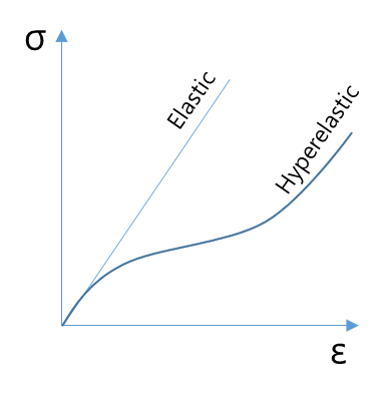
\includegraphics[scale=1]{Figures/Hyperelastic.png}
    \decoRule   
    \caption{ Introduction of hyper-elastic materials.}
    \label{fig:Electron}
\end{figure}
Hyper-elastic materials use something called a strain energy density function to derive the relationship between stress and strain. This allows them to model the relationship between stress and strain accurately even when the strain is between 100 \% to 700 \%, depending on the exact hyper-elastic model that is used.
Various hyper-elastic models are accurate over different range of strains. You must choose the model to use depending on the expected range of strains, the computational expense of the formulation and the amount of data that you have to define in the stress-strain relationship.

\section{Study objective}
In this study, contact problems with hyper-elastic materials will be considered in cases of frictionless sliding and frictionless compressing and the obtained results will be verified with the solution given by commercial program. From the theories and algorithms about contact problems and hyper – elastics materials based on finite element method, some
programs have to be made to resolve the problem of contact for hyper – elastic materials. These example will be programmed by using MATLAB and Python programming
languages, then the results which will be obtained from these programs will be compared to the results of commercial program (ANSYS).



%\chapter{ FEM - Theoretical Foundations and Applications } % Main chapter title

\label{Chapter2 } % For referencing the chapter elsewhere, use \ref{Chapter1} 
% \setlength{\parskip}{0.38cm}

%----------------------------------------------------------------------------------------

\section{Elasticity theory and applications \parencite{ref5}}
Theory of Elasticity presents the theory of stress, deformation and displacement analysis in elastic bodies of different shapes, It is subjected to external causes such as loads, temperature changes, etc. .
%----------------------------------------------------------------------------------------
\section{Solution of the problem of elasticity theory \parencite{ref5} }\label{theory}
In this section, we discuss elastic theoretical equations help to establish the problem.

\begin{itemize}
\item 3 equilibrium equations
    \begin{equation}
        \begin{split}
        \frac{{\partial {\sigma _x}}}{{\partial x}} + \frac{{\partial {\tau _{yx}}}}{{\partial y}} + \frac{{\partial {\tau _{zx}}}}{{\partial z}} + X = 0\\
        \frac{{\partial {\tau _{xy}}}}{{\partial x}} + \frac{{\partial {\sigma _y}}}{{\partial y}} + \frac{{\partial {\tau _{zy}}}}{{\partial z}} + Y = 0\\
        \frac{{\partial {t_{xz}}}}{{\partial x}} + \frac{{\partial {\tau _{yz}}}}{{\partial y}} + \frac{{\partial {\sigma _z}}}{{\partial z}} + Z = 0
        \end{split}
    \end{equation}
\item 6 deformation equations
\begin{list}{+}{}
    \item By Cauchy:
        \begin{equation}
    \begin{split}
        {{\varepsilon _x} = \frac{{\partial u}}{{\partial x}}; \qquad}&{{y_{xy}} = \frac{{\partial u}}{{\partial y}} + \frac{{\partial v}}{{\partial x}}}\\
        {{\varepsilon _y} = \frac{{\partial v}}{{\partial y}}; \qquad}&{{y_{yz}} = \frac{{\partial v}}{{\partial z}} + \frac{{\partial w}}{{\partial y}}}\\
        {{\varepsilon _z} = \frac{{\partial w}}{{\partial z}}; \qquad}&{{y_{zx}} = \frac{{\partial w}}{{\partial x}} + \frac{{\partial u}}{{\partial z}}}
    \end{split}
    \end{equation}
    \item By Saint-Venant:
    \begin{equation}
        \begin{gathered}
\frac{{{\partial ^2}{\gamma _{xy}}}}{{\partial x\partial y}} = \frac{{{\partial ^2}{\varepsilon _x}}}{{\partial {y^2}}} + \frac{{{\partial ^2}{\varepsilon _y}}}{{\partial {x^2}}}\\
\frac{{{\partial ^2}{y_{yz}}}}{{\partial y\partial z}} = \frac{{{\partial ^2}{\varepsilon _y}}}{{\partial {z^2}}} + \frac{{{\partial ^2}{\varepsilon _z}}}{{\partial {y^2}}}\\
\frac{{{\partial ^2}{y_{zx}}}}{{\partial z\partial x}} = \frac{{{\partial ^2}{\varepsilon _z}}}{{\partial {x^2}}} + \frac{{{\partial ^2}{\varepsilon _x}}}{{\partial {z^2}}}\\
2\frac{{{\partial ^2}{\varepsilon _x}}}{{\partial y\partial z}} = \frac{\partial }{{\partial x}}\left( {\frac{{ - \partial {y_{yz}}}}{{\partial x}} + \frac{{\partial {\gamma _{zx}}}}{{\partial y}} + \frac{{\partial {\gamma _{xy}}}}{{\partial z}}} \right)\\
2\frac{{{\partial ^2}{\varepsilon _y}}}{{\partial z\partial x}} = \frac{\partial }{{\partial y}}\left( {\frac{{\partial {y_{yz}}}}{{\partial x}} - \frac{{\partial {y_{zx}}}}{{\partial y}} + \frac{{\partial {y_{xy}}}}{{\partial z}}} \right)\\
2\frac{{{\partial ^2}{\varepsilon _z}}}{{\partial x\partial y}} = \frac{\partial }{{\partial z}}\left( {\frac{{\partial {y_{yz}}}}{{\partial x}} + \frac{{\partial {\gamma _{zx}}}}{{\partial y}} - \frac{{\partial {y_{xy}}}}{{\partial z}}} \right)
\end{gathered}
    \end{equation}
\end{list}
\item Stress-Strain Relationship \parencite{ref4}
\begin{list}{+}{}
\item Stress–strain relationship for isotropic material :

 Robert Hooke was the first one to propose the linear uniaxial stress–strain relation, which states that the stress is proportional to strain. Later, the general relation between the six components of strains and stresses called the generalized Hooke’s law was developed. The generalized Hooke’s law states that each component of stress is a linear combination of strains.

 The stress–strain relationship can be written as: 
 \begin{equation}
    \begin{gathered}
        {\sigma _x} = 2G\left( {{\varepsilon _x} + \frac{{3\mu }}{{1 - 2\mu }}{\varepsilon _{tb}}} \right)\\
        {\sigma _y} = 2G\left( {{\varepsilon _y} + \frac{{3\mu }}{{1 - 2\mu }}{\varepsilon _{tb}}} \right)\\
        {\sigma _z} = 2G\left( {{\varepsilon _z} + \frac{{3\mu }}{{1 - 2\mu }}{\varepsilon _{tb}}} \right)\\
        {\tau _{xv}} = G{Y_{xv}},{\tau _{vz}} = G{Y_{vz}},{\tau _{zx}} = G{Y_{zx}}
\end{gathered}
 \end{equation}

Or we can write it another way:
\begin{equation}
\begin{gathered}
{\varepsilon _x} = \frac{1}{E}\left[ {{\sigma _x} - \mu \left( {{\sigma _y} + {\sigma _z}} \right)} \right]\\
{\varepsilon _y} = \frac{1}{E}\left[ {{\sigma _y} - \mu \left( {{\sigma _x} + {\sigma _z}} \right)} \right]\\
{\varepsilon _z} = \frac{1}{E}\left[ {{\sigma _z} - \mu \left( {{\sigma _x} + {\sigma _y}} \right)} \right]\\
{Y_{xy}} = \frac{{{\tau _{xy}}}}{G};{y_{yz}} = \frac{{{\tau _{yz}}}}{G};{y_{zx}} = \frac{{{\tau _{zx}}}}{G}
\end{gathered}
\end{equation}

\item Stress–strain relationship for Material Nonlinearity:

In non-linear materials, their relationship is non-linear, which we will discuss in the next chapter
\begin{figure}[H]
    \centering
    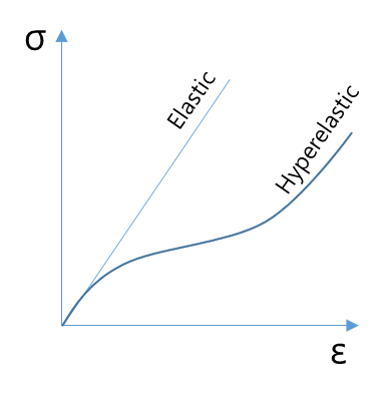
\includegraphics[scale=1]{Figures/Hyperelastic.png}
    \decoRule   
    \caption{ Difference between linear and non-linear material in stress–strain relationship}
    \label{fig:Electron}
\end{figure}
\end{list}
\end{itemize}
%------------------------------------------------------------------------------------------------
%-----------
\section{Finite Element Method (FEM) \parencite{ref4}}
In general, it is difficult to find an analytic solution that satisfies the variational
equation in the previous section. Instead, the FEM divides the entire domain into a
set of simple sub-domains or finite elements. The finite elements are connected with
adjacent elements by sharing their nodes. Then within each finite element, the
solution is approximated in a simple polynomial form.
\vspace{0.38cm}
\newline
FEMs for structural analysis require knowledge of the behavior of each element
in the structure. In this section, a structural analysis based on the finite element
approach is introduced using three-dimensional solid elements. Finite element for-
mulations for other structural elements, such as bars, beams, and plates, etc . Apart from the moreintricate algebra that is required for more complex elements, the basic approach for
deriving element equations is identical to the process illustrated in this section.
Once each element is described, the governing equations of the entire structure may
then be derived.

%------------------------------------------------------------------------------------------------
\section{Finite Element Approximation \parencite{ref4}}
Differential equations and variational equations, introduced in (\ref{theory}) page \pageref{theory},
are difficult to solve, except for a handful of simple cases. When the geometry is
complicated, it is not trivial to solve for u(x) analytically. Since the solution that
satisfies the differential equation and boundary conditions can have a complicated
expression, an infinite series solution may need to be employed. In the FEM, instead
of solving the variational equation analytically, an approximate solution is sought.
The approximate solution u(x) is expressed as a sum of a number of functions that
are called trial functions:
\begin{equation}
\label{eqn:1}
u(x) = \sum\limits_{i = 1}^n {{c_i}} {\phi _i}(x){\rm{ }}
\end{equation}
where $n$ is the number of terms used, $\phi_i(x)$ are known trial functions, and $c_i$ are
coefficients to be determined by minimizing error between the true and the approxi-
mate solution. Since the approximate solution is a linear combination of the trial
functions, the accuracy of approximation depends on them.
\vspace{0.38cm}
\newline
The trial functions and coefficients are chosen such that $u(x)$ must satisfy the
essential boundary conditions of the problem; that is, $u(x)$ must belong to the
space of kinematically admissible displacements, $\mathbb{Z}$. Therefore, if the solution to
the variational equation is approximated by a series of functions in the entire domain
of the problem, it is difficult to obtain the trial functions that satisfy the essential
boundary conditions. An important idea of the FEM is to divide the entire domain
into a set of simple sub-domains or finite elements and then to apply the approximation 
in Eq. (\ref{eqn:1}) on the element level. Then, it is unnecessary to build the trial
functions that satisfy the essential boundary conditions. Instead, only those elements
that include the essential boundary conditions need to have a special treatment.
The finite elements are connected with adjacent elements by sharing their nodes.
Then within each finite element, the solution is approximated using a simple
polynomial form. For example, let us assume that the domain is one-dimensional
and the exact solution is given as a dashed curve in Fig. \ref{fig:Piecewise}. When the entire domain is divided into sub-domains (finite elements), it is possible to approximate the
solution using piecewise continuous linear polynomials as shown in Fig. \ref{fig:Piecewise}.
Within each element, the approximate solution is linear. Two adjacent elements
have the same solution value at the shared node. As can be seen in the figure, when
more numbers of elements are used, the approximate piecewise linear solution will
converge to the exact solution. In addition, the approximation can be more accurate
if higher-order polynomials are used in each element.\\

\begin{figure}[h!]
    \centering
    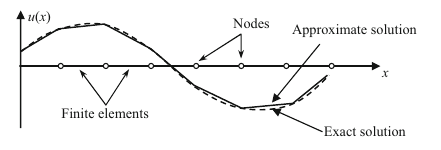
\includegraphics[scale=0.8]{Figures/Chapter2/Piecewise linear approximation.png}
    \decoRule   
    \caption{Piecewise linear approximation of the solution for one-dimensional problem}
    \label{fig:Piecewise}
\end{figure}

%--------------------------------------------------------------
\section{Numerical Integration \parencite{Advance}, \parencite{ref4}}

The integration of the components of the element stiffness matrix, the element mass matrix and
the consistent element load vector was analytically carried out in the previous chapters. In order to have in the development of complex finite elements an adequate tool for the integration of element quantities that are hardly integrable analytically, numerical integration is introduced
and examined for the truss example. By means of numerical integration, it is possible to integrate arbitrary functions in an approximate way. The essential advantages of numerical integration are summarized as follows:
\begin{itemize}
    \item Simplification of the integration
    \item Integration of analytically non-integrable functions
    \item Selective subintegration for elimination of defects from the element formulation
\end{itemize}
In opposition to these advantages there are actually limitations, too:
\begin{itemize}
    \item The generation of element matrices and vectors is numerically costly
     \item The element matrices and vectors are integrated inexactly 3

\end{itemize}

Within the framework of finite element methods, the so-called \textit{Gauss-Legendre Quadrature} has
established itself. The \textsc{Gauss-Legendre} Quadrature of a function $f(\xi 1)$ over the parameter
space $\xi_1 \in [−1, 1]$ is given by the sum
\begin{equation}
\label{eqn:2108}
     \int_{-1}^{1} f\left(\xi_{1}\right) d \xi_{1}=\sum_{i=1}^{n} \alpha^{i} f\left(\xi_{1}^{i}\right) 
\end{equation}
\begin{figure}[H]
    \centering
    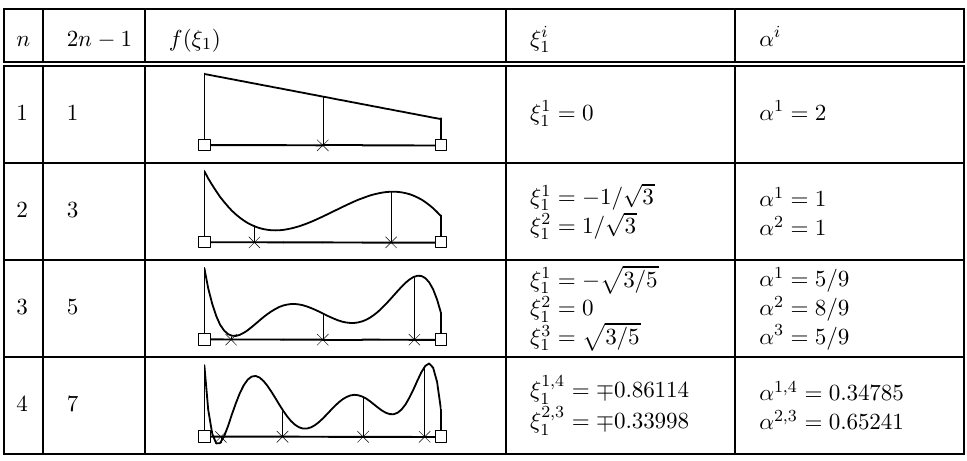
\includegraphics[scale=0.4]{Figures/Chapter2/quadrature.png}
    \caption{\textsc{Gauss} points $\xi_1^i$ and weight factors $\alpha^i$ of the \textsc{Gauss-Legendre} quadrature}
    \label{fig:222}
\end{figure}
In Eq. (\ref{eqn:2108}), $\alpha^i$ are the weight coefficients to the function values $f$ at the supports $\xi_1^i$ and n
is the number of integration points, or so-called \textit{Gauss points}. Polynomials of polynomial degree
\begin{equation}
    p\le 2n-1
\end{equation}
can be integrated exactly by \textsc{Gauss-Legendre} Quadrature, higher-order polynomials and other
functions can be integrated approximately. The linear, quadratic and cubic truss elements are
developed in this section by \textsc{Gauss-Legendre} integration with one and two supports. A summary of $\xi_1^i$ and $\alpha^i$ for $i = 1, 2, 3 $ is found in Figure \ref{fig:222}. For a representation of the fundamentals
of numerical integration, the way of obtaining of the weight factors $alpha^i$ and the \textsc{gauss} points $\xi_1^i$ , refer to the literature of numerical mathematics, e.g. \textsc{Deuflhard & Hohmann}

\textit{\underline{Example: Solve the equation:}}
\begin{equation*}
    x^3+x^2-5x=0
\end{equation*}
Code matlab and result for this problem :
\begin{lstlisting}
syms x;
F=x^3+x^2-5*x;
disp(int(F,[-1 1])); 
%% We take weight Gauss point from quadrature function
[Wgp,Qgp] = quadrature(5,'GAUSS',1); 
f=0;
%% Gauss Quadrature
for i=1 : size(Wgp,1)
    f=f+double(Wgp(i)*subs(F,x,Qgp(i)));
end
disp(f);
\end{lstlisting}

We have result for this example in Matlab : 
\begin{figure}[H]
    \centering
    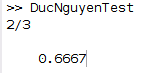
\includegraphics{Figures/Chapter2/resultQuadrature.png}
    \caption{Result for example Quadrature Problem}
    \label{fig:QDTP}
\end{figure}
%---------------------------------------------------------------
\section{Newton Raphson Method \parencite{NewtonRapsonBillboard} \parencite{ref4}}
The \textbf{Newton-Raphson method} (also known as Newton's method) is a way to quickly find a good approximation for the root of a real-valued function $f(x) = 0$ It uses the idea that a continuous and differentiable function can be approximated by a straight line tangent to it.
\subsection{How it Works ?}
Suppose you need to find the root of a continuous, differentiable function f(x)f(x), and you know the root you are looking for is near the point $x = x_0x=x 
0$. Then Newton's method tells us that a better approximation for the root is
\begin{equation}
 x_{1}=x_{0}-\frac{f\left(x_{0}\right)}{f^{\prime}\left(x_{0}\right)} 
\end{equation}
This process may be repeated as many times as necessary to get the desired accuracy. In general, for any $x$-value $x_n$ , the next value is given by
\begin{equation}
 x_{n+1}=x_{n}-\frac{f\left(x_{n}\right)}{f^{\prime}\left(x_{n}\right)} 
\end{equation}
\subsection{Geometric Representation}
Figure \ref{fig:nr1} is the picture to demonstrate what Newton's method actually does:
\begin{figure}[H]
    \centering
    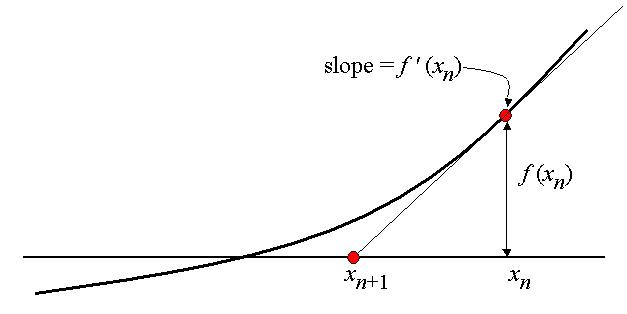
\includegraphics[scale=0.5]{Figures/Chapter2/newtonraphson1.png}
    \caption{Geometric Representation for \textbf{Newton-Raphson} method}
    \label{fig:nr1}
\end{figure}
We draw a tangent line to the graph of $f(x)$ at the point $x = x_n$. This line has slope $f'(x_n) $ and goes through the point $\big(x_n, f(x_n)\big)$
 Therefore it has the equation $y = f'(x_n)(x - x_n) + f(x_n)$. Now, we find the root of this tangent line by setting $y = 0$ and $x=x_{n+1}$ for our new approximation. Solving this equation gives us our new approximation, which is
 $
 x_{n+1}=x_{n}-\frac{f\left(x_{n}\right)}{f^{\prime}\left(x_{n}\right)} 
$
\subsection{Example With Matlab Code}
\label{Example2}
\vspace{0.38cm} \textit{Example: Find the root of the equation $x^2 - 4x - 7 = 0 $ near $x = 5$ to the nearest thousandth.}

We have our $x_0 = 5 $. In order to use Newton's method, we also need to know the derivative of ff. In this case, $f(x) = x^2 - 4x - 7$, and $f'(x) = 2x - 4$

Using Newton's method, we get the following sequence of approximations:
\begin{equation*}
    \begin{gathered}
{x_1} = 5 - \frac{{{5^2} - 4 \times 5 - 7}}{{2 \times 5 - 4}} = 5 - \left( {\frac{{ - 2}}{6}} \right) = \frac{{16}}{3} \approx 5.33333\\
{x_2} = \frac{{16}}{3} - \frac{{{{\left( {\frac{{16}}{3}} \right)}^2} - 4\left( {\frac{{16}}{3}} \right) - 7}}{{2\left( {\frac{{16}}{3}} \right) - 4}} = \frac{{16}}{3} - \frac{{\frac{1}{9}}}{{\frac{{20}}{3}}} = \frac{{16}}{3} - \frac{1}{{60}} = \frac{{319}}{{60}} \approx 5.31667\\
{x_3} = \frac{{319}}{{60}} - \frac{{{{\left( {\frac{{319}}{{60}}} \right)}^2} - 4\left( {\frac{{319}}{{60}}} \right) - 7}}{{2\left( {\frac{{319}}{{60}}} \right) - 4}} = \frac{{319}}{{60}} - \frac{{\frac{1}{{3600}}}}{{\frac{{398}}{{60}}}} \approx 5.31662.\\
{x_4} = 5.31662 - \frac{{{{(5.3362)}^2} - 4(5.3362) - 7}}{{2(5.3362) - 4}} = 5.31662
\end{gathered}
\end{equation*}

Code Matlab base on Newton-Raphson method:
\begin{lstlisting}
function [result,m]=NewtonRaphsonVsCount(x,f,range,n,x0)
%% input la bien so x, ham so f,range, so buoc lap n,x0 (neu co)
%output [result,m,]
%% giai thuat
df=diff(f,x,1);
ddf=diff(f,x,2);
newton= x-f/df;
%% Tim dieu kien bat dau bat fourier 
if exist('x0') == 0
    fourier=double(subs(f*ddf,x,range))
    for i =1:length(range)
        if fourier(i)>=0
            x0=range(i)
        end                             
    end
end
%% tim m de tinh sai so 
m=double(min(subs(abs(df), x, range)));
%% Bat dau giai thuat newton Raphson
X=[x0];
DeltaX=[0];
for i=1:n
    x_n=double(subs(newton,x,X(end)));
    X=[X;x_n];
    DeltaX=[DeltaX ; double(subs(abs(f)/m,x,x_n))];
end
n=[0:n]';
result=table(n,X,DeltaX);

\end{lstlisting}

We build solution for this example base on this function:
\begin{lstlisting}
syms x
range =[4 6];
f=x^2-4*x-7;
x0=5;
n=4;
[result]=NewtonRaphsonVsCount(x,f,range,n,x0);
disp(result)
\end{lstlisting}

\begin{figure}[H]
    \centering
    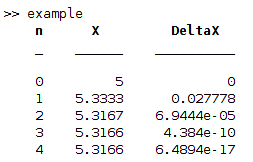
\includegraphics{Figures/Chapter2/resultNewton.png}
    \caption{Result for section \ref{Example2} in Matlab}
    \label{fig:Piecewise}
\end{figure}

\subsection{Limitations of Newton's Method}


Newton's method may not work if there are points of inflection, local maxima or minima around $x_0$  or the root.

For example, suppose you need to find the root of $27x^3 - 3x + 1 = 0$ which is near $x = 0$.
The correct answer is $-0.44157265\ldots$ However, Newton's method will give you the following:

\begin{equation*}
     x_{1}=\frac{1}{3}, x_{2}=\frac{1}{6}, x_{3}=1, x_{4}=0.679, x_{5}=0.463, x_{6}=0.3035, x_{7}=0.114, x_{8}=0.473, \ldots 
\end{equation*}

This is very clearly not helpful. That's because the graph of the function around $x = 0$ looks like in figure \ref{fig:limitNewton}.
\begin{figure}[H]
    \centering
    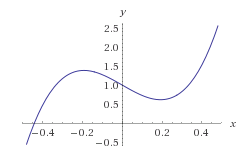
\includegraphics{Figures/Chapter2/limitNewton.png}
    \caption{Example the limit of \textsc{Newton-Raphson} Method }
    \label{fig:limitNewton}
\end{figure}
As you can see, this graph has a local maximum, a local minimum and a point of inflection around $x = 0$. To see why Newton's method isn't helpful here, imagine choosing a point at random between $x = -0.19$ and $x=0.19$ and drawing a tangent line to the function at that point. That tangent line will have a negative slope, and therefore will intersect the $y$-axis at a point that is farther away from the root. So this method doesn't always give the expected result.
\subsection{Significance of Newton-Raphson in Mechanical Solution }
Consider the following system of nonlinear equations:
\begin{equation}
\label{eqn:26}
    P(u)=f
\end{equation}
where $u = [u_1, u_2,\ldots,u^n]^T$ is a vector of unknowns, $f=4 [f_1, f_2,\ldots , f_n]^T$ is a vector of known quantities, and $P(u)= [P_1(u), P_2(u),\ldots, P_n(u)]^T$ is a vector of nonlinear
functions of $u$. In structural applications, $u$ is often the displacement vector, $f$ is the
applied force vector, and $P(u)$ is the internal force vector. Thus, Eq. (\ref{eqn:26}) is the
equilibrium between internal and applied forces. In the linear problems 
the internal force vector is a linear function of u such that $P(u)=K.u$ with $K$ being
a constant stiffness matrix. Then, solving a system of linear equations is equivalent
to calculating the inverse matrix of K and multiplying it with the vector,
$f$. 

Since P(u) is a nonlinear function of $u$, nonlinear analysis focuses on how to solve Eq. (\ref{eqn:26}) accurately and effectively. The solution methods applicable to general nonlinear functions are all iterative. Starting from an initial estimate, $u_0$, the increment, $\Delta u$, of the solution is obtained by solving a system of linear equations. Linearization is involved in this process. After obtaining the increment, the solution is iteratively updated until a specified convergence criterion is satisfied. Different methods are available according to the way to calculate the increment,
$\Delta u$; 

\textsc{Newton-Raphson} method is popular in numerical analysis to find the roots of nonlinear
equations. Basically, most numerical methods for solving a system of nonlinear
equations assume an initial estimate, u0, and find its increment, Δu, so that the
new estimate, $u_0 + \Delta u,$ is close to the solution to Eq. (\ref{eqn:26}). In order to find the increment, the nonlinear equations are locally approximated by linear ones. This process is repeated until the original nonlinear equations are satisfied. these will be discussed in section \ref{sec:nonlinear}.

%---------------------------------------------------------------
\section{Plane Finite Elements \parencite{ref6}}
The Finite Element Method (FEM) is used for finding approximate solutions of partial
differential equations. It is based on an expansion of the dependent variable(s), the
particle flux in our case, into a linear combination of polynomial trial functions defined
over subvolumes. The trial functions space must be chosen so as to ensure that improvement in the numerical approximation occurs with increase in the number I of subvolumes and/or
with the degree K of the polynomial trial functions. The trial functions are known a priori and the corresponding coefficients can be found using a weighted residual approach or a variational formulation. In this section, We have chosen to present the variational formulation, as it brings two important benefits:
\begin{enumerate}
    \item The intrinsic symmetry of the one-speed diffusion equation is always preserved by
the discretization process,
    \item The boundary conditions are introduced in a consistent way.
\end{enumerate} 

\begin{figure}[h!]
    \centering
    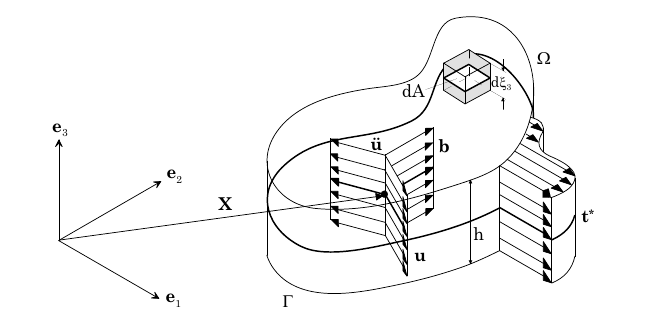
\includegraphics[scale=0.6]{Figures/Chapter2/planeElement.png}
    \decoRule   
    \caption{Representation of the three-dimensional continuum in plane elements}
    \label{fig:plane-element}
\end{figure}
\noindent
The FEM can be applied to various types and form of subvolumes or elements. In the following section first the basic equations of plane finite elements are derived from the
consideration of the three-dimensional continuum with the insertion of the fundamental assumptions of planar continua. Afterwards, plane elements are classified according to the element form and the order of the shape functions and the discretization of planar continua is explained in
details with the help of the four-node, linear, isoparametric Lagrange element. Furthermore,
retangular elements of higher approximation order and are discussed.
%--------
\subsection{Mechanical Problem}
\label{planeproblem}
In this section, we will discuss  two popular problems of the plane element: plane stress and plane strain
\begin{figure}[H]
    \centering
    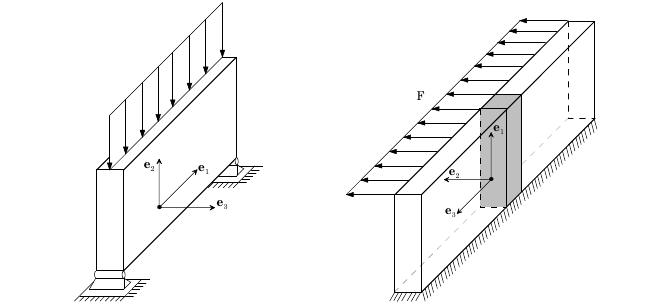
\includegraphics[scale=0.5]{Figures/Chapter2/110.png}
    \decoRule   
    \caption{ Examples for the application of plane stress and strain states}
    \label{fig:110}
\end{figure}
%-----plane strain stress
\vspace{0.38cm} \textbf{a) \textit{Plane Stress State}} \\
A representative plane element is examined, which lies in the plane spanned by the base vectors
$e_1$ and $e_2$ . In the case of a plane stress state it is assumed that the stress components $\sigma_{33}$ , $\sigma_{13}$ and $\sigma_{23}$ vanish

\begin{equation}
\begin{gathered}
  \sigma_{11}=\sigma_{22}=\sigma_{33}=0 \\
    \varepsilon_{13}=\varepsilon_{23}=0
\end{gathered}
\end{equation}
with the remaining stress components being constant in the direction of the base vector $e_3$ , see Fig. \ref{fig:111}
\begin{figure}[H]
    \centering
    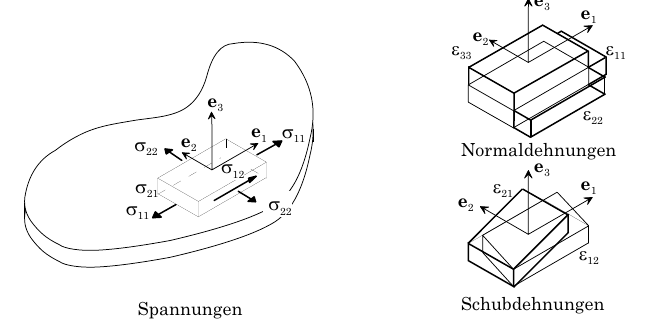
\includegraphics[scale=0.5]{Figures/Chapter2/111.png}
    \decoRule   
    \caption{Plane stress state}
    \label{fig:111}
\end{figure}
%-----plane strain stress
\vspace{0.38cm} \textbf{b) \textit{Plane Strain State}} \\
Again, a representative plane element is examined which lies in the plane spanned by the base
vectors $e_1$ and $e_2$ , see Fig.\ref{fig:112}. For the generation of the plane strain state it is assumed that the strain components $ \varepsilon_{33} , \varepsilon_{13}$ and $\varepsilon_{23} $vanish. the stress components $\sigma_{23} , \sigma_{13}$ become zero; the stress $\sigma_{33}$ , on the contrary, is different from zero.
\begin{equation}
\begin{gathered}
  \varepsilon_{11}=\varepsilon_{22}=\varepsilon_{33}=0 \\
    \sigma_{13}=\sigma_{23}=0
\end{gathered}
\end{equation}
\begin{figure}[H]
    \centering
    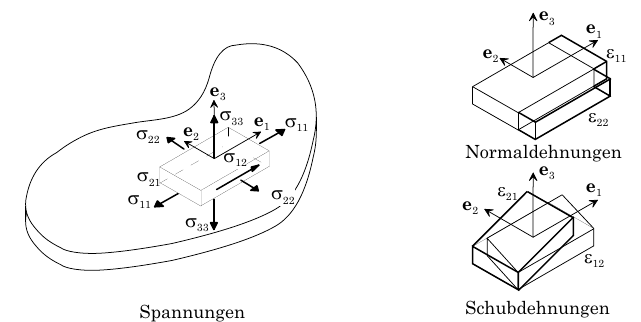
\includegraphics[scale=0.5]{Figures/Chapter2/112.png}
    \decoRule   
    \caption{  Plane strain state}
    \label{fig:112}
\end{figure}
%-------------------------------------------

%-----plane strain stress
\subsection{Geometry}
A planar structure, or a two-dimensional continuum, is generated by the degeneration of the
three-dimensional continuum onto a middle surface A and the thickness h. Due to this reason,
the properties of the three-dimensional continuum are represented by the properties of the
middle surface within the context of the modelling of a plane finite element (see Fig. \ref{fig:plane-element}).
Two-dimensional elements of structural mechanics are
\begin{itemize}
    \item Plane elements which are characterized by a small thickness $h$ relative to the dimensions of the middle surface and are characterized by the plane stress state ( see section \ref{planeproblem})
    
    \item Plane elements which describe an infinite dimension of the mechanical problem in $e _3$ - direction and are, thus, described by the plane strain state ( see section \ref{planeproblem}) 
\end{itemize}
\noindent
The thickness $h$ represents in the case of plane strain state the infinite thickness or the unit
thickness; therefore the thickness of finite elements of the plane strain state is often given the
value one. Within the context of this lecture the element thickness must be considered a parameter also for the plane strain state in order to guarantee a generalized description of elements of
the plane stress and strain state.
The geometrical description of such a two-dimensional element follows from the position vector
of a material point on the middle surface
\begin{equation}
    {\bf X}=[X_1 \quad X_2]^T
\end{equation}
and its motion when a load is applied.

%------------------------------------------------------------------------------------
%------------------------------------------------------------------------------------

\subsection{Kinetics}
The first fundamental assumption for the realization of the degeneration of the three- dimensional continuum to the two-dimensional continuum is the assumption of the stress and strain
state, where it is distinguished between the plane stress state (ES) and the plane strain state
(EV).
\begin{equation}
\label{eqn:3.2}
    \begin{gathered}
ES:{\sigma _{33}} = {\sigma _{23}} = {\sigma _{13}} = 0\\
EV:{\sigma _{33}} = \nu \left( {{\sigma _{11}} + {\sigma _{22}}} \right),{\sigma _{23}} = {\sigma _{13}} = 0
\end{gathered}
\end{equation}
When the plane stress state is assumed to hold the internal kinetics is uniquely described by
the components $\sigma_{11}$ , $\sigma_{22}$ and $\sigma_{12}$ (see Fig.1.11). In the case of plane strain state additionally
the normal stress component $\sigma_{33}$is present (see Fig. 1.12). For a complete and unique
characterization of the stress state this normal component of the stress tensor is actually not
necessary, as it can be computed directly from the stress components $\sigma_{11}$ and $\sigma_{22}$ according to
Eq. (1.74). For the formulation of the internal virtual work the component $\sigma_{33}$ is also of no
significance, for the conjugated strain component $\varepsilon_{33}$ is zero according to the assumptions of
the plane strain state. Therefore, it is enough, both for the plane stress state and for the plane
strain state, to define the stress vector
\begin{equation}
\label{eqn:3.3}
    \sigma=[\sigma_{11} \quad \sigma_{22} \quad \sigma_{33}]^T
\end{equation}

With three components for the formulation of the internal virtual work and, thus, also for the
generation of the discretized stiffness relation of plane finite elements. In accordance woth
the above-mentioned kinetic assumptions the volulme loads $b_3$ and the Neumann boundary
conditions $t^{*}_3$ vanish in the $e_3$-direction, wherefrom also the corresponding vectors are described
by two components each (see Fig. \ref{fig:110}).
\begin{equation}
\label{eqn:3.4}
 \boldsymbol{b}=\left[\begin{array}{ll}b_{1} & b_{2}\end{array}\right]^{T} \qquad \qquad \boldsymbol{t}^{\star}=\left[\begin{array}{ll}t_{1}^{\star} & t_{2}^{\star}\end{array}\right]^{T} 
\end{equation}

%----------------------------------------
\subsection{Kinematics}
The second fundamental assumption of plane finite elements concerns the displacement field:
all material points at the normal of the middle surface exhibit under deformation the same
displacements in the directions $e_1$ and $e_2$ .
\begin{equation}
\label{eqn:3.5}
 u_{1}=u_{1}\left(X_{1}, X_{2}\right) \qquad \qquad u_{2}=u_{2}\left(X_{1}, X_{2}\right) 
 \label{eqn:3.5}
\end{equation}

The displacement component $u_3$ is zero in the case of plane strain state. For the plane stress
state $u_ 3$ is different from zero. However, it follows from the assumptions for the volume and surface loads in Eq. (\ref{eqn:3.4}) that this displacement component has no contribution to the virtual
work of the external loads. Here, it is assumed without a proof 1 that also the portion of this component in the virtual wotk of the inertial forces vanishes during deformation. Thus, the
deformation of the degenerated two-dimensional continuum can be described uniquely by the displacement vector
\begin{equation}
 \boldsymbol{u}\left(X_{1}, X_{2}\right)=\boldsymbol{u}(\boldsymbol{X})=\left[\begin{array}{ll}u_{1}\left(X_{1}, X_{2}\right) & u_{2}\left(X_{1}, X_{2}\right)\end{array}\right]^{T} 
 \label{eqn:3.6}
\end{equation}
expressed, according to Eq. (\ref{eqn:3.5}), only in terms of the coordinates of the plane spanned by the
basis vectors e 1 and e 2 . From this follow directly the variation of the displacement vector and,
by twice differentiating Eq. (\ref{eqn:3.6}) with respect to time, the acceleration vector.
\begin{equation}
\label{eqn:3.7}
 \delta \boldsymbol{u}(\boldsymbol{X})=\left[\delta u_{1}\left(X_{1}, X_{2}\right) \quad \delta u_{2}\left(X_{1}, X_{2}\right)\right]^{T} \qquad \ddot{\boldsymbol{u}}(\boldsymbol{X})=\left[\begin{array}{ll}\ddot{u}_{1}\left(X_{1}, X_{2}\right) & \ddot{u}_{2}\left(X_{1}, X_{2}\right)\end{array}\right]^{T} 
\end{equation}

The complete description of the degenerated two-dimensional continuum requires furthermore the formulation of the Dirichlet boundary conditions
\begin{equation}
\label{eqn:3.8}
 \boldsymbol{u}(\boldsymbol{X}, t)=\boldsymbol{u}^{\star}(\boldsymbol{X}, t\qquad \qquad \forall \quad \boldsymbol{X} \in \Gamma_{u} 
\end{equation}
and the initial conditions of the displacement vector and the acceleration vector, where it should
be noted that only one of the two initial conditions has to be prescribed, as the second one results
from the evaluation of the equation of motion of the degenerated continuum at time $t = 0$
\begin{equation}
\label{eqn:3.9}
 \begin{aligned} \boldsymbol{u}(\boldsymbol{X}, t=0) &=\boldsymbol{u}^{\star}(\boldsymbol{X}) & \qquad \forall \quad \boldsymbol{X} \in \Omega \\ \ddot{\boldsymbol{u}}(\boldsymbol{X}, t=0) &=\ddot{\boldsymbol{u}}^{\star}(\boldsymbol{X}) & & \end{aligned} 
\end{equation}

It remains to describe the strain state of the degenerated continuum by the strain vector $\varepsilon$. In
accordance with the already discussed assumptions of plane stress or plane strain states this
vector can be obtained by the assembly of the strain components$\varepsilon_{ 11 }$, $\varepsilon_ {22}$ and $2\varepsilon_ {12}$ alone.
\begin{equation}
\label{eqn:3.10}
 \varepsilon=\left[\begin{array}{lll}\varepsilon_{11} & \varepsilon_{22} & 2 \varepsilon_{12}\end{array}\right]^{T} 
\end{equation}

The component $\varepsilon_{ 33 }$that is different from zero in the plane stress state is not needed for the unique characterization of the strain state, for this strain component can be combined linearly with the components $\varepsilon_{ 11}$ and $\varepsilon_{ 22}$ . In addition, the same argumentation
for the vanishing virtual work of the strain component $\varepsilon_{ 33}$ as in the definition of the stress vector
$\sigma$, applies here. The strain tensor can be computed in tensor notation
\begin{equation}
\label{eqn:3.11}
 \varepsilon=\nabla^{\mathrm{sym}} \boldsymbol{u} \qquad \qquad \varepsilon_{\alpha \beta}=\frac{1}{2}\left(u_{\alpha, \beta}+u_{\beta, \alpha}\right) 
\end{equation}
where it should be considered that the indices $\alpha$ and $\beta$ can take only the values one or two due to the degeneration ($\alpha$, $\beta$ = 1, 2). Besides, the strain vector can be obtained by application of the differential operator $D_\varepsilon$ to the displacement vector $u$.
\begin{equation}
\label{eqn:3.12}
 \varepsilon=\mathbf{D}_{\varepsilon} u \qquad \qquad
 \left[\begin{array}{c}\varepsilon_{11} \\ \varepsilon_{22} \\ 2 \varepsilon_{12}\end{array}\right]=\left[\begin{array}{cc}\frac{\partial}{\partial X_{1}} & 0 \\ 0 & \frac{\partial}{\partial X_{2}} \\ \frac{\partial}{\partial X_{2}} & \frac{\partial}{\partial X_{1}}\end{array}\right]\left[\begin{array}{l}u_{1} \\ u_{2}\end{array}\right] 
\end{equation}
Thus, it follows directly from the Eqs. (\ref{eqn:3.5}) that the components of the strain vector $\varepsilon_{\alpha \beta}$ are constant along the thickness of the degenerated continuum.

\begin{equation}
\label{eqn:3.13}
 \varepsilon=\varepsilon\left(X_{1}, X_{2}\right) 
\end{equation}
%----------------------------------------
\subsection{Finite Element Discretization}
The finite element discretization and analysis of plane continua consists of the partitioning of
the structure, or the domain under consideration, into finite elements and the approximation
of continuously distributed physical quantities (e.g. displacements) by discrete nodal degrees
of freedom and the assumption of their distribution over the element area. This assumption is
associated with the choice of shape functions, which depend on the variables $\varepsilon_1$ and $\varepsilon_2$ for the case of plane elements.

In contrast to the spatial truss frame, for which a constructively discrete structure was available
already before the mathematical discretization, now a two-dimensional continuum $\Omega$ must be
subdivided into finite subdomains $\Omega^e$ .
\begin{equation}
\label{eqn:3.28}
\begin{gathered}
    \Omega  = \bigcup\limits_{e = 1}^{NE} {{\Omega ^e}}\\
    with \quad {\Omega ^i} \cap {\Omega ^j} = \emptyset {\rm{ }} \quad for \quad i \ne 
\end{gathered}
\end{equation}

Inside these finite subdomains $\Omega^e$ , or finite elements $e$, the continuous field variables are approximated by means of shape functions and discrete nodal degrees of freedom. A basis for the
development of plane finite elements is the requirement that the principle of virtual work should
be fulfilled for every finite element $e$. 
\begin{equation}
\label{eqn:3.29}
 \delta W_{\mathrm{dyn}}^{e}+\delta W_{\mathrm{int}}^{e}=\delta W_{\mathrm{ext}}^{e} 
\end{equation}
The topological element structure, formed by the subdivision into subdomains $\Omega^e$ , is called finite element mesh and the process of its generation is meshing or mesh generation.

Accuracy of the finite element analysis increases with increasing the polynomial degree $p$, for which
reason the basic elements (3- or 4-node elements) are often substituted by elements of higher
polynomial degree. Furthermore, higher-order elements are essentially more suitable than the basic elements for discretizing domains $\Omega$ with curved boundaries, due to the possibility to
describe curved element boundaries. As is to be expected from the previous discussions, \textsc{Lagrange} elements with an internal node provide more accurate results than serendipity elements
without an internal node. The difference in the accuracy is, however, negligible and cannot level
out the shortcoming of the additionally needed internal degrees of freedom of the Lagrange
element (which are of importance particularly by the assembled system). As a disadvantage of
serendipity elements, it should be added that they are restricted to a polynomial degree $p < 4$

\subsection{Shape Functions of Plane Elements }
Within the framework of development of plane finite elements, shape functions of the varying
natural coordinates $\xi_1$ and $ \xi_2$ are used. These shape functions represent polynomials in the
two-dimensional space of the form


\begin{figure}
    \centering
    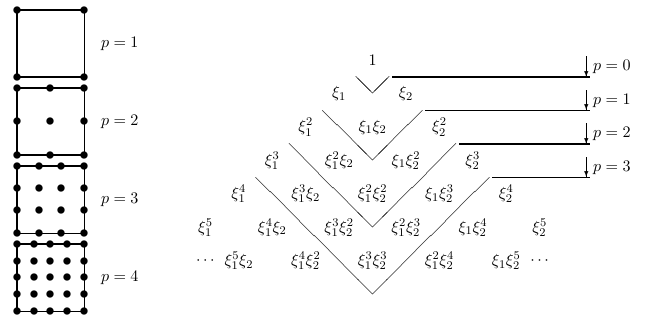
\includegraphics[scale=0.5]{Figures/Chapter2/LagrangePascal.png}
    \caption{Two-dimensional Lagrange ansatz polynomials of quadrangular elements in the
 \textsc{Pascal} triangle  }
    \label{fig:3.5}
\end{figure}


\begin{figure}
    \centering
    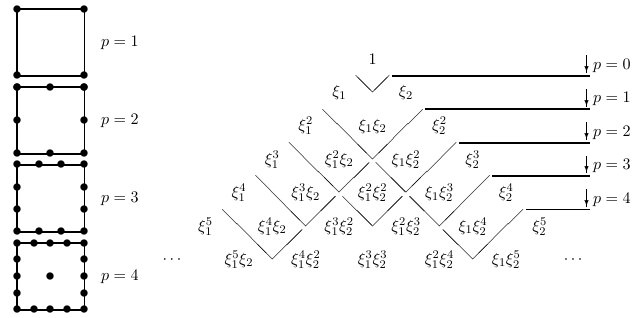
\includegraphics[scale=0.5]{Figures/Chapter2/polynomialsPascal.png}
    \caption{Two-dimensional Serendipity polynomials of quadrangular elements in the \textsc{Pascal}
triangle }
    \label{fig:3.6}
\end{figure}

where the terms of complete two-dimensional polynomials, which correspond to one polynomial
degree and are exempt from the coefficients $\alpha^{ij}$ , can be obtained from the Pascale’s triangle
in Fig. \ref{fig:3.5}. Within the context of development of plane finite elements, the shape functions $N^i (\xi_1 , \xi_2 )$, however, must be generated by multiplication of one-dimensional shape functions or on the basis of interpolation properties. In order to attain
already an idea of the qualitative differences of the finite elements developed in the following
chapters, these elements are characterized by means of the Pascale’s triangle, despite the
planned use of alternative methods for element development.

Complete polynomials of the degree p are derived by multiplication of two one-dimensional
polynomials, also of the degree $p$
\begin{equation}
\label{eqn:3.31}
 \boldsymbol{u}\left(\xi_{1}, \xi_{2}\right) \approx \tilde{\boldsymbol{u}}\left(\xi_{1}, \xi_{2}\right)=\left(\sum_{i=0}^{p} \alpha^{i}\left(\xi_{1}\right)^{i}\right)\left(\sum_{j=0}^{p} \alpha^{j}\left(\xi_{2}\right)^{j}\right) 
\end{equation}

Accordingly, the terms $(\xi_1)^i (\xi_2 )^j$ contained in the Pascale triangle are characterised by the
polynomial degree p of one of the two components paired with all potencies $\le p$ of the other
component. All used terms and thereby developed bilinear, biquadratic, bicubic and biquadratic
Lagrange quadrangular elements are summed up in figure \ref{fig:3.5}. 

\subsection{Serendipity bipolynomials}
Ansatz functions of the Serendipity type are generated with the help of the interpolation feature.
\begin{equation}
    {N^i}\left( {\xi _1^i,\xi _2^i} \right) = 1\qquad {N^i}\left( {\xi _1^j,\xi _2^j} \right) = 0\,\quad {\rm{with }}(i \ne j{\rm{ }})
\end{equation}
The corresponding terms in the Pascal triangle and the resulting finite Serendipity elements are
given in figure \ref{fig:3.6}. Compared to Lagrange ansatz functions, a lesser number of terms is being
used here, due to which a reduced accuracy can be expected compared to the corresponding
Lagrange elements. In order to guarantee at least complete polynomials, Serendipity ansatz
functions have to be furnished with an inner element node as well if the polynomial degree is
greater than $p = 4$, irrespective of the fact that their number is significantly smaller than it is
the case with \textsc{Lagrange} ansatz functions of the same polynomial degree
%---------------------------------------------------------------
\section{Bilinear Lagrange element (Q4) \parencite{LinearStructure}}
The development of plane finite elements is elaborated with the assistance of the relatively simply
generated four-noded bilinear Lagrange element and specified for the case of a rectangular
element.
\subsection{Shape Functions}
The shape function of element node one can be derived by multiplication of the one-dimensional
Lagrange polynomials $N_1^1 (\xi_1 )$ and $N_2^1 (\xi_2 )$ corresponding to this node, which are expressed
in the natural coordinate directions $\xi_1$ or $ \xi_2$ .
\begin{equation}
\label{eqn:3.33}
 N_{1}^{1}\left(\xi_{1}\right)=\frac{1}{2}\left(1-\xi_{1}\right) \quad N_{2}^{1}\left(\xi_{2}\right)=\frac{1}{2}\left(1-\xi_{2}\right) 
\end{equation}
Multiplication of $N_1^1(\xi_1)$ and $N_2^1(\xi_2)$ yields the shape function $N^1(\xi_ 1 , \xi_ 2 )$ for node one. The natural coordinates $\xi_ 1$ and $\xi_ 2$ are assembled in the vector $\xi_ = [\xi_ 1 \xi_ 2 ]$ T in order to show the dependencies.
\begin{equation}
\label{eqn:3.34}
    \label{eqn:334}
    \begin{split}
        {N^1}\left( {{\xi _1},{\xi _2}} \right) &= {N^1}(\xi ) = N_1^1\left( {{\xi _1}} \right)N_2^1\left( {{\xi _2}} \right) \\ &= \frac{1}{2}\left( {1 - {\xi _1}} \right)\frac{1}{2}\left( {1 - {\xi _2}} \right) = \frac{1}{4}\left( {1 - {\xi _1}} \right)\left( {1 - {\xi _2}} \right) \\ &= \frac{1}{4}\left( {1 - {\xi _1} - {\xi _2} + {\xi _1}{\xi _2}} \right)
    \end{split}
\end{equation}
As we can conclude from equation (\ref{eqn:334}), the shape function $N^1(\xi)$ contains constant, linear as
well as bilinear segments. In figure \ref{fig:3.6}, these segments correspond to the square in the Pascal
triangle characterised by $p = 1$. As a preliminary observation to the oncoming explanation of
approximating continuous variables, it may be noted that a two-dimensional polynomial of
plane elements is formed with the sum of all shape functions $N^i(\xi)$ that have the corresponding
weights. The shape functions of the element nodes two to four can be generated in an analogous way.
\begin{equation}
\label{eqn:3.35}
    \begin{gathered}
{N^1}(\xi ) = \frac{1}{4}\left( {1 - {\xi _1}} \right)\left( {1 - {\xi _2}} \right)\\
{N^2}(\xi ) = \frac{1}{4}\left( {1 + {\xi _1}} \right)\left( {1 - {\xi _2}} \right)\\
{N^3}(\xi ) = \frac{1}{4}\left( {1 + {\xi _1}} \right)\left( {1 + {\xi _2}} \right)\\
{N^4}(\xi ) = \frac{1}{4}\left( {1 - {\xi _1}} \right)\left( {1 + {\xi _2}} \right)
\end{gathered}
\end{equation}

Furthermore, in order to approximate the strains and to generate the Jacobi matrix, derivations
of shape functions with respect to the natural coordinates $\xi_ 1$ and $\xi_ 2$ are required. These can
be found as follows:
\[\arraycolsep=10pt\def\arraystretch{3.2}
\begin{equation}
\label{eqn:3.36}
\begin{array}{cccc}
{\dfrac{{\partial {N^1}({\boldsymbol{\xi }})}}{{\partial {\xi _1}}} = N_{;1}^1({\boldsymbol{\xi }}) =  - \dfrac{1}{4}\left( {1 - {\xi _2}} \right)}&{\dfrac{{\partial {N^1}({\boldsymbol{\xi }})}}{{\partial {\xi _2}}} = N_{;2}^1({\boldsymbol{\xi }}) =  - \dfrac{1}{4}\left( {1 - {\xi _1}} \right)}\\
{\dfrac{{\partial {N^2}({\boldsymbol{\xi }})}}{{\partial {\xi _1}}} = N_{;1}^2({\boldsymbol{\xi }}) = \dfrac{1}{4}\left( {1 - {\xi _2}} \right)}&{\dfrac{{\partial {N^2}({\boldsymbol{\xi }})}}{{\partial {\xi _2}}} = N_{;2}^2({\boldsymbol{\xi }}) =  - \dfrac{1}{4}\left( {1 + {\xi _1}} \right)}\\
{\dfrac{{\partial {N^3}({\boldsymbol{\xi }})}}{{\partial {\xi _1}}} = N_{;1}^3({\boldsymbol{\xi }}) = \dfrac{1}{4}\left( {1 + {\xi _2}} \right)}&{\dfrac{{\partial {N^3}({\boldsymbol{\xi }})}}{{\partial {\xi _2}}} = N_{;2}^3({\boldsymbol{\xi }}) = \dfrac{1}{4}\left( {1 + {\xi _1}} \right)}\\
{\dfrac{{\partial {N^4}({\boldsymbol{\xi }})}}{{\partial {\xi _1}}} = N_{;1}^4({\boldsymbol{\xi }}) =  - \dfrac{1}{4}\left( {1 + {\xi _2}} \right)}&{\dfrac{{\partial {N^4}({\boldsymbol{\xi }})}}{{\partial {\xi _2}}} = N_{i2}^4({\boldsymbol{\xi }}) = \dfrac{1}{4}\left( {1 - {\xi _1}} \right)}
\end{array}
\end{equation}
%---------------------------------------------------------
\subsection{Geometry}
The geometry of a four-noded Lagrange element in physical and natural space is shown in figure
\ref{fig:geometry}. An arbitrary material point within the quadrangular element is unequivocally identifiable
by its physical and natural coordinates.
\begin{equation}
 \boldsymbol{X}=\left[\begin{array}{lll}X_{1} & X_{2}\end{array}\right]^{T} \qquad \boldsymbol{\xi}=\left[\begin{array}{ll}\xi_{1} & \xi_{2}\end{array}\right]^{T} 
\end{equation}

Positions of the corner nodes are assembled in the element position vector.
\begin{equation}
    \begin{align}
{X^e} &= {\left[ {\begin{array}{*{20}{c}}
{X_1^{e1}}&{X_2^{e1}}&{X_1^{e2}}&{X_2^{e2}}&{X_1^{e3}}&{X_2^{e3}}&{X_1^{e4}}&{X_2^{e4}}
\end{array}} \right]^T}\\
&= {\left[ {\begin{array}{*{20}{c}}
{{X^e}^{1T}}&{{X^{e2}}^T}&{{X^{e3T}}}&{{X^{e4T}}}
\end{array}} \right]^T}
\end{align}
\end{equation}

Within the scope of isoparametric approximation of geometry and element variables, the continuous position vector $\boldsymbol{X}$ is described with the help of shape functions $N^i(\boldsymbol{\xi})$ in natural coordinates and with the help of discrete positions of element node $\boldsymbol{X}^e}$.

\begin{figure}
    \centering
    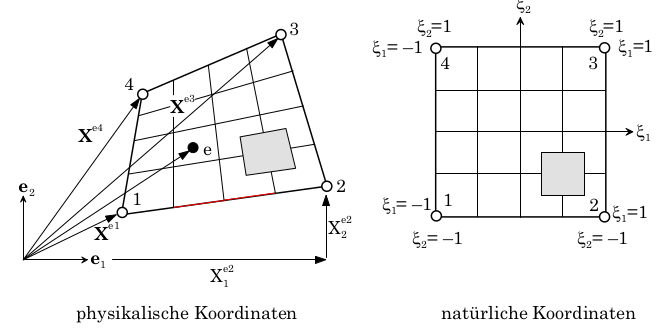
\includegraphics[scale=0.5]{Figure2/Chap2/Bilinear element.png}
    \caption{Bilinear element in physical and natural coordinates}
    \label{fig:geometry}
\end{figure}
\begin{equation}
\label{eqn:339}
 \boldsymbol{X}\left(\xi_{1}, \xi_{2}\right)=\boldsymbol{X}(\boldsymbol{\xi}) \approx \tilde{\boldsymbol{X}}(\boldsymbol{\xi})=\sum_{i=1}^{N \mathrm{~N}} \boldsymbol{X}^{e i} N^{i}(\boldsymbol{\xi})=\sum_{i=1}^{4} \boldsymbol{X}^{e i} N^{i}(\boldsymbol{\xi}) 
\end{equation}
where $NN$ generally stands for the number of element nodes. Alternatively, the continuous
position vector can be approximated by means of the shape function matrix $N(\boldsymbol{\xi})$ and with the
element position vector $\boldsymbol{X}^e$.
\vspace{0.1cm}
\begin{equation}
\small
\underbrace{\left[\begin{array}{c}
\tilde{X}_{1}(\xi) \\
\tilde{X}_{2}(\xi)
\end{array}\right]}_{\bar{X}(\xi)}=\underbrace{\left[\begin{array}{cccccccc}
N^{1}(\xi) & 0 & N^{2}(\xi) & 0 & N^{3}(\xi) & 0 & N^{4}(\xi) & 0 \\
0 & N^{1}(\xi) & 0 & N^{2}(\xi) & 0 & N^{3}(\xi) & 0 & N^{4}(\xi)
\end{array}\right]}_{N(\xi)} \underbrace{\left[\begin{array}{c}
X_{1}^{e 1} \\
X_{2}^{e 1} \\
X_{1}^{e 2} \\
X_{2}^{e 2} \\
X_{1}^{e 3} \\
X_{2}^{e 3} \\
X_{1}^{e 4} \\
X_{2}^{e 4}
\end{array}\right]}_{X^{e}}
\label{eqn:340}
\end{equation}

Equation (\ref{eqn:340}) describes the approximation of physical coordinates as function of natural
coordinates ($NN = 4$)
\begin{equation}
\label{eqn:341}
 \tilde{\boldsymbol{X}}(\boldsymbol{\xi})=\mathbf{N}(\boldsymbol{\xi}) \boldsymbol{X}^{e} \qquad \qquad \boldsymbol{X}^{e}=\left[\begin{array}{lllll}X_{1}^{e 1} & X_{2}^{e 1} & \cdots & X_{1}^{e N N} & X_{2}^{e N N}
\end{array}\right]^{T} 
\end{equation}
by means of shape function matrix $N(\boldsymbol{\xi})$, which is made up of diagonal matrices of shape
functions $N i (\boldsymbol{\xi})$ that correspond to element nodes $i$.
\begin{equation}
\label{eqn:3.42}
 \mathbf{N}^{i}(\boldsymbol{\xi})=\left[\begin{array}{cc}N^{i}(\boldsymbol{\xi}) & 0 \\ 0 & N^{i}(\boldsymbol{\xi})\end{array}\right] \qquad \qquad \mathbf{N}=\left[\begin{array}{lll}\mathbf{N}^{1} & \cdots & \mathbf{N}^{N N}\end{array}\right], NN=4 
\end{equation}

The mapping from natural to physical coordinates according to equations (\ref{eqn:339}) to (\ref{eqn:341}) can be generally described by the functional relation,
\begin{equation}
\label{eqn:3.43}
 \boldsymbol{X}=\boldsymbol{X}(\boldsymbol{\xi}) \qquad \qquad \qquad X_{\beta}=X_{\beta}(\boldsymbol{\xi}), \quad \beta=1,2 
\end{equation}
where the ’Tilda’ approximation designation is omitted. The inverse mapping describes the natural coordinates as function of the physical coordinates.
\begin{equation}
 \boldsymbol{\xi}=\boldsymbol{\xi}(\boldsymbol{X}) \qquad \qquad \qquad \xi_{\alpha}=\xi_{\alpha}(\boldsymbol{X}), \quad \alpha=1,2 
 \label{eqn:3.44}
\end{equation}
\subsection{Jacobi Transformation}
\begin{figure}
    \centering
    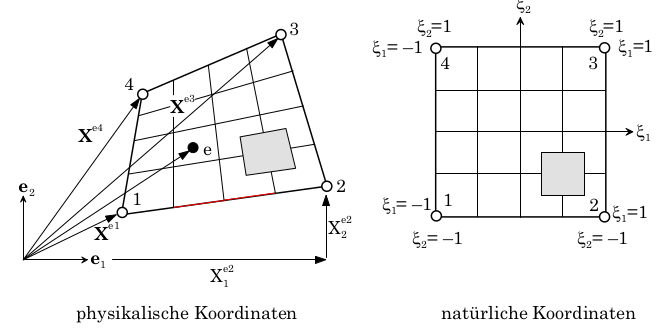
\includegraphics[scale=0.5]{Figure2/Chap2/Bilinear element.png}
    \caption{Jacobi transformation of a surface element $dA$ in natural coordinates}
    \label{fig:3.10}
\end{figure}
The calculation of the strain vector $\varepsilon$ according to equation (\ref{eqn:3.12}) requires that the displacement
components be derivated with respect to physical coordinates X. Since displacement components
as well as approximation of the position vector within the scope of the isoparametric element
concept are expressed as functions of natural coordinates, the necessary derivations with respect
to physical coordinates must be obtained indirectly over the partial derivatives of equation
(\ref{eqn:3.44}). Applying the chain rule to equation (\ref{eqn:3.44}) results in the transformation relation between derivatives with respect to physical and natural coordinates, respectively.
\begin{equation}
\label{eqn:3.45}
 \frac{\partial}{\partial \xi_{\alpha}}=\frac{\partial}{\partial X_{1}} \frac{\partial X_{1}}{\partial \xi_{\alpha}}+\frac{\partial}{\partial X_{2}} \frac{\partial X_{2}}{\partial \xi_{\alpha}}=\frac{\partial}{\partial X_{\beta}} \frac{\partial X_{\beta}}{\partial \xi_{\alpha}} 
\end{equation}

This equation can alternatively be given in the matrix form with the help of the Jacobi matrix $\boldsymbol{J(\xi)}$.
\begin{equation}

 \left[\begin{array}{c}\frac{\partial}{\partial \xi_{1}} \\ \frac{\partial}{\partial \xi_{2}}\end{array}\right]=\left[\begin{array}{ll}\frac{\partial X_{1}}{\partial \xi_{1}} & \frac{\partial X_{2}}{\partial \xi_{1}} \\ \frac{\partial X_{1}}{\partial \xi_{2}} & \frac{\partial X_{2}}{\partial \xi_{2}}\end{array}\right]\left[\begin{array}{c}\frac{\partial}{\partial X_{1}} \\ \frac{\partial}{\partial X_{2}}\end{array}\right] \qquad  \qquad \frac{\partial}{\partial \xi}=\mathbf{J}(\xi) \frac{\partial}{\partial \boldsymbol{X}} 
 \label{eqn:3.46}
\end{equation}

The rule for derivating functions in natural coordinates with respect to physical coordinates is
obtainable by inversion of equation (\ref{eqn:3.46}) with ${\rm{|J(}}\xi {\rm{)|  >  0}}{\rm{.}}$.
\begin{equation}
\label{eqn:3.47}
 \frac{\partial}{\partial \boldsymbol{X}}=\mathbf{J}^{-1}(\boldsymbol{\xi}) \frac{\partial}{\partial \boldsymbol{\xi}} 
\end{equation}
The inverse Jacobi matrix $J_{−1}(\xi)$ needed for this can be obtained directly by inverting the
$2 x 2 $ Jacobi matrix $J(\xi)$
\begin{equation}
\label{eqn:3.48}
 \mathbf{J}^{-1}(\boldsymbol{\xi})=\frac{1}{|\mathbf{J}(\boldsymbol{\xi})|}\left[\begin{array}{cc}\frac{\partial X_{2}}{\partial \xi_{2}} & -\frac{\partial X_{2}}{\partial \xi_{1}} \\ -\frac{\partial X_{1}}{\partial \xi_{2}} & \frac{\partial X_{1}}{\partial \xi_{1}}\end{array}\right] 
\end{equation}
where the Jacobi determinant is given by the expression
\begin{equation}
\label{eqn:3.49}
 |\mathbf{J}|=\frac{\partial X_{1}}{\partial \xi_{1}} \frac{\partial X_{2}}{\partial \xi_{2}}-\frac{\partial X_{1}}{\partial \xi_{2}} \frac{\partial X_{2}}{\partial \xi_{1}} 
\end{equation}
and the derivatives of physical coordinates are obtainable with respect to natural coordinates
from the approximation of the position vector $X = [X_1 X_2 ]^T $according to equations (\ref{eqn:339}) or (\ref{eqn:341}).
\begin{equation}
\label{eqn:3.50}
 \frac{\partial X_{\beta}(\boldsymbol{\xi})}{\partial \xi_{\alpha}}=\sum_{i=1}^{N} X_{\beta}^{e i} N_{; \alpha}^{i}(\boldsymbol{\xi}) \qquad \qquad \frac{\partial \boldsymbol{X}(\boldsymbol{\xi})}{\partial \xi_{\alpha}}=\boldsymbol{X}_{; \alpha}(\boldsymbol{\xi})=\mathbf{N}_{; \alpha}(\boldsymbol{\xi}) \boldsymbol{X}^{e} 
\end{equation}

Formally, we can get the inverse of the Jacobi matrix by applying the chain rule to functional
relation \( X_{\beta}=X_{\beta}(\boldsymbol{\xi}) \) given in equation (\ref{eqn:3.43})
\begin{equation}
\label{eqn:3.51}
 \frac{\partial}{\partial X_{\beta}}=\frac{\partial}{\partial \xi_{1}} \frac{\partial \xi_{1}}{\partial X_{\beta}}+\frac{\partial}{\partial \xi_{2}} \frac{\partial \xi_{2}}{\partial X_{\beta}}=\frac{\partial}{\partial \xi_{\alpha}} \frac{\partial \xi_{\alpha}}{\partial X_{\beta}} 
\end{equation}

Definition of the Jacobi matrix:
\begin{equation}
\label{eqn:3.52}
 \left[\begin{array}{c}\frac{\partial}{\partial X_{1}} \\ \frac{\partial}{\partial X_{2}}\end{array}\right]=\left[\begin{array}{cc}\frac{\partial \xi_{1}}{\partial X_{1}} & \frac{\partial \xi_{2}}{\partial X_{1}} \\ \frac{\partial \xi_{1}}{\partial X_{2}} & \frac{\partial \xi_{2}}{\partial X_{2}}\end{array}\right]\left[\begin{array}{c}\frac{\partial}{\partial \xi_{1}} \\ \frac{\partial}{\partial \xi_{2}}\end{array}\right]
 \qquad \qquad \frac{\partial}{\partial \boldsymbol{X}}=\mathbf{J}^{-1}(\xi) \frac{\partial}{\partial \xi} 
\end{equation}

By means of coefficient comparison of the inverse Jacobi matrix according to equations (\ref{eqn:3.48})
and (\ref{eqn:3.52}), we can get the identities
\begin{equation}
\label{eqn:3.53}
 \begin{aligned} \frac{\partial \xi_{1}}{\partial X_{1}} &=\frac{1}{|\mathbf{J}(\boldsymbol{\xi})|} \frac{\partial X_{2}}{\partial \xi_{2}} & \frac{\partial \xi_{2}}{\partial X_{1}} &=-\frac{1}{|\mathbf{J}(\boldsymbol{\xi})|} \frac{\partial X_{2}}{\partial \xi_{1}} \\ \frac{\partial \xi_{1}}{\partial X_{2}} &=-\frac{1}{|\mathbf{J}(\boldsymbol{\xi})|} \frac{\partial X_{1}}{\partial \xi_{2}} & \frac{\partial \xi_{2}}{\partial X_{2}} &=\frac{1}{|\mathbf{J}(\boldsymbol{\xi})|} \frac{\partial X_{1}}{\partial \xi_{1}} \end{aligned} 
\end{equation}

A transformation relation of the surface element $dA$ can be generated from the first of these
identities in physical and natural coordinates.
\begin{equation}
\label{eqn:3.54}
 d A=d X_{1} d X_{2}=|\mathbf{J}(\boldsymbol{\xi})| d \xi_{1} d \xi_{2} 
\end{equation}
Alternatively, we can derive these transformation relations that are presented in figure 3.10 with
assistance of surface elements, in physical and natural coordinates. For that purpose, vectors
$dX_ 1 , dX_ 2 , d\xi_1 $ and $d\xi$ 2 spanning the surface elements are defined. The surface elements are
given with the help of these definitions by the magnitude of the vector product of vectors $dX_ 1$
and $dX_ 2$ that is $d\xi_1$ and $d\xi_2$ .
\begin{equation}
\label{eqn:3.55}
 \begin{aligned} d A &=\left|d \boldsymbol{X}_{1} \times d \boldsymbol{X}_{2}\right| =\sin \alpha\left|d \boldsymbol{X}_{1}\right|\left|d \boldsymbol{X}_{2}\right| \\
  d A_{\xi} &=\left|d \xi_{1} \times d \boldsymbol{\xi}_{2}\right| =\sin \frac{\pi}{2}\left|d \boldsymbol{\xi}_{1}\right|\left|d \boldsymbol{\xi}_{2}\right| =d \xi_{1} d \xi_{2} \end{aligned} 
  \label{eqn:3.55} 
\end{equation}

Next, vectors $dX_\beta$ are tied with vectors $d\xi_\alpha$  with the help of equation (\ref{eqn:3.45}).
\begin{equation}
\label{eqn:3.56}
 d \boldsymbol{X}_{\beta}=\frac{\partial X_{\beta}}{\partial \xi_{\alpha}} d \boldsymbol{\xi}_{\alpha}=\frac{\partial X_{\beta}}{\partial \xi_{1}} d \boldsymbol{\xi}_{1}+\frac{\partial X_{\beta}}{\partial \xi_{1}} d \boldsymbol{\xi}_{1} 
 \label{eqn:3.56} 
\end{equation}

The square of surface element $dA$ comes as result of a vector scalar product of $d_1 x dX_2$ (see
equation (\ref{eqn:3.55})), where equation (\ref{eqn:3.56}) can be introduced instead of $dX_\beta$ .

\begin{equation}
\label{eqn:3.57}
 \begin{aligned} d A^{2}=&\left(d \boldsymbol{X}_{1} \times d \boldsymbol{X}_{2}\right) \cdot\left(d \boldsymbol{X}_{1} \times d \boldsymbol{X}_{2}\right)=\left(d \boldsymbol{X}_{1} \times d \boldsymbol{X}_{2}\right)^{2} \\=&\left[\left(\frac{\partial X_{1}}{\partial \xi_{1}} d \boldsymbol{\xi}_{1}+\frac{\partial X_{1}}{\partial \xi_{2}} d \boldsymbol{\xi}_{2}\right) \times\left(\frac{\partial X_{2}}{\partial \xi_{1}} d \boldsymbol{\xi}_{1}+\frac{\partial X_{2}}{\partial \xi_{2}} d \boldsymbol{\xi}_{2}\right)\right]^{2} \\=&[\frac{\partial X_{1}}{\partial \xi_{1}} \frac{\partial X_{2}}{\partial \xi_{1}} \underbrace{d \boldsymbol{\xi}_{1} \times d \boldsymbol{\xi}_{1}}_{\mathbf{0}}+\frac{\partial X_{1}}{\partial \xi_{1}} \frac{\partial X_{2}}{\partial \xi_{2}} d \boldsymbol{\xi}_{1} \times d \boldsymbol{\xi}_{2}\\ &+\frac{\partial X_{1}}{\partial \xi_{2}} \frac{\partial X_{2}}{\partial \xi_{1}} \underbrace{d \boldsymbol{\xi}_{2} \times d \boldsymbol{\xi}_{1}}_{-d \boldsymbol{\xi}_{1} \times d \boldsymbol{\xi}_{2}}+\frac{\partial X_{1}}{\partial \xi_{2}} \frac{\partial X_{2}}{\partial \xi_{2}} \underbrace{d \boldsymbol{\xi}_{2} \times d \boldsymbol{\xi}_{2}}_{\mathbf{0}}]^{2} \\=& \underbrace{\left[\frac{\partial X_{1}}{\partial \xi_{1}} \frac{\partial X_{2}}{\partial \xi_{2}}-\frac{\partial X_{1}}{\partial \xi_{2}} \frac{\partial X_{2}}{\partial \xi_{1}}\right]^{2}}_{|\mathbf{J}|^{2}} \underbrace{\left[d \boldsymbol{\xi}_{1} \times d \boldsymbol{\xi}_{2}\right]^{2}}_{d A_{\xi}^{2}}=|\mathbf{J}|^{2} d A_{\xi}^{2}=|\mathbf{J}|^{2} d \xi_{1}^{2} d \xi_{2}^{2} \end{aligned} 
 \label{eqn:3.57} 
\end{equation}

The Jacobi determinant here is identified by comparison to the Jacobi matrix determinant
according to equation (\ref{eqn:3.49}), and the surface element is obtained in natural coordinates by
means of comparison to equation (\ref{eqn:3.5}). The connection between the very surface elements
turns out to be trivial by forming the square root of equation (\ref{eqn:3.57}).
\begin{equation}
\label{eqn:3.58}
 d A=|\mathbf{J}(\boldsymbol{\xi})| d \xi_{1} d \xi_{2} 
\end{equation}

%-----------------------------------------
\subsection{Approximation of Element Quantities}
\begin{figure}[H]
    \centering
    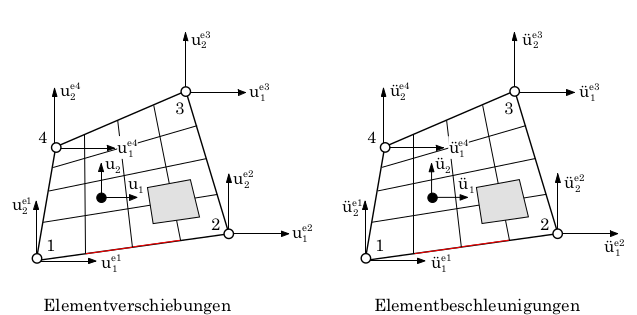
\includegraphics[scale=0.5]{Figure2/Chap2/4nodefredome.png}
    \caption{Degrees of freedom of a four-noded plane Lagrange element}
    \label{fig:3.11}
\end{figure}

Within the scope of the isoparametric element concept we can approximate the continuous
displacements, variation and second time derivative of displacements for $NN = 4$, analogous
with the approximation of the position vector in equation (\ref{eqn:341}) (see figure \ref{fig:3.11}).

\begin{equation}
 \begin{aligned} 
 \boldsymbol{u}(\boldsymbol{\xi}) & \approx \tilde{\boldsymbol{u}}(\boldsymbol{\xi})=\mathbf{N}(\boldsymbol{\xi}) \boldsymbol{u}^{e} & \boldsymbol{u}^{e} &=\left[\begin{array}
 {lllll}u_{1}^{e 1} & u_{2}^{e 1} & \cdots & u_{1}^{e N \mathrm{~N}} & u_{2}^{e N \mathbb{N}}
 \end{array}\right]^{T} \\ 
 \delta \boldsymbol{u}(\boldsymbol{\xi}) & \approx \delta \tilde{\boldsymbol{u}}(\boldsymbol{\xi})=\mathbf{N}(\boldsymbol{\xi}) \delta \boldsymbol{u}^{e} & \delta \boldsymbol{u}^{e} &= \left[
 \begin{array}{lllll}
     \delta u_{1}^{e 1}& \delta u_{2}^{e 1} &\cdots &\delta u_{1}^{e NN} &\delta u_{2}^{e N N}
 \end{array}
\right]^{T}   \\ 
 \ddot{\boldsymbol{u}}(\boldsymbol{\xi}) & \approx \tilde{\tilde{\boldsymbol{u}}}(\boldsymbol{\xi})=\mathbf{N}(\boldsymbol{\xi}) \ddot{\boldsymbol{u}}^{e} & \ddot{\boldsymbol{u}}^{e}
 &=\left[\begin{array}{lllll}\ddot{u}_{1}^{e 1} & \ddot{u}_{2}^{e 1} & \cdots & \ddot{u}_{1}^{e NN} & \ddot{u}_{2}^{e NN}\end{array}\right]^{T} 
 \end{aligned} 
 \label{eqn:3.59} 
\end{equation}

\subsection{Strain vector approximation}
To formulate the internal virtual work, the approximation of which is given with the help of
shape polynomials applied to displacements, and thereupon following integration of stiffness
terms, the strain vector components ought to be described in natural coordinates. This is ac-
complished by applying the derivation rule (\ref{eqn:3.51}) to the displacement strain relation in equation
\begin{equation}
\label{eqn:3.60} 
 \left[\begin{array}{c}\varepsilon_{11} \\ \varepsilon_{22} \\ 2 \varepsilon_{12}\end{array}\right]=\underbrace{\left[\begin{array}{ccc}\frac{\partial \xi_{1}}{\partial X_{1}} \frac{\partial}{\partial \xi_{1}}+\frac{\partial \xi_{2}}{\partial X_{1}} \frac{\partial}{\partial \xi_{2}} & 0 & \\ 0 & \frac{\partial \xi_{1}}{\partial X_{2}} \frac{\partial}{\partial \xi_{1}}+\frac{\partial \xi_{2}}{\partial X_{2}} \frac{\partial}{\partial \xi_{2}} \\ \frac{\partial \xi_{1}}{\partial X_{2}} \frac{\partial}{\partial \xi_{1}}+\frac{\partial \xi_{2}}{\partial X_{2}} \frac{\partial}{\partial \xi_{2}} & \frac{\partial \xi_{1}}{\partial X_{1}} \frac{\partial}{\partial \xi_{1}}+\frac{\partial \xi_{2}}{\partial X_{1}} \frac{\partial}{\partial \xi_{2}}\end{array}\right]}_{\mathbf{D}_{\varepsilon \xi}}\left[\begin{array}{c}u_{1} \\ u_{2}\end{array}\right], \quad \varepsilon=\mathbf{D}_{\varepsilon \xi} u 
\end{equation}

With the approximation of continuous displacements according to equation (\ref{eqn:3.59}), we get the
approximation of the strain vector from equation (\ref{eqn:3.60})
\begin{equation}
 \varepsilon(\boldsymbol{\xi}) \approx \tilde{\varepsilon}(\boldsymbol{\xi})=\mathbf{D}_{\varepsilon \xi}(\boldsymbol{\xi}) \tilde{\boldsymbol{u}}(\boldsymbol{\xi})=\mathbf{D}_{\varepsilon \xi}(\boldsymbol{\xi}) \mathbf{N}(\boldsymbol{\xi}) \boldsymbol{u}^{e}=\mathbf{B}(\boldsymbol{\xi}) \boldsymbol{u}^{e} \label{eqn:3.61} 
\end{equation}
by means of linear mapping of the element displacement vector and the differential operator
definition $\boldsymbol{B(\xi)}$.
\begin{equation}
\label{eqn:3.62}
 \tilde{\varepsilon}(\boldsymbol{\xi})=\mathbf{B}(\boldsymbol{\xi}) \boldsymbol{u}^{e} \qquad \qquad \mathbf{B}(\boldsymbol{\xi})=\mathbf{D}_{\varepsilon \xi}(\boldsymbol{\xi}) \mathbf{N}(\boldsymbol{\xi}) 
\end{equation}

The differential operator $B(\xi)$ is here given by applying $D \varepsilon\xi (\xi)$ to the matrix of shape functions
$N(\xi)$. If the operator $D _{\varepsilon\xi} (\xi)$ is not applied to the entire matrix of shape functions but only to
the submatrices $N i (\xi)$, we obtain the $B$-operator $B i (\xi)$ assigned to the element node i instead
of $B-operator B(\xi)$,
\begin{equation}
 \mathbf{B}_{i}(\boldsymbol{\xi})=\mathbf{D}_{\varepsilon \xi}(\boldsymbol{\xi}) \mathbf{N}^{i}(\boldsymbol{\xi}) \qquad  \qquad \mathbf{B}=\left[\begin{array}{lll}\mathbf{B}_{1} & \cdots & \mathbf{B}_{N \mathbf{N}}\end{array}\right], N N=4 
 \label{eqn:3.63} 
\end{equation}
with the differential operators $B_i(\xi)$ being matrix of the shape functions.
\begin{equation}
 \mathbf{B}_{i}(\boldsymbol{\xi})=\left[\begin{array}{ccc}\frac{\partial \xi_{1}}{\partial X_{1}} \frac{\partial}{\partial \xi_{1}}+\frac{\partial \xi_{2}}{\partial X_{1}} \frac{\partial}{\partial \xi_{2}} & 0 & \\ 0 & & \frac{\partial \xi_{1}}{\partial X_{2}} \frac{\partial}{\partial \xi_{1}}+\frac{\partial \xi_{2}}{\partial X_{2}} & \frac{\partial}{\partial \xi_{2}} \\ \frac{\partial \xi_{1}}{\partial X_{2}} \frac{\partial}{\partial \xi_{1}}+\frac{\partial \xi_{2}}{\partial X_{2}} \frac{\partial}{\partial \xi_{2}} & \frac{\partial \xi_{1}}{\partial X_{1}} \frac{\partial}{\partial \xi_{1}}+\frac{\partial \xi_{2}}{\partial X_{1}} & \frac{\partial}{\partial \xi_{2}}\end{array}\right]\left[\begin{array}{cc}N^{i}(\boldsymbol{\xi}) & 0 \\ 0 & N^{i}(\boldsymbol{\xi})\end{array}\right] 
 \label{eqn:3.64} 
\end{equation}

Finally, by applying the derivation rules we arrive at the portion of B-operator for element
node $i$.
\begin{equation}
 \mathbf{B}_{i}(\boldsymbol{\xi})=\left[\begin{array}{cc}\frac{\partial \xi_{1}}{\partial X_{1}} N_{; 1}^{i}(\boldsymbol{\xi})+\frac{\partial \xi_{2}}{\partial X_{1}} N_{; 2}^{i}(\boldsymbol{\xi}) & 0 \\ 0 & \frac{\partial \xi_{1}}{\partial X_{2}} N_{; 1}^{i}(\boldsymbol{\xi})+\frac{\partial \xi_{2}}{\partial X_{2}} N_{; 2}^{i}(\boldsymbol{\xi}) \\ \frac{\partial \xi_{1}}{\partial X_{2}} N_{; 1}^{i}(\boldsymbol{\xi})+\frac{\partial \xi_{2}}{\partial X_{2}} N_{; 2}^{i}(\boldsymbol{\xi}) & \frac{\partial \xi_{1}}{\partial X_{1}} N_{; 1}^{i}(\boldsymbol{\xi})+\frac{\partial \xi_{2}}{\partial X_{1}} N_{; 2}^{i}(\boldsymbol{\xi})\end{array}\right] 
 \label{eqn:3.65} 
\end{equation}


If the components of the inverse Jacobi matrix $\xi_{\alpha,\beta}$ according to equation (\ref{eqn:3.53}) are replaced by components of the Jacobi matrix $X_{\alpha,\beta}$ , it is possible to write down the $B$-operators $B_i (\xi)$ in the following way:
\begin{equation}
 \mathbf{B}_{i}(\boldsymbol{\xi})=\frac{1}{|\mathbf{J}(\boldsymbol{\xi})|}\left[\begin{array}{cc}\frac{\partial X_{2}}{\partial \xi_{2}} N_{; 1}^{i}(\boldsymbol{\xi})-\frac{\partial X_{2}}{\partial \xi_{1}} N_{; 2}^{i}(\boldsymbol{\xi}) & 0 \\ 0 & -\frac{\partial X_{1}}{\partial \xi_{2}} N_{; 1}^{i}(\boldsymbol{\xi})+\frac{\partial X_{1}}{\partial \xi_{1}} N_{; 2}^{i}(\boldsymbol{\xi}) \\ -\frac{\partial X_{1}}{\partial \xi_{2}} N_{; 1}^{i}(\boldsymbol{\xi})+\frac{\partial X_{1}}{\partial \xi_{1}} N_{; 2}^{i}(\boldsymbol{\xi}) & \frac{\partial X_{2}}{\partial \xi_{2}} N_{; 1}^{i}(\boldsymbol{\xi})-\frac{\partial X_{2}}{\partial \xi_{1}} N_{; 2}^{i}(\boldsymbol{\xi})\end{array}\right] 
 \label{eqn:3.66} 
\end{equation}

Derived in such a way, the B-operators contain matrix terms of the form $X _{\beta,\alpha} $ which again can be described as functions of shape function derivatives $N_{;a}^j(\xi)$ and of element node coordinates $X^{ij}_\beta$ according to equation (\ref{eqn:3.50}).
\begin{equation}
 \frac{\partial X_{\beta}}{\partial \xi_{\alpha}}=\frac{\partial}{\partial \xi_{\alpha}} \sum_{j=1}^{4} X_{\beta}^{e j} N^{j}(\boldsymbol{\xi})=\sum_{j=1}^{4} X_{\beta}^{e j} N_{; \alpha}^{j}(\boldsymbol{\xi}) 
 \label{eqn:3.67} 
\end{equation}
%--------------------------------------------------------------
\subsection{Appproximation of internal virtual work}

The internal virtual work is developed by substituting the stress vector by material law , by modifying the surface element $dA$ and by adjusting the integration
boundaries to natural coordinates $\xi_\alpha \in [{- 1}, 1]$.
\begin{equation}
 \delta W_{\mathrm{int}}^{e}=\int_{-1}^{1} \int_{-1}^{1} \delta \varepsilon(\boldsymbol{\xi}) \cdot \mathbf{C} \varepsilon(\boldsymbol{\xi})|\mathbf{J}(\boldsymbol{\xi})| h d \xi_{1} d \xi_{2} 
 \label{eqn:3.68} 
\end{equation}

Approximation of internal virtual work comes from substitution of the exact strain vector by
the approximated strain vector in equation (\ref{eqn:3.62})
\begin{equation}
 \delta \tilde{W}_{\mathrm{int}}^{e}=\int_{-1-1}^{1} \int_{-1}^{1} \delta \boldsymbol{u}^{e} \cdot \mathbf{B}^{T}(\boldsymbol{\xi}) \mathbf{C} \mathbf{B}(\boldsymbol{\xi}) \boldsymbol{u}^{e}|\mathbf{J}(\boldsymbol{\xi})| h d \xi_{1} d \xi_{2} 
 \label{eqn:3.69} 
\end{equation}

Due to the independence of the natural coordinates $\xi$ of both element displacement vectors $u^e$
and its variation $\epsilon u^e$ , both of these vectors can be exerted from the integral.

\begin{equation}
 \delta \tilde{W}_{\text {int }}^{e}=\delta \boldsymbol{u}^{e} \cdot \int_{-1}^{1} \int_{-1}^{1} \mathbf{B}^{T}(\boldsymbol{\xi}) \mathbf{C} \mathbf{B}(\boldsymbol{\xi})|\mathbf{J}(\boldsymbol{\xi})| h d \xi_{1} d \xi_{2} \boldsymbol{u}^{e}=\delta \boldsymbol{u}^{e} \cdot \mathbf{k}^{e} \boldsymbol{u}^{e} 
\label{eqn:3.70} 
\end{equation}

Here, we have defined the element stiffness matrix of a bilinear plane quadrangular element of
an arbitrary shape.
\begin{equation}
 \mathbf{k}^{e}=\int_{-1}^{1} \int_{-1}^{1} \mathbf{B}^{T}(\boldsymbol{\xi}) \mathbf{C} \mathbf{B}(\boldsymbol{\xi})|\mathbf{J}(\boldsymbol{\xi})| h d \xi_{1} d \xi_{2} 
\label{eqn:3.71} 
\end{equation}

The element thickness can be independent of the location in case of a plane stress state
$(h = h(\xi))$ ; in case of a plane strain state, the element thickness is constant. It is customary to add the integrand which is evaluated and weighed at the Gauss
points and formed with the help of the $B$-operator, the Jacobi determinant and the element
thickness, to the element stiffness matrix. The so called full integration or the $2 x 2$ integration
of a bilinear element accordingly requires four calculations of an integrand and its weighed
addition.
\begin{equation}
 \mathbf{k}^{e} \approx \sum_{i=1}^{2} \sum_{j=1}^{2} \alpha^{i} \alpha^{j} \mathbf{B}^{T}\left(\xi_{1}^{i}, \xi_{2}^{j}\right) \mathbf{C} \mathbf{B}\left(\xi_{1}^{i}, \xi_{2}^{j}\right)\left|\mathbf{J}\left(\xi_{1}^{i}, \xi_{2}^{j}\right)\right| h\left(\xi_{1}^{i}, \xi_{2}^{j}\right) 
 \label{eqn:3.72} 
\end{equation}

Gauss points $\xi_\alpha^i$ and weighting factors $\alpha^i$ of numeric integration can be found in figure \ref{fig:222}. Apart from the full integration, a subintegration of the bilinear element is also introduced with only
one Gauss point in the midpoint of the element. Merely in special cases of element geometry, it
is reasonable to determine the element stiffness by analytical derivation of the $B$-operator and analytical integration. 

\subsection{Approximation of dynamic virtual work}

Besides discretization of internal virtual work, transient mechanical problems also demand discretization of dynamic virtual work. If we, in the principle of virtual displacements, replace the surface element $dA$ and the integration boundaries 
\begin{equation}
 \delta W_{\mathrm{dyn}}^{e}=\int_{-1-1}^{1} \int_{1}^{1} \delta \boldsymbol{u}(\boldsymbol{\xi}) \cdot \ddot{\boldsymbol{u}}(\boldsymbol{\xi})|\mathbf{J}(\boldsymbol{\xi})| \rho h d \xi_{1} d \xi_{2} 
 \label{eqn:3.73} 
\end{equation}
and if we approximate the variation of displacements as well as continuous accelerations with
the assistance of shape functions according to equation (\ref{eqn:3.59}), we get the approximation of
virtual work of inertial forces.
\begin{equation}
 \delta \tilde{W}_{\mathrm{dyn}}^{e}=\delta \boldsymbol{u}^{e} \cdot \int_{-1-1}^{1} \int_{-1}^{1} \mathbf{N}^{T}(\boldsymbol{\xi}) \mathbf{N}(\boldsymbol{\xi})|\mathbf{J}(\boldsymbol{\xi})| \rho h d \xi_{1} d \xi_{2} \ddot{\boldsymbol{u}}^{e}=\delta \boldsymbol{u}^{e} \cdot \mathbf{m}^{e} \ddot{\boldsymbol{u}}^{e} 
 \label{eqn:3.74} 
\end{equation}

For purposes of defining the element mass matrix, we repeatedly took advantage of the fact
that the element vectors $\varepsilon u^e$ and $\ddot{o}^e$ are independent of natural coordinates.
\begin{equation}
 \mathbf{m}^{e}=\int_{-1}^{1} \int_{-1}^{1} \mathbf{N}^{T}(\boldsymbol{\xi}) \mathbf{N}(\boldsymbol{\xi})|\mathbf{J}(\boldsymbol{\xi})| \rho h d \xi_{1} d \xi_{2} 
\label{eqn:3.75} 
\end{equation}
\subsection{Approximation of virtual work of external loads}

The loads acting on a plane element can be divided into loads acting in the field and those acting at the boundaries of the field. Typical loads in the field are gravitational loads whereas actual structural loads are dominated by boundary loads such as pressure.

\vspace{0.38cm} \textbf{a) \textit{Volume loads}} \\

With the help of displacement variation approximation as in equation (\ref{eqn:3.59}), a consistent element load vector of volume loads $b(\xi)$ can be obtained based on external virtual work.
\begin{equation}
 \delta \tilde{W}_{\mathrm{ext}}^{\Omega e}=\delta \boldsymbol{u}^{e} \cdot \int_{-1}^{1} \int_{-1}^{1} \mathbf{N}^{T}(\boldsymbol{\xi}) \boldsymbol{b}(\boldsymbol{\xi})|\mathbf{J}(\boldsymbol{\xi})| \rho h d \xi_{1} d \xi_{2}=\delta \boldsymbol{u}^{e} \cdot \boldsymbol{r}_{p}^{e} 
\label{eqn:3.76} 
\end{equation}

Element vector of volume forces:

\begin{equation}
 \boldsymbol{r}_{p}^{e}=\int_{-1}^{1} \int_{-1}^{1} \mathbf{N}^{T}(\boldsymbol{\xi}) \boldsymbol{b}(\boldsymbol{\xi})|\mathbf{J}(\boldsymbol{\xi})| \rho h d \xi_{1} d \xi_{2} 
 \label{eqn:3.77} 
\end{equation}

Usually, $b$ is not given as dependent of natural coordinates $\xi$ but as function of physical
coordinates X. In such a case, the position of volume load has to be transformed to natural
coordinates $( b(X) \rightarrow b(\xi))$.

\vspace{0.38cm} \textbf{b) \textit{Boundary loads}} \\

The element load vector of element boundary loads $\boldsymbol{t*(\xi)}h$ is derived by observation of external virtual work . Here, the boundary $\Gamma$ σ can here be divided into four
boundaries $\Gamma_i$ i of the element.
\begin{equation}
 \delta W_{\mathrm{ext}}^{\Gamma e}=\int_{\Gamma_{\sigma}} \delta \boldsymbol{u} \cdot \boldsymbol{t}^{\star} h d \Gamma_{\sigma}=\sum_{i=1}^{4} \int_{\Gamma_{i}} \delta \boldsymbol{u} \cdot \boldsymbol{t}^{\star} h d \Gamma_{i}=\sum_{i=1}^{4} \delta W_{\mathrm{ext}}^{\Gamma_{i} e} 
 \label{eqn:3.78} 
\end{equation}

As an example, the proceeding for calculating the consistent equivalent loads is demonstrated
for element boundary three that connects nodes three and four. As shown in figure \ref{eqn:3.12}, the element edge is characterised by the natural coordinate $\xi_2 = 1$.

\begin{equation}
 \delta W_{\mathrm{ext}}^{\Gamma_{3 e}}=\int_{\Gamma_{3}} \delta \boldsymbol{u}\left(\xi_{1}, 1\right) \cdot \boldsymbol{t}^{\star}\left(\xi_{1}, 1\right) h d \Gamma_{3} 
 \label{eqn:3.79} 
\end{equation}

To integrate this integrand over element edge three, the line element $d\gamma_3$ must be transformed
into the natural coordinate $d\xi_1$ . The differential line element here is analysed in physical space. Projection of line element $d\gamma_3$ onto direction $e_1$ yields the differential physical line element $dX_ 1$ , projection onto direction $e_ 2$ yields $dX_2$ . Vice versa, the square of line element can be calculated with the Pythagoras theorem.
\begin{equation}
 d \Gamma_{3}^{2}=d X_{1}^{2}+d X_{2}^{2} 
 \label{eqn:3.80} 
\end{equation}
\begin{figure}
    \centering
    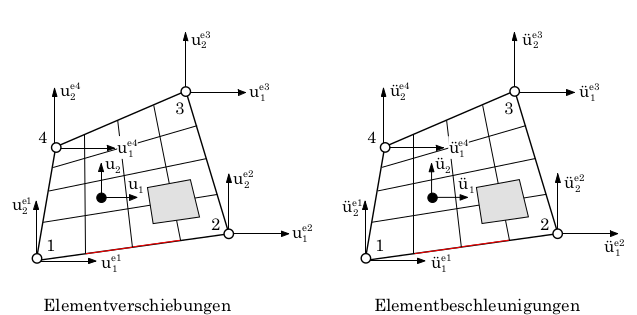
\includegraphics[scale=0.5]{Figure2/Chap2/4nodefredome.png}
    \caption{External loads of a four-noded Lagrange element}
    \label{fig:my_label}
\end{figure}

The total differentials $dX_\beta$ for $ \beta = 1, 2$ are found to be functions of total differentials in natural
coordinates and in Jacobi matrix components. It should be noted here that the differential $d\xi_2$
vanishes $(d\xi _2 = 0) $ at element edge three$ (\xi_ 2 = 1)$.
\begin{equation}
 d X_{\beta}=\frac{\partial X_{\beta}}{\partial \xi_{1}} d \xi_{1}+\frac{\partial X_{\beta}}{\partial \xi_{2}} d \xi_{2}=\frac{\partial X_{\beta}}{\partial \xi_{1}} d \xi_{1} 
\label{eqn:3.81}
\end{equation}

Inserting equation (\ref{eqn:3.81}) into equation (\ref{eqn:3.80}) yields the transformation relation of line element
$d\Gamma_3$ .

\begin{equation}
 d \Gamma_{3}^{2}=\left[\left(\frac{\partial X_{1}}{\partial \xi_{1}}\right)^{2}+\left(\frac{\partial X_{2}}{\partial \xi_{1}}\right)^{2}\right] d \xi_{1}^{2} 
 \label{eqn:3.82} 
\end{equation}

If we additionally introduce the Jacobi determinant$|J_3 (\xi_ 1 , 1)|$, which generally is a function of coordinate $\xi_1$ , we can write down the transformation relation (\ref{eqn:3.82}) in a familiar compact
form.
\begin{equation}
 d \Gamma_{3}=\left|\mathbf{J}_{3}\left(\xi_{1}, 1\right)\right| d \xi_{1} \quad\left|\mathbf{J}_{3}\left(\xi_{1}, 1\right)\right|=\left[\left(\frac{\partial X_{1}}{\partial \xi_{1}}\right)^{2}+\left(\frac{\partial X_{2}}{\partial \xi_{1}}\right)^{2}\right]^{\frac{1}{2}} 
 \label{eqn:3.83} 
\end{equation}

Formally, the same transformation relation is found for line element $d\Gamma_ 1$ , where the partial
derivatives in equation (3.81) must be evaluated for natural coordinate $\xi_ 2 = −1$ instead of
$\xi_ 2 = 1$. Analogous observations lead to transformation relation of line elements $d\Gamma_ 2$ and $d\Gamma_ 4$ .
Transformation of the line element $d\Gamma_ 4$ is given which is valid for both line elements.

\begin{equation}
 d \Gamma_{3}=\left|\mathbf{J}_{3}\left(\xi_{1}, 1\right)\right| d \xi_{1} \qquad \left|\mathbf{J}_{3}\left(\xi_{1}, 1\right)\right|=\left[\left(\frac{\partial X_{1}}{\partial \xi_{1}}\right)^{2}+\left(\frac{\partial X_{2}}{\partial \xi_{1}}\right)^{2}\right]^{\frac{1}{2}} 
 \label{eqn:3.84} 
\end{equation}
Back to element edge three and the boundary load of bilinear Lagrange elements. Next, the
position vector on the element edge according to equation (\ref{eqn:339}) is described with the help
of shape functions $N_ i (\xi_ 1 , 1), i = 1, 2, 3, 4 $, as a basis of transformation (\ref{eqn:3.83}). A reduction
of shape functions is not necessary here since the shape functions corresponding to element
nodes one and two vanish at the element edge three ($N_1 (\xi 1 , 1) = N_2 (\xi 1 , 1) = 0$, see equation
(\ref{eqn:3.35}) 
\begin{equation}
 \boldsymbol{X}\left(\xi_{1}, 1\right)=\sum_{i=1}^{4} \boldsymbol{X}^{e i} N^{i}\left(\xi_{1}, 1\right)=\sum_{i=3}^{4} \boldsymbol{X}^{e i} N^{i}\left(\xi_{1}, 1\right) 
 \label{eqn:3.85} 
\end{equation}

Derivative of the position vector with respect to natural coordinate $\xi_1$ is given by
\begin{equation}
 \frac{\partial \boldsymbol{X}\left(\xi_{1}, 1\right)}{\partial \xi_{1}}=\sum_{i=1}^{4} \boldsymbol{X}^{e i} N_{; 1}^{i}\left(\xi_{1}, 1\right)=\mathbf{N}_{; 1}\left(\xi_{1}, 1\right) \boldsymbol{X}^{e} 
 \label{eqn:3.86} 
\end{equation}
and the derivative with respect to $\xi_2$ is zero. Horizontal and vertical components $dX \beta , \beta = 1, 2$
of line element $ d\Gamma _3 $are found by calculation of total differentials according to equation (\ref{eqn:3.36}),
where derivatives of shape functions according to equation (\ref{eqn:3.81}) are directly used for $\xi_2 = 1$.
\begin{equation}
 d X_{\beta}=\frac{\partial X_{\beta}\left(\xi_{1}, 1\right)}{\partial \xi_{1}} d \xi_{1}=\left[X_{\beta}^{e 3} N_{; 1}^{3}\left(\xi_{1}, 1\right)+X_{\beta}^{e 4} N_{; 1}^{4}\left(\xi_{1}, 1\right)\right] d \xi_{1}=\left[X_{\beta}^{e 3} \frac{1}{2}-X_{\beta}^{e 4} \frac{1}{2}\right] d \xi_{1} 
 \label{eqn:3.87} 
\end{equation}

With equation (\ref{eqn:3.83}), the sought Jacobi determinant $|J_3 (\xi_ 1 , 1)|$ of a bilinear Lagrange element
finally follows, related to element edge three.
\begin{equation}
 \begin{aligned}\left|\mathbf{J}_{3}\left(\xi_{1}, 1\right)\right| &=\left[\left(X_{1}^{e 3} \frac{1}{2}-X_{1}^{e 4} \frac{1}{2}\right)^{2}+\left(X_{2}^{e 3} \frac{1}{2}-X_{2}^{e 4} \frac{1}{2}\right)^{2}\right]^{\frac{1}{2}} \\ &=\frac{1}{2}\left[\left(X_{1}^{e 3}-X_{1}^{e 4}\right)^{2}+\left(X_{2}^{e 3}-X_{2}^{e 4}\right)^{2}\right]^{\frac{1}{2}} \end{aligned}
 \label{eqn:3.88} 
\end{equation}

With this we can substitute the line element dΓ 3 in equation (\ref{eqn:3.79}) as well as the integration
boundaries by a differential of the natural coordinate $\xi_1 $ that is by interval boundaries of the
natural coordinate $\xi_1 \in [−1, 1]$.
\begin{equation}
 \delta W_{\mathrm{ext}}^{\Gamma_{3}}=\int_{-1}^{1} \delta \boldsymbol{u}\left(\xi_{1}, 1\right) \cdot \boldsymbol{t}^{\star}\left(\xi_{1}, 1\right) h\left|\mathbf{J}_{3}\left(\xi_{1}, 1\right)\right| d \xi_{1} 
 \label{eqn:3.89} 
\end{equation}

The approximation of displacement variation according to equation (\ref{eqn:3.59})
\begin{equation}
 \delta \tilde{W}_{\mathrm{ext}}^{\Gamma_{3}}=\delta \boldsymbol{u}^{e} \cdot \int_{-1}^{1} \mathbf{N}^{T}\left(\xi_{1}, 1\right) \boldsymbol{t}^{\star}\left(\xi_{1}, 1\right) h\left|\mathbf{J}_{3}\left(\xi_{1}, 1\right)\right| d \xi_{1}=\delta \boldsymbol{u}^{e} \cdot \boldsymbol{r}_{n 3}^{e} 
 \label{eqn:3.90} 
\end{equation}
finally yields the consistent equivalent load of the boundary load $r^e_{n3}$ .
\begin{equation}
 \boldsymbol{r}_{n 3}^{e}=\int_{-1}^{1} \mathbf{N}^{T}\left(\xi_{1}, 1\right) \boldsymbol{t}^{\star}\left(\xi_{1}, 1\right) h\left|\mathbf{J}_{3}\left(\xi_{1}, 1\right)\right| d \xi_{1} 
 \label{eqn:3.91} 
\end{equation}

The summation of all correspondingly calculated equivalent loads $r_{ni}$ for $i = 1, 2, 3, 4$ yields the
consistent equivalent loads of an element.
\begin{equation}
 \delta \tilde{W}_{\mathrm{ext}}^{\Gamma}=\sum_{i=1}^{4} \delta \tilde{W}_{\mathrm{ext}}^{\Gamma_{i}}=\sum_{i=1}^{4} \delta \boldsymbol{u}^{e} \cdot \boldsymbol{r}_{n i}^{e}=\delta \boldsymbol{u}^{e} \cdot \sum_{i=1}^{4} \boldsymbol{r}_{n i}^{e}=\delta \boldsymbol{u}^{e} \cdot \boldsymbol{r}_{n}^{e} 
 \label{eqn:3.92} 
\end{equation}

The integration of consistent equivalent loads according to equation (3.91) is performed mostly
numerically, too. As opposed to integration of $k _e , m_ e $or $r _{ep} $, one-dimensional numerical integration is necessary here. 
It may be noted here that virtual works of boundary loads of adjacent elements cancel each
other out. For this reason, it is sufficient to calculate the virtual works of boundary loads at free
boundaries that are not only element boundaries but also represent system boundaries.
%-------------------------------------------------------
\section{Biquadratic Serendipity Element (Q8) \parencite{LinearStructure}}
The considerable disadvantage of nine-noded biquadratic Lagrange elements compared to
a bilinear element is the increased number of degrees of freedom. Especially both degrees of
freedom of the middle node are increasing the linear equation system of the assembled system
which has to be solved by two equations per discrete Lagrange element. On the other hand, the
same middle node is not necessary for preservation of compatibility with the adjacent element.

This means that the number of degrees of freedom can especially be reduced at system level
by utilization of serendipity elements instead of Lagrange elements. Hence, the motivation for
generation of quadratic serendipity elements with no middle node is given.

In the sections that follow we will discuss shape functions, approximation of geometry and of
the displacement field. Since the development of the differential operator and of element matrices
and vectors has to be accomplished in analogy with the four-noded or nine-noded Lagrange
element, the presentation of this procedure is abandoned.
\begin{figure}[H]
    \centering
    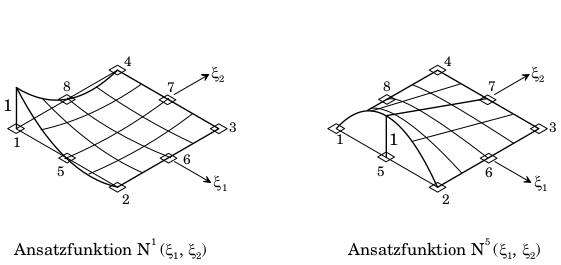
\includegraphics[scale=0.6]{Figure2/Chap2/shpaefunctionq8.png}
    \caption{Generation of biquadratic serendipity shape functions}
    \label{fig:my_label}
\end{figure}

\subsection{Shape Functions}
Contrary to a biquadratic \textsc{Lagrange} element, the shape functions of the eight-noded serendipity element cannot be generated from one-dimensional Lagrange interpolation functions. They
are constructed directly by means of the demands on shape function $N^i(\xi)$ to take on the value
one at node $i$ and the value zero at node $j \ne i$ . The generation of principally different shape functions of corner nodes and side middle nodes is shown in figure {\ref{fig:my_label}.
Here, as an example we have developed the shape functions of corner node one and side middle node eight.

The terms in $\xi_ 1$ and $\xi_ 2 $ appearing in shape functions $ N^ 1 , N^ 5$ and $N^ 8$ are designated by $p = 2$
in the Pascal triangle in figure \ref{fig:3.6}. The remaining shape functions of a quadratic serendipity element are written without deriving.
\begin{equation}
 \begin{aligned} N^{1}(\boldsymbol{\xi}) &=-\frac{1}{4}\left(1-\xi_{1}\right)\left(1-\xi_{2}\right)\left(1+\xi_{1}+\xi_{2}\right) & \qquad N^{5}(\boldsymbol{\xi}) &=\frac{1}{2}\left(1-\xi_{1}^{2}\right)\left(1-\xi_{2}\right) \\ N^{2}(\boldsymbol{\xi}) &=-\frac{1}{4}\left(1+\xi_{1}\right)\left(1-\xi_{2}\right)\left(1-\xi_{1}+\xi_{2}\right) & N^{6}(\boldsymbol{\xi}) &=\frac{1}{2}\left(1+\xi_{1}\right)\left(1-\xi_{2}^{2}\right) \\ N^{3}(\boldsymbol{\xi}) &=-\frac{1}{4}\left(1+\xi_{1}\right)\left(1+\xi_{2}\right)\left(1-\xi_{1}-\xi_{2}\right) & N^{7}(\boldsymbol{\xi}) &=\frac{1}{2}\left(1-\xi_{1}^{2}\right)\left(1+\xi_{2}\right) \\ N^{4}(\boldsymbol{\xi}) &=-\frac{1}{4}\left(1-\xi_{1}\right)\left(1+\xi_{2}\right)\left(1+\xi_{1}-\xi_{2}\right) & N^{8}(\boldsymbol{\xi}) &=\frac{1}{2}\left(1-\xi_{1}\right)\left(1-\xi_{2}^{2}\right) \end{aligned} 
\end{equation}
\subsection{Geometry}
The element coordinate vector X e has a dimension reduced by two as opposed to the vector $X^e$
of a Lagrange element, which corresponds to the coordinates of the middle node.
\begin{equation}
 \boldsymbol{X}^{e}=\left[\begin{array}{llllllll}\boldsymbol{X}^{e 1T} & \boldsymbol{X}^{e 2 T} & \boldsymbol{X}^{e 3 T} & \boldsymbol{X}^{e 4 T} & \boldsymbol{X}^{e 5 T} & \boldsymbol{X}^{\epsilon 6 T} & \boldsymbol{X}^{e 7 T} & \boldsymbol{X}^{e 8 T}\end{array}\right]^{T} 
 \label{eqn:3.151} 
\end{equation}

Geometry of a serendipity element is usually described as function of natural coordinates $\xi$
according to equation (\ref{eqn:3.42}) with the shape functions matrix
\begin{equation}
 \mathbf{N}^{i}(\boldsymbol{\xi})=\left[\begin{array}{cc}N^{i}(\boldsymbol{\xi}) & 0 \\ 0 & N^{i}(\boldsymbol{\xi})\end{array}\right] \quad \mathbf{N}(\boldsymbol{\xi})=\left[\begin{array}{ccccc}\mathbf{N}^{1} & \mathbf{N}^{2} & \cdots & \mathbf{N}^{7} & \mathbf{N}^{8}\end{array}\right] 
 \label{eqn:3.152} 
\end{equation}

%--------------------------------------------
\subsection{Jacobi Transformation}
The \textsc{Jacobi} matrix $J(\xi)$, that is the inverse Jacobi matrix necessary to generate the derivatives with respect to physical coordinates by means of derivatives with respect to natural coordinates,
can be computed in analogy according to equations (\ref{eqn:3.46}) that is (\ref{eqn:3.48}) or
(\ref{eqn:3.52}).
\begin{equation}
 \frac{\partial X_{\beta}(\boldsymbol{\xi})}{\partial \xi_{\alpha}}=\sum_{i=1}^{N N} X_{\beta}^{e i} N_{; \alpha}^{i}(\boldsymbol{\xi}) \qquad \qquad \frac{\partial \boldsymbol{X}(\boldsymbol{\xi})}{\partial \xi_{\alpha}}=\boldsymbol{X}_{; \alpha}(\boldsymbol{\xi})=\mathbf{N}_{; \alpha}(\boldsymbol{\xi}) \boldsymbol{X}^{e} 
 \label{eqn:3.143} 
\end{equation}

Transformation of a differential surface element $dA$ follows according to equation (\ref{eqn:3.58}) with the help of the Jacobi determinant.
%----------------------------------------
\subsection{Approximation of element quantities}

Element quantities, displacements, accelerations and variation of displacements are approxi-
mated in analogy with the Lagrange element.
\begin{equation}
 \begin{aligned} \boldsymbol{u}(\boldsymbol{\xi}) & \approx \tilde{\boldsymbol{u}}(\boldsymbol{\xi})=\mathbf{N}(\boldsymbol{\xi})  \boldsymbol{u}^{e} & \boldsymbol{u}^{e} &=\left[\begin{array}{lllll}u_{1}^{e 1} & u_{2}^{e 1} & \cdots & u_{1}^{e 8} & u_{2}^{e 8}\end{array}\right]^{T} \\ 
 \delta \boldsymbol{u}(\boldsymbol{\xi}) & \approx \delta \tilde{\boldsymbol{u}}(\boldsymbol{\xi})=\mathbf{N}(\boldsymbol{\xi}) \delta \boldsymbol{u}^{e} & \delta \boldsymbol{u}^{e}&=\left[ 
 \begin{array}{lllll}
 \delta u_{1}^{e 1} &\delta u_{2}^{e 1}& \cdots &\delta u_{1}^{e 8}& \delta u_{2}^{e 8}
 \end{array}
 \right]^{T} \\ 
 \ddot{\boldsymbol{u}}(\boldsymbol{\xi}) & \approx \tilde{\tilde{u}}(\boldsymbol{\xi})=\mathbf{N}(\boldsymbol{\xi}) \ddot{u}^{e} & \ddot{\boldsymbol{u}}^{e}&=\left[\begin{array}{lllll}\ddot{u}_{1}^{e 1} & \ddot{u}_{2}^{e 1} & \cdots & \ddot{u}_{1}^{e 8} & \ddot{u}_{2}^{e 8}\end{array}\right]^{T} \end{aligned} 
\end{equation}

The dimension of the element vector is by two smaller than that of an element with a middle
node. Element vectors $u _e$ , $\varepsilon u^e $and $\ddot{u}^ e$ are of dimension $16 × 1$ and the shape function matrix
$\boldsymbol{N}$ is of dimension $2 \times 16$.



% \section{Solution of Non-Linear Static Structural Equations}
% \label{sec:nonlinear}
\vspace{0.38cm}
\newline
With geometrical non-linearity, alterations regarding geometrically linear observation:
\begin{itemize}
    \item Consideration of non-linear terms of the strain tensor E (kinematics)
     \item Establishing the forces equilibrium or application of the impulse theorem in the deformed
configuration (kinetics)

\end{itemize}
We use: 

\begin{itemize}
    \item  (Total) Lagrange point of view which is also described as the material point of view
     \item Stress and strain quantities in the undeformed configuration (second Piola Kirchhoff
stress tensor and Green Lagrange strain tensor)

\end{itemize}



\subsection{Kinematics}
\begin{figure}[h]
    \centering
    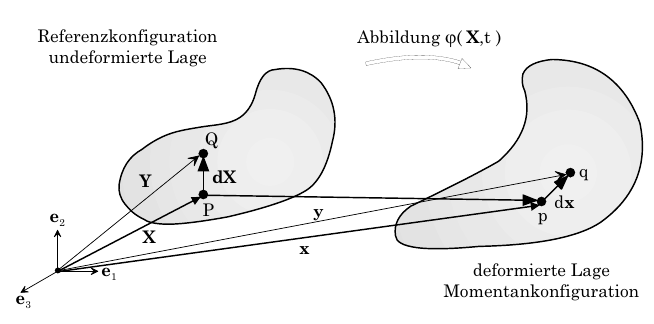
\includegraphics[scale=0.5]{Figures/Chapter2/anh3.png}
    \decoRule   
    \caption{ Current and reference configuration of a deformable material body}
    \label{fig:chap2anh3}
\end{figure}

\noindent
The fundamental of the geometrically non-linear formulation of structural mechanics is based on
the material deformation gradient F , which was already used within the scope of deriving the linear strain tensor  with the help of a non-linear deformation analysis of a material body, and
within the scope of subsequent linearization but not elaborated
because in linear observations it possesses no further significance. Non-linear observations are
a different story where the material deformation gradient defines the transformation from
reference to current configuration or from undeformed to deformed state and vice versa. These
transformations are referred to in technical literature as push forward and pull back. The
material deformation gradient is defined by a transformation of a line element dX of the
reference configuration to the current configuration dx (see figure \ref{fig:chap2anh3} ).

\begin{equation}
    dx = F \cdot dX; \quad F = \frac{{\partial x}}{{\partial X}} = \nabla x
\end{equation}
The Green Lagrange strain tensor E was also already derived and is given in equation (1.12) as function of the displacement gradient $\nabla u$ and its transpose ${\nabla ^T}u$. If we describe the
motion of the material point from the reference to the current configuration with help of the
displacement vector $\bf x = X + u$, the Green Lagrange strain tensor
\begin{equation}
    \label{5.7}
    E = \frac{1}{2}\left[ {{F^T} \cdot F - {\bf{1}}} \right] = {\nabla ^{{\rm{sym}}}}u + \frac{1}{2}{\nabla ^T}u \cdot \nabla u = \frac{1}{2}\left[ {{\nabla ^T}u + \nabla u + {\nabla ^T}u \cdot \nabla u} \right]
\end{equation}
can be represented as a function of the material deformation gradient.
\begin{equation}
 \boldsymbol{F}=\frac{\partial}{\partial \boldsymbol{X}}(\boldsymbol{X}+\boldsymbol{u})=\mathbf{1}+\nabla \boldsymbol{u} 
\end{equation}
According to this relation, the components of the term
\begin{equation}
 \nabla^{\operatorname{sym}} \boldsymbol{u}=\left[\begin{array}{ccc}u_{1,1} & \frac{1}{2}\left(u_{1,2}+u_{2,1}\right) & \frac{1}{2}\left(u_{1,3}+u_{3,1}\right) \\ \frac{1}{2}\left(u_{1,2}+u_{2,1}\right) & u_{2,2} & \frac{1}{2}\left(u_{2,3}+u_{3,2}\right) \\ \frac{1}{2}\left(u_{1,3}+u_{3,1}\right) & \frac{1}{2}\left(u_{2,3}+u_{3,2}\right) & u_{3,3}\end{array}\right] 
\end{equation}
of the linear part of the strain tensor E, given explicitly in equations (1.13) and (1.14), are
supplemented by the term $1/2 \nabla^T u$ · $\nabla u$, in the scope of geometrically non-linear theory, which can again be calculated with the displacement vector gradient according to eq. (1.7)
\begin{equation}
 \nabla \boldsymbol{u}=\left[\begin{array}{lll}u_{1,1} & u_{1,2} & u_{1,3} \\ u_{2,1} & u_{2,2} & u_{2,3} \\ u_{3,1} & u_{3,2} & u_{3,3}\end{array}\right] 
\end{equation}
by matrix multiplication.
\begin{equation}
 \frac{1}{2} \nabla^{T} \boldsymbol{u} \cdot \nabla \boldsymbol{u}=\frac{1}{2}\left[\begin{array}{lll}u_{k, 1}u_{k, 1} & u_{k, 1}u_{k, 2} & u_{k, 1} u_{k, 3} \\ u_{k, 2}u_{k, 1} & u_{k, 2}u_{k, 2} & u_{k, 2}u_{k, 3} \\ u_{k, 3}u_{k, 1} & u_{k, 3}u_{k, 2} & u_{k, 3}u_{k, 3}\end{array}\right] 
\end{equation}
It should be noted that the summation is performed over $k = 1, 2, 3$, respectively. The component presentation of the Green Lagrange strain tensor finally yields the following:
\begin{equation}
\label{5.12}
 E_{i j}=\frac{1}{2}\left(u_{i, j}+u_{j, i}+u_{k, i} u_{k, j}\right); \qquad \boldsymbol{E}=E_{i j} \boldsymbol{E}_{i} \otimes \boldsymbol{E}_{j} 
\end{equation}
In order to formulate the non-linear Finite Element methods, it remains to convert the calculation rule of the strain tensor, given in eq. (\ref{5.7}) or (\ref{5.12}), into the calculation rule of the strain
vector in a suitable way . The linear part of the strain tensor can be expressed as a vector by
application of the differential operator $D_\varepsilon$ to the displacement vector u, as described in eq.
(1.16). However, for the non-linear part of the strain tensor, no suitable operator presentation
can be found.
\begin{equation}
\label{5.13}
    {\bf{E}}({\bf{u}}) = \left[ {\begin{array}{*{20}{c}}
{{E_{11}}}\\
{{E_{22}}}\\
{{E_{33}}}\\
{2{E_{12}}}\\
{2{E_{23}}}\\
{2{E_{13}}}
\end{array}} \right] = \left[ {\begin{array}{*{20}{c}}
{{u_{1,1}}}\\
{{u_{2,2}}}\\
{{u_{3,3}}}\\
{{u_{1,2}} + {u_{2,1}}}\\
{{u_{2,3}} + {u_{3,2}}}\\
{{u_{1,3}} + {u_{3,1}}}
\end{array}} \right] + \left[ {\begin{array}{*{20}{l}}
{1/2\left( {{u_{1,1}}{u_{1,1}} + {u_{2,1}}{u_{2,1}} + {u_{3,1}}{u_{3,1}}} \right)}\\
{1/2\left( {{u_{1,2}}{u_{1,2}} + {u_{2,2}}{u_{2,2}} + {u_{3,2}}{u_{3,2}}} \right)}\\
{1/2\left( {{u_{1,3}}{u_{1,3}} + {u_{2,3}}{u_{2,3}} + {u_{3,3}}{u_{3,3}}} \right)}\\
{{u_{1,1}}{u_{1,2}} + {u_{2,1}}{u_{2,2}} + {u_{3,1}}{u_{3,2}}}\\
{{u_{1,2}}{u_{1,3}} + {u_{2,2}}{u_{2,3}} + {u_{3,2}}{u_{3,3}}}\\
{{u_{1,1}}{u_{1,3}} + {u_{2,1}}{u_{2,3}} + {u_{3,1}}{u_{3,3}}}
\end{array}} \right]{\rm{ }}
\end{equation}
According to eq (\ref{5.13}), the Green Lagrange strain tensor of geometrically non-linear
deformations is obtained by addition of the well-known linear part ${\bf D}_\varepsilon \bf u$ and the non-linear part $\bf E^\textnormal{nl}(u)$,
\begin{equation}
 \boldsymbol{E}(\boldsymbol{u})=\mathbf{D}_{\varepsilon} \boldsymbol{u}+\boldsymbol{E}^{n l}(\boldsymbol{u}) 
\end{equation}
where  ${\bf D}_\varepsilon \bf u$ and $\bf E^\textnormal{nl}(u)$ are defined as follows (summation over $k = 1, 2, 3$).

\begin{equation}
    {{\bf{D}}_\varepsilon }{\bf{u}} = \left[ {\begin{array}{*{20}{c}}
{{u_{1,1}}}\\
{{u_{2,2}}}\\
{{u_{3,3}}}\\
{{u_{1,2}} + {u_{2,1}}}\\
{{u_{2,3}} + {u_{3,2}}}\\
{{u_{1,3}} + {u_{3,1}}}
\end{array}} \right]\qquad {{\bf{E}}^{nl}}({\bf{u}}) = \left[ {\begin{array}{*{20}{l}}
{1/2}{{u_{k,1}}}{{u_{k,1}}}\\
{1/2}{{u_{k,2}}}{{u_{k,2}}}\\
{1/2}{{u_{k,3}}}{{u_{k,3}}}\\
{{u_{k,1}}}{{u_{k,2}}}{}\\
{{u_{k,2}}}{{u_{k,3}}}{}\\
{{u_{k,1}}}{{u_{k,3}}}{}
\end{array}} \right]
\end{equation}



 
%% Chapter 3

\chapter{ Finite element algorithms for contact problems \parencite{CONTACTBOOK} \parencite{ref4} } % Main chapter title

\label{Chapter4} % For referencing the chapter elsewhere, use \ref{Chapter1} 

%----------------------------------------------------------------------------------------

\section{Introduction}
Boundary value problems involving contact are of great importance in industrial applications
in mechanical and civil engineering. The range of application includes metal forming
processes, drilling problems, bearings, crash analysis of cars, car tires or cooling of electronic
devices. Other applications are related to biomechanics where human joints, implantats or
teeth are of consideration. Due to this variety contact problems are today combined either
with large elastic or inelastic deformations including time dependent responses. Thermal
coupling might have to be considered, see the cooling of electronic devices, the heat removal
within nuclear power plant vessels or thermal insulation of astronautic vehicles. Even
stability behaviour has to be linked to contact, like wrinkling arising in metal forming
problems.

Due to this technical importance a great number of researchers have investigated contact
problems. In the ancient egypt people needed to move large stone blocks to build the
pyramids and thus had to overcome the frictional force associated with it. Thus many known
researchers in the past have investigated frictional contact problems, amongst them were
Da Vinci, Amontons, Newton, Coulomb. Their investigations were based on the assumption
of rigid bodies. Starting with the classical analytical work of Hertz (1882) on the elastic
contact of two spheres the deformation of the bodies being in contact has been taken into
account. However only very few problems involving contact can be solved analytically. Thus
for most industrial applications numerical methods have to be applied when the contacting
bodies have complex geometries . Due to that the solution of contact problems with finite
element methods has a relatively long history, see Wilson, Parsons (1970) or Chan, Tuba
(1971) for early treatments.

In this overview article we will restrict ourselves mainly to finite element techniques for
the treatment of contact problems despite many other numerical schemes and analytical
approaches could be discussed as well. Furthermore we like to note that the description
of the mechanical behaviour of the bodies coming into contact will not be investigated in
detail, although this is of great importance. This article thus concentrates on the behaviour
in the contact interface. The associated formulation and discretization within the finite
element method will be considered as well as the development of algorithms.
\section{Contact Geometry}
This section summarizes relations which are necessary to formulate the geometrical contact
conditions. In detail the penetration and the relative slip in the contact area are discussed.
The first condition also includes the non–penetration condition which is used classically in
contact mechanics.

We assume that two bodies which undergo large deformations can come into contact.
Let $\mathcal{B}^\gamma$ , $ \gamma= 1, 2$ , denote the two bodies of interest and $\boldsymbol{\varphi}_{t}^{\gamma}: \mathcal{B}^{\gamma} \rightarrow \mathbb{R}^{3}$ the associated
deformation maps at time $t \in \mathbb{R}$. $\phi_t^{\gamma}$ maps points $\boldsymbol{X}^\gamma \in \mathcal{B}^\gamma$ of the reference configuration
onto points $x^\gamma = \phi ^\gamma_t(X^\gamma)$ of the current configuration.

%---------------------------------------------------
\section{Penetration}
As the first relevant function for the contact geometry we define a penetration function on
the current slave surface $\phi _t^1(\Gamma_c^1)$ by setting
\begin{equation}
 g_{N+}=\left\{\begin{array}{ll}\left\|\mathbf{x}^{1}-\hat{\mathbf{x}}_{t}^{2}\left(\bar{\xi}^{1}, \bar{\xi}^{2}\right)\right\| & \text { for }\left[\mathbf{x}^{1}-\hat{\mathbf{x}}_{t}^{2}\left(\bar{\xi}^{1}, \bar{\xi}^{2}\right)\right] \cdot \overline{\mathbf{n}}^{2}<0 \\ 0 & \text { otherwise }\end{array}\right. 
 \label{eqn:4.1} 
\end{equation}

Here $(\hat{\xi}^1,\hat{\xi}^2)$ is the minimizer of the distance function for a given slave point $x^1$
\begin{equation}
 \hat{d}^{1}\left(\xi^{1}, \xi^{2}\right)=\left\|\mathbf{x}^{1}-\hat{\mathbf{x}}_{t}^{2}\left(\xi^{1}, \xi^{2}\right)\right\| \longrightarrow \mathrm{MIN} 
 \label{eqn:4.2} 
\end{equation}

The values  $(\hat{\xi}^1,\hat{\xi}^2)$ are obtained by writing the necessary condition for the minimum of
the distance function (\ref{eqn:4.2})
\begin{equation}
 \frac{d}{d \xi^{\alpha}} \hat{d}^{1}\left(\xi^{1}, \xi^{2}\right)=\frac{\mathbf{x}^{1}-\hat{\mathbf{x}}_{t}^{2}\left(\xi^{1}, \xi^{2}\right)}{\left\|\mathbf{x}^{1}-\hat{\mathbf{x}}_{t}^{2}\left(\xi^{1}, \xi^{2}\right)\right\|} \cdot \hat{\mathbf{x}}_{t, \alpha}^{2}\left(\xi^{1}, \xi^{2}\right)=0
 \label{eqn:4.3} 
\end{equation}

The solution of (\ref{eqn:4.3}) requires the orthogonality of the first and second term. Since
$ \hat{\mathbf{x}}_{t, \alpha}^{2}\left(\xi^{1}, \xi^{2}\right) 
$  is the tangent vector $a^_\alpha$ the first term must denote the normal $n^2$ . Thus we
have the condition $-n^2 \cdot a^2_\alpha=0$ which means that the current master point $ \hat{\mathbf{x}}_{t}^{2}\left(\xi^{1}, \xi^{2}\right) 
$ is
the orthogonal projection of a given slave point $x^1$ onto the current master surface $\phi_t^2(\Gamma^2_c)$ .

Here and in the following we will denote by a bar over a quantity its evaluation at the
minimal distance point $\left(\overline{\xi}^{1}, \overline{\xi}^{2}\right)$ which means that these values denote the solution point of
(\ref{eqn:4.3}). Thus $\overline{\mathbf{n}}^{2}:=\left(\overline{\mathbf{a}}_{1}^{2} \times \overline{\mathbf{a}}_{2}^{2}\right) /\left\|\overline{\mathbf{a}}_{1}^{2} \times \overline{\mathbf{a}}_{2}^{2}\right\|$ is the outward unit normal on the current master
surface at the master point where $\overline{a}_\alpha^2$ are tangent vectors at $\hat{\mathbf{x}}_{t}^{2}\left(\overline{\xi^{1}}, \overline{\xi^{2}}\right)$.

The penetration function (\ref{eqn:4.1}) contains two informations:
\begin{enumerate}
    \item $g_{N+} $ serves as a local contact check, i.e. we set: $\text{contact} \Leftrightarrow	 g_{ N + }> 0$
    \item  $g_{N+} $ enters for $g_{N+} > 0$as a local kinematical variable the constitutive function for the contact pressure.
\end{enumerate}

By taking the time derivative of (\ref{eqn:4.2}) at the minimal distance point $\left(\overline{\xi}^{1}, \overline{\xi}^{2}\right)$ ) one obtains,
in the case of contact, the rate of penetration
\begin{equation}
 \dot{g}_{N+}=\left[\mathbf{v}_{t}^{1}-\hat{\mathbf{v}}_{t}^{2}\left(\bar{\xi}^{1}, \bar{\xi}^{2}\right)\right] \cdot \overline{\mathbf{n}}^{2} 
 \label{eqn:4.4} 
\end{equation}
for given spatial velocities $v_t^1 $ and $\hat{v}_t^2\left(\overline{\xi}^{1},\overline{\xi}^{2}\right)$  at the slave and master points.
%------------------------------------------------------------------------------
\section{Tangential Relative Velocity and Tangential Relative Slip}
The tangential relative slip between two bodies is related to the change of the solution point
$( \overline{\xi}^1 , \overline{\xi}^2)$ of the minimal distance problem. Thus we can compute the time derivative of $\xi^ \alpha$
from (\ref{eqn:4.3}). This yields the following result 
\begin{equation}
 \frac{d}{d t}\left\{\left[\mathbf{x}_{t}^{1}-\hat{\mathbf{x}}_{t}^{2}\left(\bar{\xi}^{1}, \bar{\xi}^{2}\right)\right] \cdot \overline{\mathbf{a}}_{\alpha}^{2}\right\}=\left[\mathbf{v}_{t}^{1}-\hat{\mathbf{v}}_{t}^{2}\left(\bar{\xi}^{1}, \bar{\xi}^{2}\right)-\overline{\mathbf{a}}_{\beta}^{2} \dot{\overline{\xi}}^{\beta} \right] \cdot \overline{\mathbf{a}}_{\alpha}^{2}+\left[\mathbf{x}_{t}^{1}-\hat{\mathbf{x}}_{t}^{2}\left(\bar{\xi}^{1}, \bar{\xi}^{2}\right)\right] \cdot \dot{\overline{\mathbf{a}}}_{\alpha}^{2}=0 
 \label{eqn:4.7} 
\end{equation}
with $\dot{\overline{{\mathbf{a}}}}_{\alpha}^{2}=\hat{\mathbf{v}}_{t, \alpha}^{2}\left(\bar{\xi}^{1}, \bar{\xi}^{2}\right)+\hat{\mathbf{x}}_{t, \alpha \beta}^{2}\left(\bar{\xi}^{1}, \overline{\xi}^{2}\right) \dot{\overline{\xi}}^{\beta} $ we obtain $\dot{\overline{\xi}}^{\beta} $ from the following system of equations
\begin{equation}
    \label{eqn:4.8} 
    \overline{H}_{\alpha \beta } \dot{\overline{\xi}}^{\beta} =\overline{R}_\alpha
\end{equation}
with 
\begin{equation}
 \begin{aligned} \overline{H}_{\alpha \beta} &=\left[\bar{a}_{\alpha \beta}+g_{N+} \overline{b}_{\alpha \beta}\right] \\ \overline{R}_{\alpha} &=\left[\mathbf{v}_{t}^{1}-\hat{\mathbf{v}}_{t}^{2}\left(\overline{\xi}^{1}, \overline{\xi}^{2}\right)\right] \cdot \overline{\mathbf{a}}_{\alpha}^{2}+g_{N+} \overline{\mathbf{n}}^{2} \cdot \hat{\mathbf{v}}_{t, \alpha}^{2}\left(\overline{\xi}^{1}, \overline{\xi}^{2}\right) \end{aligned} 
 \label{eqn:4.9} 
\end{equation}

$\bar{a}_{\alpha \beta}$ and $\overline{b}_{\alpha \beta}$  are the first and second fundamental form of the deformed surface, well known
from differential geometry.

Let us now define the tangential relative velocity function on the current slave surface $\varphi^1_t(\Gamma_c^1)$ by setting
\begin{equation}
 \mathcal{L}_{v} \mathbf{g}_{T}:={\dot{\overline{\xi}^{\alpha}}} \overline{\mathbf{a}}_{\alpha}^{2} 
 \label{eqn:4.10} 
\end{equation}

Equation (\ref{eqn:4.10}) determines per definition the evolution of the tangential slip $g_T$ which
enters as a local kinematical variable the constitutive function for the contact tangential
stress, see next section. The rate \dot{\overline{\xi}^{\alpha}} in (\ref{eqn:4.1}) at the solution point $( \overline{\xi}^ 1 , \overline{\xi}^ 2 )$ has been already
computed in (\ref{eqn:4.8}).
%------------------------------------------------------------------------------
\section{Boundary Value Problem, Global Solution Strategies}
For the formulation of the boundary value problem we have to discuss only the additional
terms due to contact in detail. The equations describing the behaviour of the bodies coming
into contact do not change. However, for completeness, the balance equations and a simple
constitutive model are stated for elastic solids undergoing finite deformation.
\subsection{Local Balance Equations for the Solid}
We can formulate the local momentum equation for a body $\mathcal{B}^\gamma$ as

\begin{equation}
 \operatorname{DIV} \mathbf{P}^{\gamma}+\overline{\mathbf{f}}^{\gamma}=\mathbf{0} 
 \label{eqn:4.24} 
\end{equation}
in case that inertia terms are neglected. $P^\gamma$ denotes the first Piola–Kirchhoff stress tensor acting in the body $\gamma,\overline{f}^\gamma$ are the body forces. Next we formulate the boundary conditions
for the deformation and the stress field
\begin{equation}
 \begin{aligned} \boldsymbol{\varphi}^{\gamma} &=\overline{\boldsymbol{\varphi}}^{\gamma} & & \text { on } \quad \Gamma_{\varphi}^{\gamma} \\ \mathbf{t}^{\gamma} &=\overline{\mathbf{t}}^{\gamma} & & \text { on } \quad \Gamma_{\sigma}^{\gamma} \end{aligned} 
 \label{eqn:4.25} 
\end{equation}

where $\overline{\boldsymbol{\varphi}}$ and $\overline{\mathbf{t}}^{\gamma} $  are described quantities. Furthermore we have to account for the contact
condition which is given  with the definition of the gap function (\ref{eqn:4.1}) when
an approach of the bodies in the contact interface is allowed or by the condition which yields the inequality
\begin{equation}
     g_{N+}^{L} \geq 0 \quad  on  \quad \Gamma_{c} 
     \label{eqn:4.26} 
\end{equation}
%--------------------------------------------------------------------------
\subsection{Constitutive Relations}

As a model for non–linear constitutive equations we use a form valid for finite elasticity which
leads to a non–linear relation between the Kirchhoff stress $\tau$ and the left Cauchy Green tensor
$ b = F F^ T : \tau = f ( b )$. The Kirchhoff stress is related to the first Piola–Kirchhoff stress via
$\tau = P F ^T$ , with $F$ being the deformation gradient. The simplest constitutive equation for
hyperelasticity is known as the Neo–Hookian model and can e. g. be applied for rubber
materials undergoing moderately large strains, see e.g. Ogden (1984). It is stated below for
the body $\mathcal{B}^\gamma$ with the Jacobian of the deformation $J ^ \gamma = det F ^\gamma$

\begin{equation}
    \label{eqn:4.27} 
     \boldsymbol{\tau}^{\gamma}=\Lambda^{\gamma}\left(J^{\gamma}-1\right) \mathbf{1}+\mu^{\gamma}\left(\mathbf{b}^{\gamma}-\mathbf{1}\right).
\end{equation}

Material parameters for the body $\mathcal{B}^\gamma$ are the Lame constants $\Lambda^\gamma$ and $\nu^\gamma$ . The material
model is valid for finite elastic deformations. Of course we can consider more complicated
constitutive relations which can also be of inelastic nature. It should be noted that since the
contact has to be formulated only within the interface, the constitutive laws for the bodies coming into contact can be arbitrary and do not affect the main algorithmic treatment of
the contact problem. However it is clear that the physical properties of the surfaces of the
bodies are influenced by the general constitutive behaviour.
%--------------------------------------------------------------------
\subsection{Weak Formulation}

For a numerical solution of the nonlinear boundary value problem summarized above we
will use the finite element method. Thus we need the weak form of equations (\ref{eqn:4.24}) to (\ref{eqn:4.27}).
Due to the fact that the constraint condition (\ref{eqn:4.24}) is represented by an inequality we obtain
in general a variational inequality. The general form can be written as
\begin{equation}
 \sum_{\gamma=1}^{2} \int_{\Omega^{\gamma}} \boldsymbol{\tau}^{\gamma} \cdot \operatorname{grad}\left(\boldsymbol{\eta}^{\gamma}-\boldsymbol{\varphi}^{\gamma}\right) d V \geq \sum_{\gamma=1}^{2} \int_{\Omega^{\gamma}} \overline{\mathbf{f}}^{\gamma} \cdot\left(\boldsymbol{\eta}^{\gamma}-\boldsymbol{\varphi}^{\gamma}\right) d V-\int_{\Gamma_{\sigma} \gamma} \overline{\mathbf{t}}^{\gamma} \cdot\left(\boldsymbol{\eta}^{\gamma}-\boldsymbol{\varphi}^{\gamma}\right) d A 
 \label{eqn:4.28} 
\end{equation}
where the integration is performed with respect to the domain $\Omega^ \gamma$ occupied by the body
$\mathcal{B}^ \gamma $in the reference configuration. The stress tensor and the gradient operator ”grad” are
evaluated with respect to the current coordinates.

We now have to find the deformation $(\varphi^1,\varphi^2)$ such that (\ref{eqn:4.26}a) is fulfilled for all $(\eta^1,\eta^2)$ with
\begin{equation}
 \mathbf{K}=\left\{\left(\boldsymbol{\eta}^{1}, \boldsymbol{\eta}^{2}\right) \in \mathbf{V} \mid\left[\boldsymbol{\eta}^{1}-\hat{\eta}^{2}\left(\bar{\xi}^{1}, \bar{\xi}^{2}\right)\right] \cdot \overline{\mathbf{n}}^{2} \geq 0\right\} 
\end{equation}

The strain energy function has to be polyconvex and the solution lies in the usual Sobolev space $W ^{1,p} $.
The space $V$ is defined as $\mathbf{V}=\left\{\boldsymbol{\eta}^{\gamma} \in\left[W^{1, p}\left(\Omega^{\gamma}\right)\right]^{\operatorname{dim}} \mid \boldsymbol{\eta}^{\gamma}=\mathbf{0} \quad\right. $ on $ \left.\Gamma_{u}\right\}$ , dim denotes the dimension of the problem at hand.

Within an active set strategy we can write the weak form as an equality since we know
the active set within an incremetal solution step. Then equations (\ref{eqn:4.24}) to (\ref{eqn:4.27}) yield
\begin{equation}
     \sum_{\gamma=1}^{2}\left\{\int_{\Omega^{\gamma}} \boldsymbol{\tau}^{\gamma} \cdot \operatorname{grad} \boldsymbol{\eta}^{\gamma} d V-\int_{\Omega ^\gamma} \overline{\mathbf{f}}^{\gamma} \cdot \boldsymbol{\eta}^{\gamma} d V-\int_{\Gamma_{\sigma} \gamma} \overline{\mathbf{t}}^{\gamma} \cdot \boldsymbol{\eta}^{\gamma} d A\right\} 
 + \textit{"Contact Contributions"}  =0
 \label{eqn:4.30} 
\end{equation}

Note that the integration is performed with regard to the reference configuration but the
stress tensor and the gradients are evaluated with respect to current configuration. $\eta^\gamma \in V$
is the so called test function or virtual displacement which is zero at the boundary $\Gamma_\varphi^\gamma$ where
the deformations are prescribed.

For two boform of the interface by assuming that contact is active at the surface $\Gamma_c$ . dies being in contact we obtain the weak Then the formulation follows for the three different
cases as given below.
\begin{enumerate}
    \item \textbf{Lagrangian multiplier method:}
    \begin{equation}
 \int_{\Gamma_{c}}\left(\lambda_{N} \delta g_{N+}^{L}+\lambda_{T} \cdot \delta \mathbf{g}_{T}\right) d A 
 \label{eqn:4.31} 
\end{equation}
Here $\lambda_N$ denotes the Lagrangian multiplier which can be identified as the contact
 pressure $p_N \bulle \epsilon g_{N+}^Lt$ is the variation of the normal gap. The term $\lambda _T \bullet \epsilon g _T $is associated with
the tangential stick or slip motion and needs further discussion. In case of pure stick
the relative tangential slip $g _T$ is zero which yields a constraint equation from which $\lambda _T$
follows as a reaction. In case of sliding the tangential stress vector $t _T$ is determined
by the constitutive law for frictional slip,  thus we should write
instead of $\boldsymbol{\lambda}_{T} \cdot \delta \mathbf{g}_{T} \longrightarrow \mathbf{t}_{T} \cdot \delta \mathbf{g}_{T} $ .

\item \textbf{Penalty method:}
In this formulation a penalty term due to the constraint condition is added to the
weak form (\ref{eqn:4.26}). This means that once the constraint equation for $g_{N+}^L$ is violated
\begin{equation}
 \int_{\Gamma_{c}} \epsilon_{N} g_{N+}^{L} \delta g_{N+}^{L} d A, \quad \epsilon_{N}>0 
    \label{eqn:4.32} 
\end{equation}
has to be considered for normal contact. The solution of the Lagrangian multiplier method can be recovered from this
formulation for $\epsilon_N \rightarrow \infty$, however this will lead to an ill–conditioned problem, see next section. As in the Lagrangian multiplier method we have to distinguish between
pure stick in the contact interface which produces a penalty term also for the tangential
direction
\begin{equation}
 \int_{\Gamma_{c}}\left(\epsilon_{N} g_{N+}^{L} \delta g_{N+}^{L}+\epsilon_{T} \mathbf{g}_{T} \cdot \delta \mathbf{g}_{T}\right) d A, \quad \epsilon_{N}>0, \epsilon_{T}>0 
 \label{eqn:4.33} 
\end{equation}
and the slip condition which leads to
\begin{equation}
 \int_{\Gamma_{c}}\left(\epsilon_{N} g_{N+}^{L} \delta g_{N+}^{L}+\mathbf{t}_{T} \cdot \delta \mathbf{g}_{T}\right) d A, \quad \epsilon>0 
 \label{eqn:4.34} 
\end{equation}

\item \textbf{Constitutive equation in the interface:}
\begin{equation}
 \int_{\Gamma_{c}}\left(p_{N} \delta g_{N}+\mathbf{t}_{T} \cdot \delta \mathbf{g}_{T}\right) d A\label{eqn:4.35} 
\end{equation}
One can easily see, that the introduction of the constitutive equation for the normal pressure
yields a nonlinear penalty functional for the normal contact. The standard penalty method
can be recovered from this relation by using $n = 1$. However this choice is somehow
artificial since the usual range of the constitutive parameter n, stemming from experiments,
is in the range $2   \leq 3.33$.

In equations (\ref{eqn:4.31}) to (\ref{eqn:4.35}) the variation of the normal gap function $g_{N+}$ is needed which
yields
\begin{equation}
 \delta g_{N+}=\left[\boldsymbol{\eta}^{1}-\boldsymbol{\eta}^{2}\left(\bar{\xi}_{1}, \bar{\xi}_{2}\right)\right] \cdot \overline{\mathbf{n}}^{2} 
 \label{eqn:4.36} 
\end{equation}

Furthermore the variation of the tangential slip can be stated as
\begin{equation}
 \delta \mathbf{g}_{T}=\delta \bar{\xi}^{\alpha} \overline{\mathbf{a}}_{\alpha}^{2} 
\label{eqn:4.37} 
\end{equation}
\end{enumerate}

The latter relation follows simply from (\ref{eqn:4.10}) by replacing the velocities $v$ by the test
function $\eta$ in (\ref{eqn:4.9})

\section{Discretization Techniques Within The Contact Area}
The discretization of the domain contributions of the bodies being in contact in (\ref{eqn:4.30}) is not
objective of this work. Within this context we refer to the finite element implementations of
boundary-value-problems regarding finite elasticity. This leads to the following matrix formulation for the weak form (\ref{eqn:4.30})
\begin{equation}
 \mathbf{G}(\mathbf{v})=\sum_{\gamma=1}^{2}\left\{\int_{\mathcal{B}^{\gamma}} \mathbf{B}^{T} \boldsymbol{\tau}^{\gamma} d V-\int_{\mathcal{B}^{\gamma}} \mathbf{N}^{T} \overline{\mathbf{f}}^{\gamma} d V-\int_{\Gamma_{\sigma} \gamma} \mathbf{N}^{T} \overline{\mathbf{t}}^{\gamma} d A\right\} 
 \label{eqn:4.43}
\end{equation}
where the matrix $N$ contains the shape functions and the so–called $B$matrix contains
the derivatives of the shape functions. Any standard finite element book can be used, for
details.

Here we focus on the contact constraints. For reasons of simplicity we will restrict
ourselves here to two dimensional formulations. We like now to discuss different possibilities to discretize the contact
contributions (\ref{eqn:4.31}) to (\ref{eqn:4.35}) and the variations in normal and tangential direction (\ref{eqn:4.36}) and (\ref{eqn:4.37}).

The basic difference between the Lagrangian method (\ref{eqn:4.31}) and the penalty approach (\ref{eqn:4.32})
lies in the fact that the Lagrangian multiplier formulation is a mixed method which means
that both variables $\lambda_N$ and $ \epsilon_{gN}$ have to be discretized.
\begin{equation}
 \int_{\Gamma_{\mathrm{c}}} \lambda_{N} \delta g_{N} d \Gamma \longrightarrow \int_{\Gamma_{c}^{h}} \lambda_{N}^{h} \delta g_{N}^{h} d \Gamma 
 \label{eqn:4.44}
\end{equation}
with the interpolations for $\lambda_{N}^{h}$ and $ \delta g_{N}^{h}$
\begin{equation}
 \lambda_{N}^{h}=\sum_{K} M_{K}(\xi) \lambda_{N K} \quad  \textit{and} \quad \delta g_{N}^{h}=\sum_{I} N_{I}(\xi) \delta g_{N I} 
\end{equation}

In the following we will only discuss discretizations related to the penalty method and
to the formulation using constitutive equations in the contact interface where the contact
pressure follows e.g. via $(\ref{eqn:4.10})$ from the displacement variables.

In general there are different discretizations of $\Gamma_c$ possible which depend on the problem
(linear or nonlinear kinematics), on the discretization of the bodies in contact and on the
type of constitutive interface law. Some discretizations are depicted in Figure \ref{fig:abcd} a) to d).
\begin{figure}[H]
    \centering
    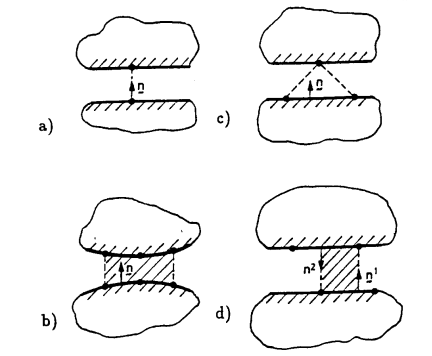
\includegraphics[scale=0.7]{Figure2/Chap4/abcd.png}
    \caption{Different contact discretizations}
    \label{fig:abcd}
\end{figure}
\subsection{Node–to–node Contact Element}
Figure \ref{fig:abcd} a) shows the so-called node–to–node contact which can only be applied to geometrically linear problems since a relative tangential movement of the nodes is not allowed in
the contact area. Due to its simplicity it resolves the integral (\ref{eqn:4.32}) to
\begin{equation}
 \int_{\Gamma_{c}} \epsilon_{N} g_{N} \delta g_{N} d \Gamma \longrightarrow \sum_{i=1}^{n_{c}} \epsilon_{N} g_{N i} \delta g_{N i} A_{i}=\sum_{i=1}^{n_{c}} \epsilon_{N} g_{N i}\left(\boldsymbol{\eta}_{i}^{1}-\boldsymbol{\eta}_{i}^{2}\right) \cdot \mathbf{n}_{i}^{2} A_{i} 
 \label{eqn:4.46}
\end{equation}

where $n _c$ are the contact nodes in $\Gamma^h_c$. The test function $\eta_i^\alpha$ and the normal vector $n^ 2_ i$ is
defined for the node $i$ . Often the area $A_ i$ is neglected
(or ”hidden” in the penalty parameter - $\epsilon_N$ ) in the node–to–node contact formulation which
means that the contact stress $p_N=\epsilon_N g_N$ becomes a contact (nodal) force $f_{Ni}=\epsilon_N g_{Ni}$ .Then an evaluation of a contact interface law is not possible with discretization
(\ref{eqn:4.46}). The associated matrix formulation leads in the geometrically linear case for the contact
element i to the definition of the contact residual $G ^c_i = \xi ^T G^ c_i $ and its associated tangent
matrix $K ^c_i $ with
\begin{equation}
 \mathbf{G}_{i}^{c}=\epsilon_{N} g_{N i} \mathbf{N}_{i}, \quad \mathbf{K}_{i}^{c}=\epsilon_{N} \mathbf{N}_{i} \mathbf{N}_{i}^{T}, \quad  \textit{with}  \quad \mathbf{N}_{i}=\left\{\begin{array}{r}\mathbf{n}_{i}^{2} \\ -\mathbf{n}_{i}^{2}\end{array}\right\} 
\end{equation}

\subsection{Isoparametric Discretization of the Contact Contribution}
In Figure \ref{fig:abcd} b) a contact element is shown which also does not allow a relative tangential
movement in the contact area and thus is only valid for geometrically linear applications.
Within this element the gap function $g_{N+}$ is discretized by an isoparametric interpolations
leading also to a well defined contact pressure. We obtain with the interpolation
\begin{equation}
     g_{N+}^{h}=\sum_{I} N_{I}(\xi) g_{N I} \qquad  \textit{and}  \qquad \delta g_{N+}^{h}=\sum_{I} N_{I}(\xi)\left(\boldsymbol{\eta}_{I}^{1}-\boldsymbol{\eta}_{I}^{2}\right) \cdot \mathbf{n}^{2} 
\end{equation}
the discretization of the contact integral (\ref{eqn:4.32})
\begin{equation}
 \int_{\Gamma_{c}} \epsilon_{N} g_{N} \delta g_{N} d \Gamma \longrightarrow \int_{-1}^{1} \epsilon_{N} g_{N+}^{h}(\xi)\left[\sum_{I} N_{I}(\xi)\left(\boldsymbol{\eta}_{I}^{1}-\boldsymbol{\eta}_{I}^{2}\right) \cdot \mathbf{n}^{2}\right]\left\|\frac{d x^{h}}{d \xi}\right\| d \xi 
 \label{eqn:4.48}
\end{equation}

Finally numerical integration can be applied to evaluate (48). For the proper choice of the
numerical integration rule. This discretization leads to a contact element which
can be applied together with four or nine node quadilaterals for the continuum problem.
Due to the smooth discretization a good approximation of the contact pressure is obtained.
%-----------------------------------------------------------
\subsection{Node–to–segment Contact Discretization}
A more general discretization of the contact interface which allows also for large tangential
sliding is given by the setup depicted in Figure \ref{fig:abcd} c). This discretization is named node–to–segment contact element and is widely used in nonlinear finite element simulations of
contact problems.

Due to its importance we like to consider this contact element in more detail. Assume
that the discrete slave point (s) comes into contact with the master segment (1)–(2), see
Figure 6. With the interpolation for the master segment
\begin{equation}
 \hat{\mathbf{x}}^{2}(\xi)=\mathbf{x}_{1}^{2}+\left(\mathbf{x}_{2}^{2}-\mathbf{x}_{1}^{2}\right) \xi 
 \label{eqn:4.49}
\end{equation}
one can easily compute the tangent vector of the segment leading to
\begin{equation}
 \overline{\mathbf{a}}_{1}^{2}=\hat{\mathbf{x}}^{2}(\xi)_{, 1}=\left(\mathbf{x}_{2}^{2}-\mathbf{x}_{1}^{2}\right) 
 \label{eqn:4.50}
\end{equation}

It is connected to an orthonormal base vector $a ^2_1$  by $a ^2_1 = \overline{a}^2_1 / l $ with $l =\left\| x ^2_2 -  x ^2_1 \right\| $  being
the current length of the master segment. With the unit tangent vector $a ^2_1$ the unit normal
to the segment $(1)–(2)$ can be defined as $n ^2 = e _3 × a ^2_1$ .
\begin{figure}[H]
    \centering
    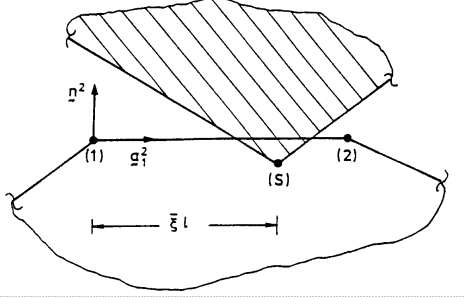
\includegraphics[scale=0.6]{Figure2/Chap4/fig6.png}
    \caption{Node–to–segment element}
    \label{fig4:6}
\end{figure}

$\overline{\xi}$ and $g _N$ are given by the solution of the minimal distance problem by the projection
of the slave node $x_s$ in $(s)$ onto the master segment $(1)–(2$)
\begin{equation}
    \label{eqn:4.51}
     \bar{\xi}=\frac{1}{l}\left(\mathbf{x}_{s}^{1}-\mathbf{x}_{1}^{2}\right) \cdot \mathbf{a}_{1}^{2} \quad  \textit{and}  \quad g_{N s}=\left\|\mathbf{x}_{s}^{1}-(1-\bar{\xi}) \mathbf{x}_{1}^{2}-\bar{\xi} \mathbf{x}_{2}^{2}\right\| 
\end{equation}

From these equations and the local formulation (\ref{eqn:4.4}) we compute directly the variation of the
gap function $\delta^g_{N+}$ on the straight master segment (1)–(2).
\begin{equation}
 \delta g_{N s}=\left[\boldsymbol{\eta}_{s}^{1}-(1-\bar{\xi}) \boldsymbol{\eta}_{1}^{2}-\bar{\xi} \boldsymbol{\eta}_{2}^{2}\right] \cdot \mathbf{n}^{2}
 \label{eqn:4.52}
\end{equation}

The local equation (\ref{eqn:4.9}) yields the expression for $\delta \overline{\xi}$.  With the interpolation for the variation $\hat{\boldsymbol{\eta}}^{2}(\xi)=\boldsymbol{\eta}_{1}^{2}+\xi\left(\boldsymbol{\eta}_{2}^{2}-\boldsymbol{\eta}_{1}^{2}\right) $ on the straight master segment $(1)–(2) $ we specialize
\begin{equation}
 \begin{aligned} \bar{H}_{\alpha \beta} &=\left(a_{\alpha \beta}+g_{N} b_{\alpha \beta}\right) \Longrightarrow \bar{H}_{11}=a_{11}=l^{2} \\ \bar{R}_{1} &=\left[\boldsymbol{\eta}^{1}-\hat{\boldsymbol{\eta}}^{2}(\bar{\xi})\right] \cdot \overline{\mathbf{a}}_{1}^{2}+g_{N s} \overline{\mathbf{n}}^{2} \cdot \hat{\boldsymbol{\eta}}_{1}^{2}(\bar{\xi}) \end{aligned} 
\end{equation}
which leads to
\begin{equation}
 \delta g_{T}=l \delta \bar{\xi}=\left[\boldsymbol{\eta}_{s}^{1}-(1-\bar{\xi}) \boldsymbol{\eta}_{1}^{2}-\bar{\xi} \boldsymbol{\eta}_{2}^{2}\right] \cdot \mathbf{a}_{1}^{2}+\frac{g_{N s}}{l}\left[\boldsymbol{\eta}_{2}^{2}-\boldsymbol{\eta}_{1}^{2}\right] \cdot \mathbf{n}^{2} 
\label{eqn:4.53}
\end{equation}

Equations (\ref{eqn:4.51}), (\ref{eqn:4.52}) and (\ref{eqn:4.53}) characterize the main kinematical relations of the contact
element in Figure \ref{fig:abcd} c).

In what follows we compute the contribution of the node–to–segment element to the weak
form (\ref{eqn:4.30}). The basic formulation for this discretization is analogous to (\ref{eqn:4.46}). Thus we assume
that we know the normal force $P _{N s} = p_ {N s} A_ s$ and the tangential force $T_{ T s} = t_ {T s} A _s$ at the
discrete contact point (s) of the contact element under consideration where A s denotes the
area of the contact element. Both forces, $P _{N s}$ and $ T_{Ts}$  leads to
\begin{equation}
 \int_{\Gamma_{c}}\left(p_{N} \delta g_{N}+t_{T} \delta g_{T}\right) d \Gamma-\longrightarrow \sum_{s=1}^{n_{c}}\left(P_{N s} \delta g_{N s}+T_{T s} \delta g_{T s}\right) 
 \label{eqn:4.54}
\end{equation}

 The contributions of one contact element in (\ref{eqn:4.54}) takes the form 
\begin{equation}
 \delta g_{N s} P_{N s}+\delta g_{T s} T_{T s} 
 \label{eqn:4.55}
\end{equation}
for the discrete contact point (s) with the mechanical relative (Lie–type) variations analogous
to (\ref{eqn:4.52}) and (\ref{eqn:4.53}). This equations can now be cast into a matrix formulation. For the normal
part $(\ref{eqn:4.54})_ 1$ we set for the variation (\ref{eqn:4.52}) of the penetration
\begin{equation}
 \delta g_{N s}=\mathbf{\eta}^{T} \mathbf{N}_{s} 
 \label{eqn:4.56}
\end{equation}

With the same notation we can express the variation (\ref{eqn:4.53}) of the tangential gap
\begin{equation}
    \delta g_{T s}=\boldsymbol{\eta}^{T}\left(\mathbf{T}_{s}+\frac{g_{N s}}{l} \mathbf{N}_{0 s}\right)
\label{eqn:4.57}
\end{equation}

In $ (\ref{eqn:4.56}) $ and $ (\ref{eqn:4.57}) $ the following vectors have been used
\begin{equation}
 \boldsymbol{\eta}=\left(\begin{array}{lll}\boldsymbol{\eta}_{s}^{1} & \boldsymbol{\eta}_{1}^{2} & \boldsymbol{\eta}_{2}^{2}\end{array}\right)^{T} 
 \label{eqn:4.58}
\end{equation}
% --cheater 
\begin{equation}
\label{eqn:4.59}
\mathbf{N}_{s}=\left\{\begin{array}{c}\mathbf{n}^{2} \\ -(1-\bar{\xi}) \mathbf{n}^{2} \\ -\bar{\xi} \mathbf{n}^{2}\end{array}\right\}, \quad
 \mathbf{N}_{0 s}=\left\{\begin{array}{c}\mathbf{0} \\ -\mathbf{n}^{2} \\ \mathbf{n}^{2}\end{array}\right\}_{s} 
\end{equation}
and
\begin{equation}
\label{eqn:4.60}
\mathbf{T}_{s}=\left\{\begin{array}{c}
\mathbf{a}_{1}^{2} \\
-(1-\bar{\xi}) \mathbf{a}_{1}^{2} \\
-\bar{\xi} \mathbf{a}_{1}^{2}
\end{array}\right\}, \quad \mathbf{T}_{0 s}=\left\{\begin{array}{c}
\mathbf{0} \\
-\mathbf{a}_{1}^{2} \\
\mathbf{a}_{1}^{2}
\end{array}\right\}
\end{equation}

Thus the virtual mechanical work $ (55) $ of the contact element can be written in the matrix formulation $ \boldsymbol{\eta}^{T} \mathbf{G}_{s}^{c} $ with the contact element residual
\begin{equation}
\label{eqn:4.61}
\mathbf{G}_{s}^{c}=P_{N s} \mathbf{N}_{s}+T_{T s}\left(\mathbf{T}_{s}+\frac{g_{N s}}{l} \mathbf{N}_{0 s}\right)
\end{equation}

Due to this approach a pure displacement formulation of the contact problem is possible by expressing $ P_{N s} $ either through (13) or (15) or by the penalty relation $ P_{N s}=\epsilon_{N} g_{N s} $. This is in contrast to the Lagrangian multiplier technique, where $ P_{N s}=\lambda_{N s} . $ But we observe that this discretization can be applied to both methods. In case of the augmented Lagrangian method we have to replace $ P_{N s} $ in $ (61) $ by
\begin{equation}
\label{eqn:4.62}
 P_{N s}^{\text {new }}=\bar{P}_{N s}^{o l d}+\epsilon_{N}\left\{g_{N s}^{n e w}-\left[\zeta-d\left(P_{N s}^{o l d}\right)\right]\right\} 
\end{equation}
 $ g_{N s} $ is given by $ (\ref{eqn:4.51}) $. 

Often a Newton-Raphson iteration is used to solve the global set of equations. Then the linearization of $ (\ref{eqn:4.61}) $ is needed to achieve quadratic convergence near the solution point. The associated derivation is a little bit cumbersome and thus only the final results will be summarized for this discretization. 

The tangent matrix for the normal contact is derived from the term $ \delta g_{N s} P_{N s}^{\prime} $ in $ (\ref{eqn:4.55}) $. Note that in $ (\ref{eqn:4.52}) $ the change in $ \bar{\xi} $ has be considered as well as the change of the normal $ \mathbf{n}^{2} $. For the penalty approach with $ P_{N s}=\epsilon_{N} g_{N s} $ we obtain the tangent matrix



$ \mathbf{K}_{N s}^{c}=\epsilon_{N}\left[\mathbf{N}_{s} \mathbf{N}_{s}^{T}-\frac{g_{N s}}{l}\left(\mathbf{N}_{0 s} \mathbf{T}_{s}^{T}+\mathbf{T}_{s} \mathbf{N}_{0 s}^{T}+\frac{g_{N s}}{l} \mathbf{N}_{0 s} \mathbf{N}_{0 s}^{T}\right)\right] $



The used matrices have been defined in $ (\ref{eqn:4.59}) $ and $ (\ref{eqn:4.60}) $. Note that in a geometrically linear case all terms vanish which are multiplied by $ g_{N s} . $ This gives the simple matrix $ \mathbf{K}_{N s}^{L c}=\epsilon_{N} \mathbf{N}_{s} \mathbf{N}_{s}^{T} $

For the tangential contributions in the contact area we have to linearize the term $ \delta g_{T s} T_{T s} $ in $ (\ref{eqn:4.55}) $.
\begin{equation}
 \label{eqn:4.64}   
 \begin{aligned} \mathbf{K}_{T s}^{c}=c_{T}\{&\left(\mathbf{T}_{s}+\frac{g_{N s}}{l} \mathbf{N}_{0 s}\right)\left(\mathbf{T}_{s}+\frac{g_{N s}}{l} \mathbf{N}_{0 s}\right)^{T} \\ &+\frac{g_{N s}}{l}\left[\mathbf{N}_{0 s} \mathbf{N}_{s}^{T}+\mathbf{N}_{s} \mathbf{N}_{0 s}^{T}-\mathbf{T}_{0 s} \mathbf{T}_{s}^{T}-\mathbf{T}_{s} \mathbf{T}_{0 s}^{T}\right.\\ &\left. \left.-2 \frac{g_{N s}}{l}\left(\mathbf{N}_{0 s} \mathbf{T}_{0 s}^{T}+\mathbf{T}_{0 s} \mathbf{N}_{0 s}^{T}\right)\right]\right\} \end{aligned} 
\end{equation}



Also in this case all terms containing $ g_{N s} $ disappear in a geometrically linear situation which yields $ \mathbf{K}_{T s}^{L c}=c_{T} \mathbf{T}_{s} \mathbf{T}_{s}^{T} . $ The case of frictional slip leads to an additional contribution in $ (\ref{eqn:4.64}) $ .
\subsection{ Discretization with Contact Segments}
The discretization of the contact interface by segments as described for the linear case in Simo, Wriggers, Taylor (1985) or for large deformations in Papadopoulos, Taylor (1992) leads to a special mixed formulation. Following Simo, Wriggers, Taylor (1985) we state the interpolation of the gap function $ g_{N} $ and its variation $ \delta g_{N} $ for a geometrically linear setting as follows

\begin{equation}
\label{eqn:4.65}
g_{N}=\left[\mathbf{u}^{1}(\xi)-\mathbf{u}^{2}(\xi)\right] \cdot \mathbf{n}(\xi) \quad \delta g_{N}=\left[\boldsymbol{\eta}^{1}(\xi)-\boldsymbol{\eta}^{2}(\xi)\right] \cdot \mathbf{n}(\xi)
\end{equation}

These interpolations are applied within a segement which is defined by the edge nodes $ \mathbf{x}_{2}^{A} $ and the projections onto the other surface $ \overline{\mathbf{x}}^{{A}} $, see Figure \ref{fig4:7}.
\begin{figure}
    \centering
    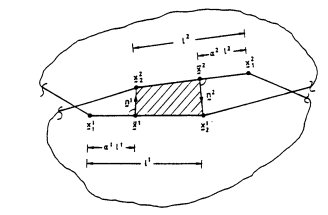
\includegraphics{Figure2/Chap4/fig7.png}
    \caption{Contact segment element}
   \label{fig4:7}
\end{figure}

Within this segment the displacement field and its variation is given as
\begin{equation}
\label{eqn:4.66}
\mathbf{u}^{\gamma}(\xi)=(1-\xi) \overline{\mathbf{u}}^{\gamma}+\xi \mathbf{u}_{2}^{\gamma} \quad \boldsymbol{\eta}^{\gamma}(\xi)=(1-\xi) \overline{\boldsymbol{\eta}}^{\gamma}+\xi \boldsymbol{\eta}_{2}^{\gamma}
\end{equation}
or the surface of the body $ \mathcal{B}^{\gamma}, \gamma=1,2 $. For the perturbed Lagrangian approach $ (38) $ the contact contributions take the form

\begin{equation}
\label{eqn:4.67}
\begin{aligned} \int_{\Gamma_{c}} \lambda_{N} \delta g_{N} d \Gamma &=\sum_{s=1}^{n_{s e g}} \int_{\Gamma_{s}} \lambda_{N} \delta g_{N} d \Gamma \\ \int_{\Gamma_{c}}\left(-\frac{\lambda_{N}}{\epsilon_{N}}+g_{N}\right) \delta \lambda_{N} d \Gamma &=\sum_{s=1}^{n_{s e g}} \int_{\Gamma_{s}}\left(-\frac{\lambda_{N}}{\epsilon_{N}}+g_{N}\right) \delta \lambda_{N} d \Gamma=0 \end{aligned} 
\end{equation}
where the latter equation can be solved for $ \lambda_{N} $ directly. With the interpolations $ (65) $ and assuming a constant contact pressure $ \lambda_{N} $ within the segment, $ \lambda_{N}=\bar{\lambda}_{N}=C O N S T . $, we obtain for the segment $ \Gamma_{s} $
\begin{equation}
\label{eqn:4.68}
\begin{aligned} \int_{\Gamma_{s}} \lambda_{N} \delta g_{N} d \Gamma &=\bar{\lambda}_{N} \int_{0}^{1}\left[\boldsymbol{\eta}^{1}(\xi)-\boldsymbol{\eta}^{2}(\xi)\right] \cdot \mathbf{n}(\xi)\left\|\frac{d \Gamma}{d \xi}\right\| d \xi \\ \int_{\Gamma_{s}}\left(-\frac{\lambda_{N}}{\epsilon_{N}}+g_{N}\right) \delta \lambda_{N} d \Gamma \Longrightarrow \bar{\lambda}_{N} &=\frac{\epsilon_{N}}{L_{s}} \int_{0}^{1}\left[\mathbf{u}^{1}(\xi)-\mathbf{u}^{2}(\xi)\right] \cdot \mathbf{n}(\xi)\left\|\frac{d \Gamma}{d \xi}\right\| d \xi \end{aligned}
\end{equation}
 The evaluation of these integrals by the trapezoidal rule yields the simple formulas
\begin{equation}
\begin{aligned}
\bar{\lambda}_{N} \int_{0}^{1}\left[\boldsymbol{\eta}^{1}(\xi)-\boldsymbol{\eta}^{2}(\xi)\right] \cdot \mathbf{n}(\xi)\left\|\frac{d \Gamma}{d \xi}\right\| d \xi & \approx \frac{1}{2} \bar{\lambda}_{N}\left(\left.\delta g_{N}\right|_{\xi=0}+\left.\delta g_{N}\right|_{\xi=1}\right) \\
\bar{\lambda}_{N} & \approx \frac{\epsilon_{N}}{2}\left(\left.g_{N}\right|_{\xi=0}+\left.g_{N}\right|_{\xi=1}\right)
\end{aligned}
\label{eqn:4.69}
\end{equation}
where $ g_{N} $ and $ \delta g_{N} $ can be expressed by the quantities in equations $ (\ref{eqn:4.65}) $ and $ (\ref{eqn:4.66}) $. This completes the discretization for contact segments. 


\subsection{ Global Set of Equations}
For a global algorithmic treatment we have to state the discrete set of equations. This leads for the penalty method to the general matrix formulation of the weak form
\begin{equation}
\mathbf{G}_{c}^{p}(\mathbf{v})=\mathbf{G}(\mathbf{v})+\cup_{s=1}^{n_{c}} \mathbf{G}_{s}^{c}(\mathbf{v})=\mathbf{0}
\label{eqn:4.70}
\end{equation}
where $ \mathbf{G}(\mathbf{v}) $ denotes the contributions of the bodies due to the weak form (43). In the second term $ s $ is associated with the active contact element, node or segment and $ \mathbf{G}_{s}^{c}(\varphi) $ has to be computed according to the chosen discretization, see previous sections. For the Lagrangian multiplier method the set of equations yields
\begin{equation}
\begin{array}{l}
\mathbf{G}_{c}^{1}(\mathbf{v}, \boldsymbol{\lambda})=\mathbf{G}(\mathbf{v})+\cup_{s=1}^{n_{c}} \mathbf{C}_{s}^{l}(\mathbf{v})^{T} \lambda_{s}=\mathbf{0} \\
\mathbf{G}_{c}^{2}(\mathbf{v}, \boldsymbol{\lambda})=\quad \cup_{s=1}^{n_{c}} \mathbf{C}_{s}^{g}(\mathbf{v}) \quad=\mathbf{0}
\end{array}
\label{eqn:4.71}
\end{equation}

Here the matrix $ C_{s}^{l}(\mathbf{v}) $ is related to the variation of $ \delta g_{s} $, see e.g. $ (\ref{eqn:4.68})_{1} $, and $ \mathbf{C}_{s}^{g}(\mathbf{v}) $ denotes the matrix formulation of the gap function $ g_{s} $ itself, see e.g. $ (\ref{eqn:4.68})_{2} $. These matrices also depend on the chosen discretization and are ment to contain not only the terms of the normal contact as indicated in (\ref{eqn:4.68}) but also the terms due to friction.

In case that Newton type methods are employed to solve $ (\ref{eqn:4.70}) $ or $ (\ref{eqn:4.71}) $ a linearization of the discrete set of equations has to be performed. Especially in the large deformation case the change in the normal has to be taken into account. 
\section{ ALGORITHMS FOR CONTACT PROBLEMS}

In this section we consider the algorithms which are essential for the treatment of contact problems. In general we have to distinguish between global algorithms which are necessary to find the correct number of active constraint equations and local algorithms which are needed to update contact stresses within the constitutive equations in the interface. Furthermore, also algorithms have to be deviced for coupled problems which may be necessary in case of thermomechanical coupling or for fluid-structure interaction problems.

The bandwidth of the global algorithms for constraint optimization is very broad. We like to mention, see also the introductory remarks, the simplex method, active set strategies, sequential quadratic programming, penalty and augmented Lagrangian techniques as well as barrier methods. All these techniques have advantages and disadvantages concerning efficiency, accuracy or robustness and thus have to be applied according to the problem
at hand. Algorithms for coupled problems, like staggered schemes, depend on the type of coupling and thus have to be designed with special care regarding robustness and efficiency. In the following we will sketch some of the global algorithms which are mainly applied to contact problems.

The update algorithms for the contact stresses, especially the tangential stresses due to friction, have been settled. In this case the so called projection methods or return mapping schemes yield the most efficient and robust treatment. Due to the fact that a algorithmic tangent operator can be constructed this technique can be incorporated in a Newton-Raphson scheme.

\subsection{ Global Algorithms}

The algorithm which is applied in many standard finite element programs is related to the penalty method. This is mainly due to its simplicity and furthermore it yields for many applications a robust algorithm. The penalty method is mostly combined with an active set strategy. The global set of equations is given in $ (\ref{eqn:4.70}) $. Now the algorithm for the penalty method can be summarized in here \\
\begin{framed}
Initialize algorithm \\
\ set: $ \mathbf{v}_{1}=\mathbf{0}, \quad \epsilon_{N}=\epsilon_{0} $\\
\hspace*{6mm} LOOP over iterations: $ i=1, \ldots $, convergence \\
\hspace*{10mm} Check for contact: $ g_{N s_{i}} \leq 0 \rightarrow $ active node, segment or element \\
 \hspace*{10mm} Solve: $ \mathbf{G}_{c}\left(\mathbf{v}_{i}\right)=\mathbf{G}\left(\mathbf{v}_{i}\right)+\cup_{s=1}^{n_{c}} \mathbf{G}_{s}^{c}\left(\mathbf{v}_{i}\right)=\mathbf{0} $ \\
 \hspace*{10mm} Check for convergence: $ \left\|\mathbf{G}_{c}\left(\mathbf{v}_{i}\right)\right\| \leq T O L \Rightarrow $ END LOOP \\
\hspace*{6mm}  END LOOP 
\\ update penalty parameter: $ \epsilon_{N} $
\end{framed}


Usually the solution of $ \mathbf{G}_{c}(\mathbf{v})=\mathbf{0} $ is performed by a Newton-Raphson iteration leading to
\begin{equation}
\label{eqn:4.72}
\begin{aligned}
D \mathbf{G}_{c}\left(\mathbf{v}_{i}^{n}\right) \Delta \mathbf{v}_{i}^{n+1} &=-\mathbf{G}_{c}\left(\mathbf{v}_{i}^{n}\right) \\
\mathbf{v}_{i}^{n+1} &=\mathbf{v}_{i}^{n}+\Delta \mathbf{v}_{i}^{n+1}
\end{aligned}
\end{equation}

where the operator $ D $ denotes the directional derivative of the vector $ \mathbf{G}_{c}\left(\mathbf{v}_{i}^{n}\right) $ which results in the tangent matrix $ \mathbf{K}_{T}\left(\mathbf{v}_{i}^{n}\right)=D \mathbf{G}_{c}\left(\mathbf{v}_{i}^{n}\right) $. The iteration index $ n $ is related to the Newton loop to solve $ \mathbf{G}_{c}\left(\mathbf{v}_{i}\right)=\mathbf{0} $ in Box 1 . Often the active set strategy, stated in Box 1, is accelerated in such a way that the update of the active set of contact constraints is performed within each step in the Newton iteration. Then the iteration $ (72) $ yields
\begin{equation}
\label{eqn:4.73}
 \begin{aligned} D \mathbf{G}_{c}\left(\mathbf{v}_{i}\right) \Delta \mathbf{v}_{i+1} &=-\mathbf{G}_{c}\left(\mathbf{v}_{i}\right) \\ \mathbf{v}_{i+1} &=\mathbf{v}_{i}+\Delta \mathbf{v}_{i+1} \end{aligned} 
\end{equation}
which is considerably faster. However this procedure might not converge for all cases and thus has to be applied with care.

Within this algorithm, an increase of the penalty parameter is necessary when the final result shows visible penetrations and thus does not fulfill the constraint equation $ g_{n+}=0 $ in a correct way. On the other hand a penalty parameter which has been chosen
too large can lead to ill-conditioning of the equation system and thus has to be reduced to avoid this. On possibility for the choice of $ \epsilon_{N} $ is to relate the penalty parameter to the bulk modulus of the contacting bodies. However, since it is quite hard to estimate the penalty parameter for all cases it makes sense to apply the augmented Lagrangian technique.

Augmented Lagrangian technique are usually applied together with Uzawa type algorithms, see Bertsekas (1984), Glowinski, Le Tallec (1984) or Laursen, Simo (1991), which lead to an inner loop for the contact and an outer loop for the update of the Lagrangian parameters.



Let us remark that it is standard practice in augmented Lagrangian iterations also to update the penalty number $ \epsilon_{N} $ in order to obtain good convergence, see Bertsekas (1984). This is due to the fact that a small penalty parameter leads to very slow convergence since the update formula (42) is of first order and the contact forces due to the penalty are small. Thus it makes sense to increase the penalty parameter within a contact element $ s $ according to an update scheme, see Bertsekas (1984). Here we like to show this approach for the augmented Lagrangian scheme in combination with constitutive interface laws like (13). The update scheme yields
\begin{equation}
\label{eqn:4.74}
 \epsilon_{N s n+1}=\left\{\begin{array}{ll}10 \cdot \epsilon_{N s n} & \text { for }\left[c_{+}\left(\mathbf{V}_{s}, \bar{P}_{N s}\right)\right]_{n+1}>\frac{1}{4} \cdot\left[c_{+}\left(\mathbf{V}_{s}, \bar{P}_{N s}\right)\right]_{n} \text { and } \epsilon_{N s n} \leq \frac{k}{\sqrt{N t}} \\ \epsilon_{N s n} & \text { for }\left[c_{+}\left(\mathbf{V}_{s}, \bar{P}_{N s}\right)\right]_{n+1} \leq \frac{1}{4} \cdot\left[c_{+}\left(\mathbf{V}_{s}, \bar{P}_{N s}\right)\right]_{n}\end{array}\right. 
\end{equation}

In relation (\ref{eqn:4.74}) also a stopping criterion for the update of the penalty parameter has been introduced to avoid ill-conditioning. This is given by the estimate (39). The global augmented Lagrangian algorithm is shown in box bellow. Here we use again the discrete formulation (70) which has to be adjusted to incorporate the fixed Lagrangian parameters $ \bar{P}_{N s} $, see $ (62) $ for the node-to-segment discretization. By $ \cup_{s=1}^{n_{c}} \mathbf{G}_{s n+1}^{a}\left(\mathbf{v}, \bar{P}_{N s}\right) $ we denote the contribution of the fourth term in (41) for an active contact element $ s $.
\begin{framed}
    Initialize algorithm\\
    set: $ d_{0}=\xi, \quad \mathbf{v}=\mathbf{0}, \quad \bar{P}_{0}=0, \quad \epsilon_{N}=\epsilon_{N 0} $\\
LOOP over augmentations: $ n=1, . . $, convergence \\
\hspace*{6mm} LOOP over iterations : $ i=1, . . $  convergence\\
\hspace*{10mm} Solve: $ \mathbf{G}_{c}\left(\mathbf{v}_{i},\\ \bar{P}_{N_{n}}\right)=\mathbf{G}\left(\mathbf{v}_{i}\right)+\cup_{s=1}^{n_{c}} \mathbf{G}_{s n+1}^{a}=\mathbf{0} $\\
\hspace*{10mm} Check for convergence: $ \left\|\mathbf{G}_{c}\left(\mathbf{v}_{i}, \bar{P}_{N_{n}}\right)\right\| \leq T O L \Rightarrow $  END LOOP\\
\hspace*{6mm} END LOOP\\
\hspace*{6mm} LOOP over contact nodes : $s = 1,\dots, n_c$\\
\hspace*{10mm} Update: $\bar{P}_{N_{s} n+1}$ according to $(62)$ \\
\hspace*{10mm} Update: $d_{s n+1}=h\left(\bar{P}_{N_{s n+1}}\right)$ according to (12) \\
\hspace*{10mm} Update: $\epsilon_{N s n+1}$ according to $(74)$\\
\hspace*{10mm} Check for convergence: $ \frac{1}{\zeta}\left\|g_{N_{+}}\left(\mathbf{V}_{s i}\right)-\left(\zeta-d_{n+1}\right)\right\| \leq T O L \Rightarrow S T O P $\\
\hspace*{6mm} END LOOP\\
END LOOP \\ 
\end{framed}

% \input{Page/Chap4/29}
% \input{Page/Chap4/30}
%\chapter{Solving nonlinear contact examples using element 8-nodes} % Main chapter title

\label{Chapter4 } % For referencing the chapter elsewhere, use \ref{Chapter1} 

%----------------------------------------------------------------------------------------
In this chapter, we consider two examples that are Self-contact example and Rubber Blade
example.After calculating displacement and stress on the model, next we consider the result of
displacement at a specific point on the model and the maximum stress on the contact edge. All the
calculated results from MATLAB will be compared with the results obtained from ANSYS software.
\newpage
\section{Self-contact example}

\subsection{Requirements of the example}

The Figure \ref{fig:contactself_exam} shown the geometry of the Self-contact example.

\begin{figure}[H]
    \centering
    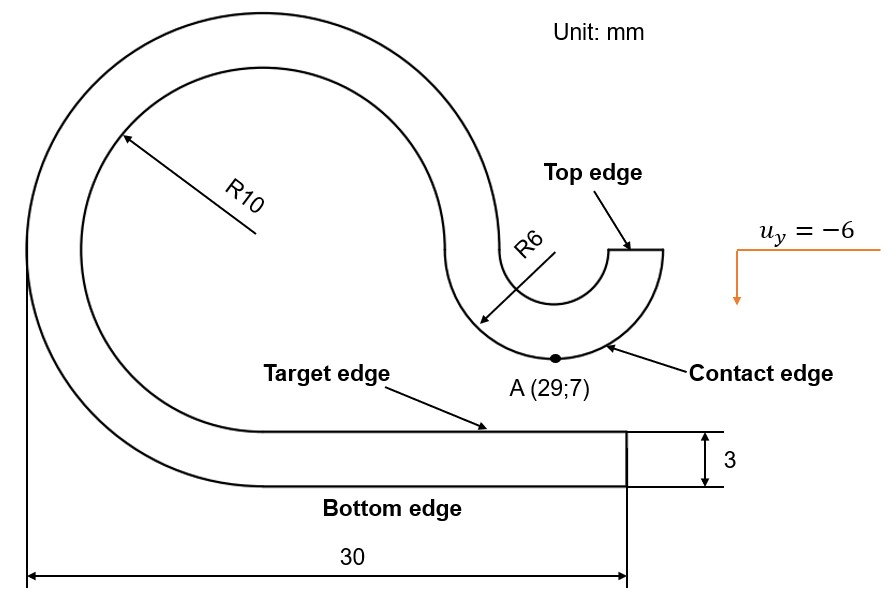
\includegraphics[scale=0.6]{Figures/contactself.jpg}
    \decoRule   
    \caption{Self-contact example}
    \label{fig:contactself_exam}
\end{figure} \noindent
\noindent
The model endures large deformation, when the deformation is large enough the
model will contact itself, technically called Self-contact. The model consists of the circle with
radius 10mm tangent to another circle with radius 6mm; below is Bottom edge which is fixed; above
is the Top edge which is applied displacement is $u_y = - 6 mm$. 
In this example the penalty method is applied to fulfill the contact constraint conditions.
Determine displacement and stress in the model.
Analysing displacement of {\bf point A} and maximal stress in {\bf contact edge} depends on
load step. \\

\newpage
\subsection{Preprocessor}
Element type: 8-nodes (Q8).
\vspace{0.38cm}
\newline
Material props: Neo-hookean model with material properties: the shear modulus ($\mu$) is assumed to 
be $80.194 N/mm^2$ and the bulk modulus ($\kappa$) is $120.291 N/mm^2$.
\vspace{0.38cm} \newline
Frictionless: in this study, contact problems with hyper-elastic materials are
considered in cases of frictionless sliding and frictionless compressing.
\vspace{0.38cm} \newline
Boundary conditions: in this example, we have the following boundary conditions: the Bottom edge is 
constrained displacement in the two directions x, y; Top edge is constrained to displacement in the 
x direction and is applied displacement is $u_y = - 6 mm$.
\vspace{0.38cm} \newline
Mesh: Figure \ref{fig:contactself_mesh_Q8} shown the mesh of the Self-contact example.
There is 357 total number of nodes, and 88 total number of elements.
\begin{figure}[H]
    \centering
    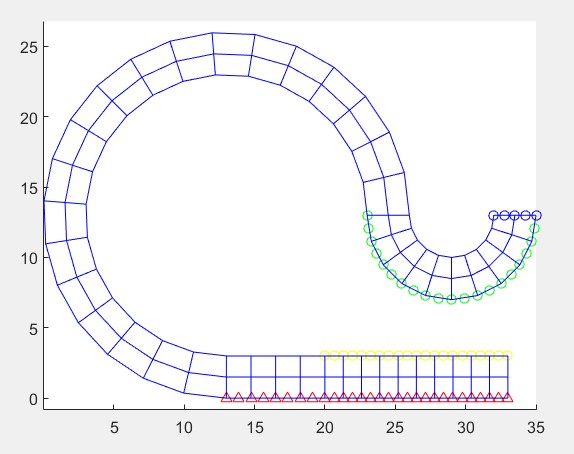
\includegraphics[scale=1]{Figures/contactself_mesh_Q8.jpg}
    \decoRule   
    \caption{Q8 mesh of Contact-self example}
    \label{fig:contactself_mesh_Q8}
\end{figure} \noindent \noindent
Number of steps: 60 steps and the convergence criterion is that of each step the residual force is less than 0.001.
\newpage

\subsection{Displacement}
\begin{figure}[H]
    \centering
    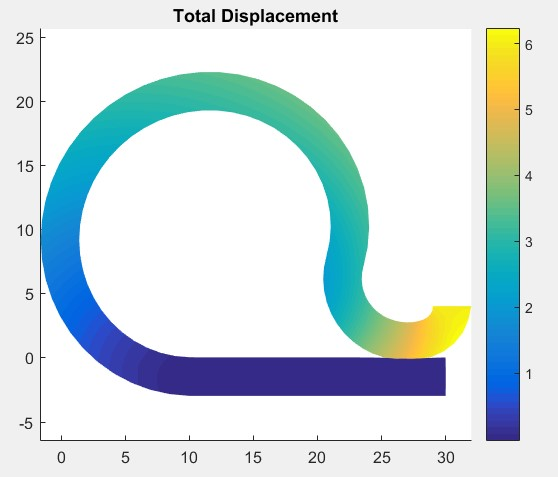
\includegraphics[scale=0.6]{Figures/t_displace_self_q8_matlab.jpg}
    \decoRule
    \caption{Total displacement of Contact-self example \\ (Q8 MATLAB)}
    \label{fig:t_displace_self_q8_matlab}
\end{figure} \noindent

\begin{figure}[H]
    \centering
    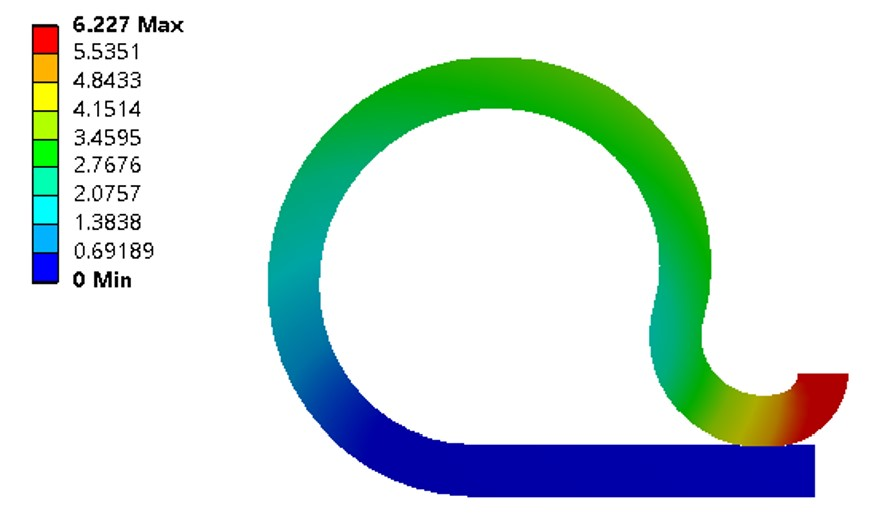
\includegraphics[scale=0.5]{Figures/t_displace_self_q8_ansys.jpg}
    \decoRule   
    \caption{Total displacement of Contact-self example \\ (Q8 ANSYS)}
    \label{fig:t_displace_self_q8_ansys}
\end{figure} \noindent
The total displacement is shown in the Figure \ref{fig:t_displace_self_q8_matlab}.
The Top edge is applied a vertical displacement -6 mm, so the contact edge is pressed down to the target edge. Because of the frictionless, the contact edge is not subsidence at the area where is contact with the target edge.
Then, the contact edge is sliced to the left side.
\vspace{0.38cm} \newline
The comparison of the total displacement between this study result and the reference result
is shown in the Figure \ref{fig:t_displace_self_q8_matlab} and Figure \ref{fig:t_displace_self_q8_ansys}.
So, there have not large difference between them.
The error of maximum total displacement between MATLAB solution and ANSYS solution is $0.1\%$
\newpage 
\noindent
To compare carefully, point A are considered in horizontal and vertical displacement. 
Figure \ref{fig:xA_displace_self_q8_matlab} shown the horizontal displacement of point A. 
Figure \ref{fig:yA_displace_self_q8_matlab} shown the vertical displacement of point A.
\vspace{0.38cm}
\begin{figure}[H]
    \centering
    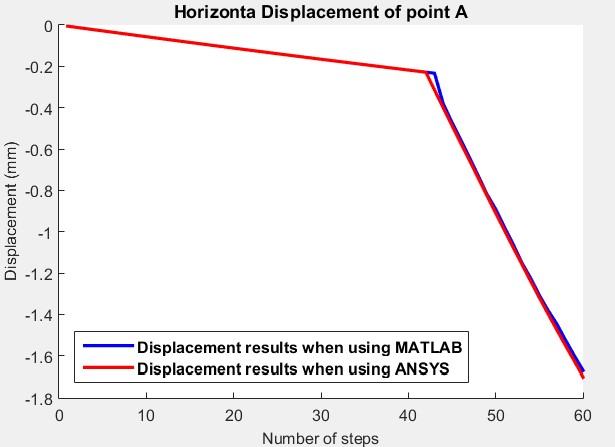
\includegraphics[scale=0.72]{Figures/xA_displace_self_q8_matlab.jpg}
    \decoRule
    \caption{Horizontal displacement of point A}
    \label{fig:xA_displace_self_q8_matlab}
\end{figure} \noindent.
\begin{figure}[H]
    \centering
    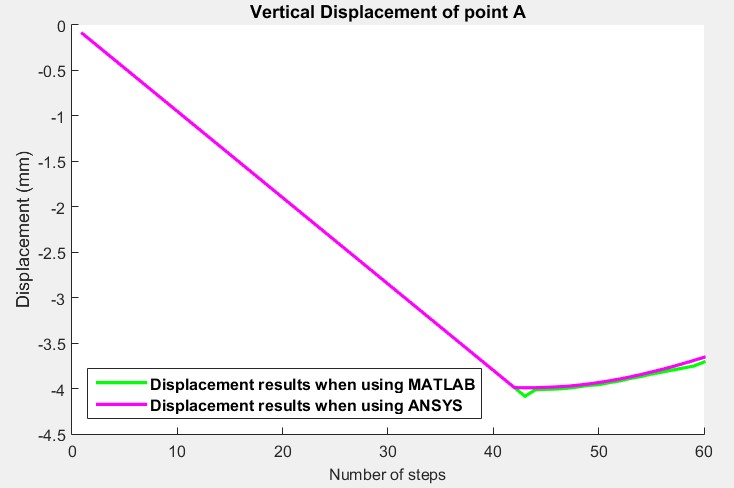
\includegraphics[scale=0.6]{Figures/yA_displace_self_q8_matlab.jpg}
    \decoRule
    \caption{Vertical displacement of point A}
    \label{fig:yA_displace_self_q8_matlab}
\end{figure} \noindent
At the point A, the displacement have a bit variability in load step 42.
Because here point A starts to touch the Target edge and 
there is a difference between how the problem is solved in the MATLAB program 
and in the ANSYS software.
\vspace{0.38cm} \newline
Follow Figure \ref{fig:xA_displace_self_q8_matlab}, we can see that 
the horizontal displacement of point A increases slowly before load step 42.
Before this load step, point A has not slipped on the Target edge.
After load step 42, point A slips on Target edge so horizontal displacement increases faster
\vspace{0.38cm} \newline
Follow Figure \ref{fig:yA_displace_self_q8_matlab}, we can see that
the vertical displacement of point A increases rapidly before load step 42,
then point A tends to go up.
Before this load step, point A has not slipped on the Target edge 
which means that point A is not obstructed in the vertical direction
After load step 42, point A slips on Target edge so point A can't go through the Target edge.
\subsection{Stress distribution}
\begin{figure}[H]
    \centering
    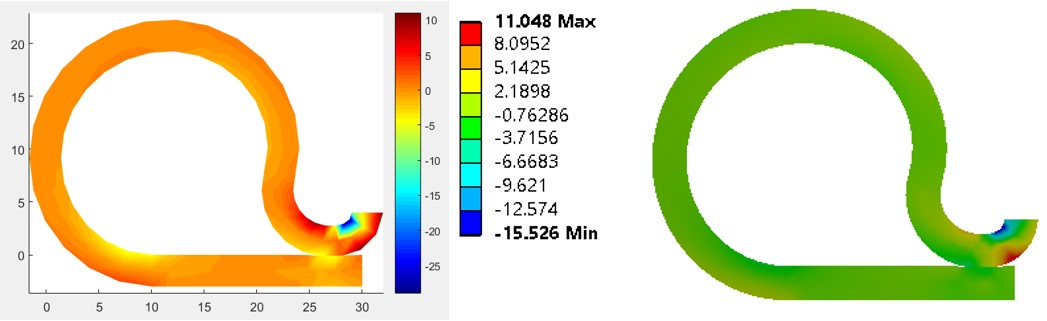
\includegraphics[scale=0.55]{Figures/sx_self_MandA.jpg}
    \decoRule
    \caption{Normal stress $\sigma_x$ of Contact-self example \\(MATLAB results on the left, ANSYS results on the right)}
    \label{fig:sx_self_MandA}
\end{figure} \noindent
Figure \ref{fig:sx_self_MandA} shown the normal stress $\sigma_x$ contour plot of the Contact-self example,
the left figure shown the contour plot of this study and the right one is the result of
commercial program (ANSYS). There are many stress concentration areas (compressive
stress and tensile stress), this figure also shown the comparison of the normal stress $\sigma_x$
distributions, it shown that the stress distributions are similar, 
so the normal stress $\sigma_x$ results can be acceptable.
Error of maximum normal stress $\sigma_x$ between MATLAB results and ANSYS is $1.13\%$
\\
\begin{figure}[H]
    \centering
    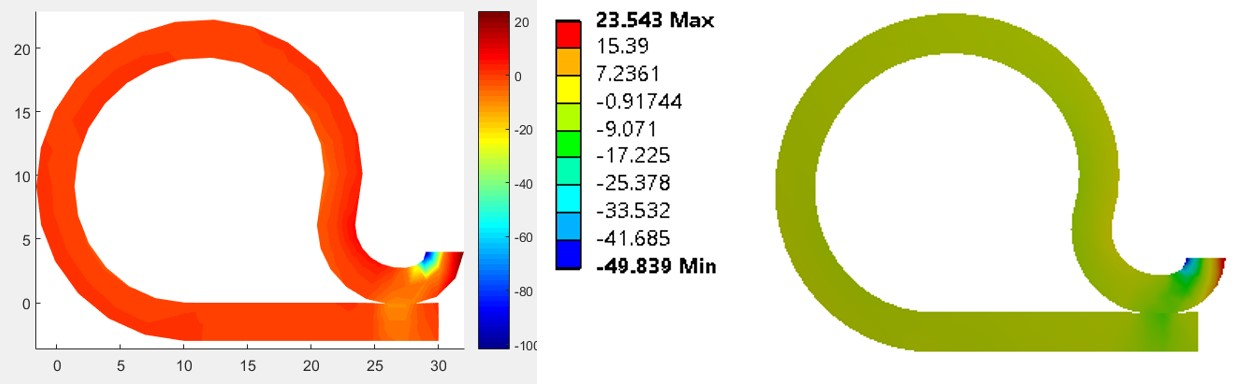
\includegraphics[scale=0.5]{Figures/sy_self_MandA.jpg}
    \decoRule
    \caption{Normal stress $\sigma_y$ of Contact-self example \\(MATLAB results on the left, ANSYS results on the right)}
    \label{fig:sy_self_MandA}
\end{figure} \noindent
Figure \ref{fig:sy_self_MandA} shown the normal stress $\sigma_y$ contour plot of the Contact-self example, 
the left figure shown the contour plot of this study and the right one is the result of commercial
program (ANSYS). Like Figure \ref{fig:sx_self_MandA},
from the results in the Figure \ref{fig:sy_self_MandA} there are many stress concentration areas (compressive and tensile stress),
it also shows a comparison of the normal stress $\sigma_y$ distributions,
showing that the stress distribution is similar,
since the result of normal stress $\sigma_y$ results is acceptable.
Error of maximum normal stress $\sigma_y$ between MATLAB results and ANSYS is $0.18\%$
\vspace{0.38cm} \newline
To specifically compare the variation of normal stress between MATLAB program and ANSYS software,
we consider the stress on contact edge under load strep.
Maximum stress in the contact edge is said to be an important component in the contact problem,
if the stress exceeds the allowable limit,
it is possible that on the contact edge, the model will be damaged.
\vspace{0.38cm} \newline
Maximum normal stress $\sigma_x$ and $\sigma_y$ of the contact edge will show in
Figure \ref{fig:sx_self_contact} and Figure \ref{fig:sy_self_contact}
\vspace{0.38cm}
\begin{figure}[H]
    \centering
    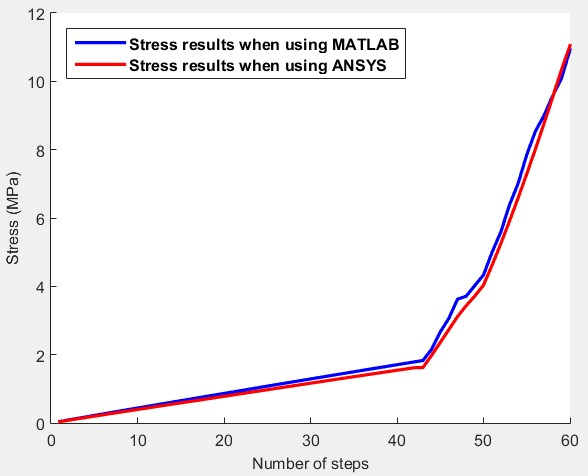
\includegraphics[scale=0.55]{Figures/sx_self_contact.jpg}
    \decoRule
    \caption{Normal stress $\sigma_x$ of contact edge}
    \label{fig:sx_self_contact}
\end{figure} \noindent

\begin{figure}[H]
    \centering
    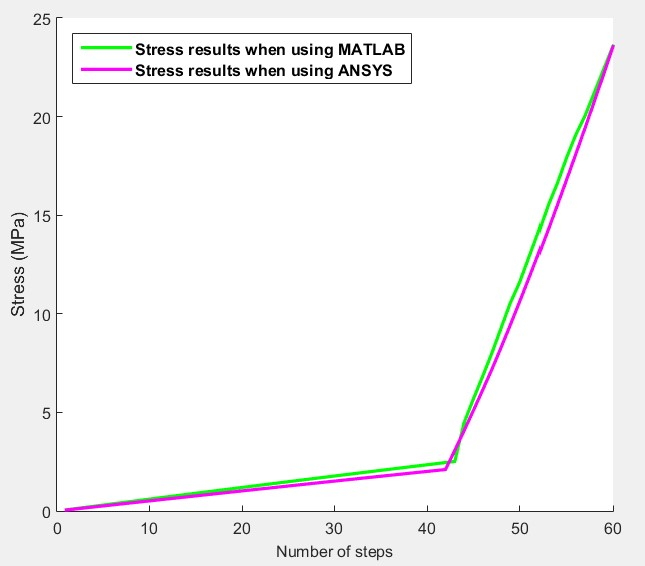
\includegraphics[scale=0.5]{Figures/sy_self_contact.jpg}
    \decoRule
    \caption{Normal stress $\sigma_y$ of contact edge}
    \label{fig:sy_self_contact}
\end{figure} \noindent
Look at Figure \ref{fig:sx_self_contact} and Figure \ref{fig:sy_self_contact},
we can see that the result of stress according to the load step 
between MATLAB results and ANSYS results is quite similar. Maximum normal stress $\sigma_x$ and maximum normal stress $\sigma_y$ both increase slowly before load step 42.
Since before this load step the Contact edge has not been in contact with the Target edge, the stress generated is mainly due to the deformation of the material.
After load step 42, the Contact edge contacts and slides on the Target edge; rapid increase in stress; In this stage, the stress generated is mainly due to the contact force between the upper part and the lower part.
Due to applied displacement in the y direction, the stress in the y direction is predominant and significantly larger than the stress in the x direction. 
\section{Rubber Blade example}
\subsection{Requirements of the example}
The Figure \ref{fig:model_rubber} shown the geometry of the Rubber Blade example
\begin{figure}[H]
    \centering
    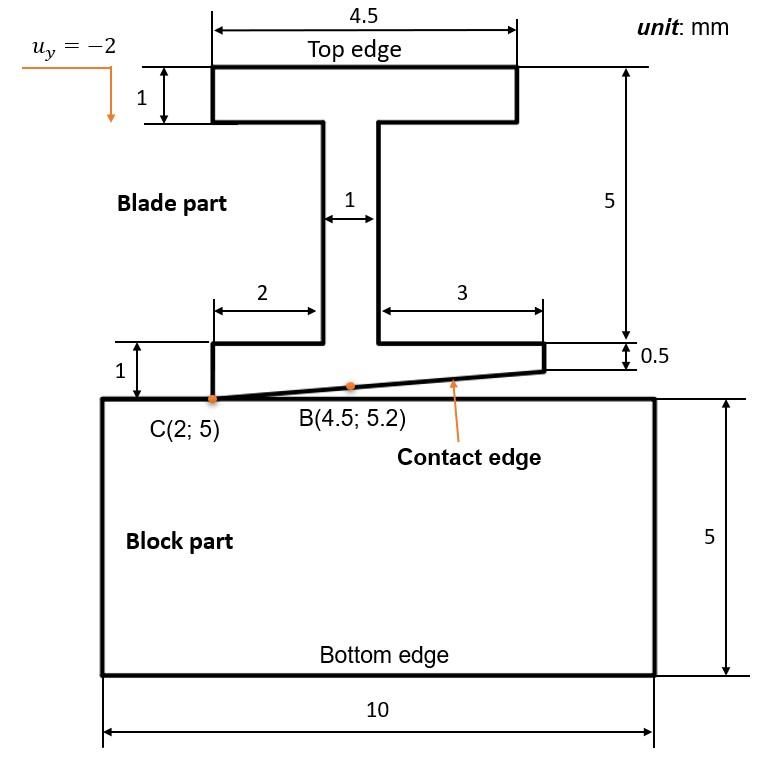
\includegraphics[scale=0.75]{Figures/model_rubber.jpg}
    \decoRule
    \caption{Rubber Blade example}
    \label{fig:model_rubber}
\end{figure}
\noindent
Different from Self-contact example, in this case, large sliding of the cross section of an elastic rubber blade is considered.
The rubber blade is subjected to a vertical prescribed displacement and pressed against a rubber block.
The contact is assumed to be frictionless.
In this example the penalty method is applied to fulfill the contact constraint conditions.
Determine displacement and stress in the model.
Analysing displacement of {\bf point B}, {\bf point C} and maximal stress in {\bf Contact edge} depends on load step.
\newpage
\subsection{Preprocessor}
Element type: 8-nodes (Q8).
\vspace{0.38cm} \newline
Material props: Neo-hookean model with material properties: the shear modulus ($\mu$) is assumed to 
be $80.194 N/mm^2$ and the bulk modulus ($\kappa$) is $60.291 N/mm^2$.
\vspace{0.38cm} \newline
Frictionless: in this study, contact problems with hyper-elastic materials are
considered in cases of frictionless sliding and frictionless compressing.
\vspace{0.38cm} \newline
Boundary conditions:
There is a vertical displacement applied in the top edge of the rubber blade. 
In this example, the vertical displacement is 2 mm. The contact areas are the bot edge of the rubber blade and the top edge of the block.
The block is fixed at the bottom.
\vspace{0.38cm} \newline
Mesh: Figure \ref{fig:mesh_rub} shown the mesh of the Self-contact example.
There is 435 total number of nodes, and 113 total number of elements.
\begin{figure}[H]
    \centering
    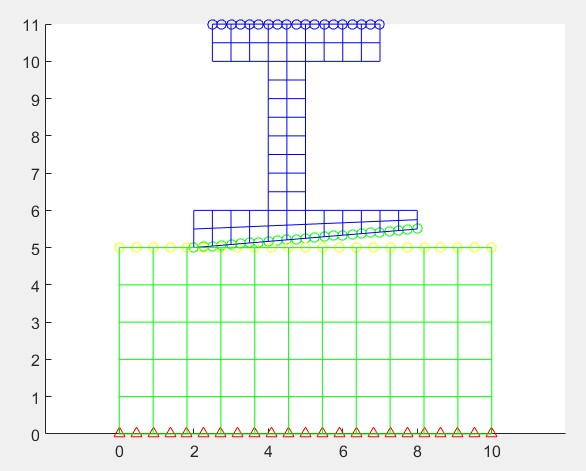
\includegraphics[scale=1]{Figures/mesh_rub.jpg}
    \decoRule
    \caption{Q8 mesh of Rubber Blade example}
    \label{fig:mesh_rub}
\end{figure} \noindent
Number of steps: 20 steps and the convergence criterion is that of each step the residual force is less than 0.001.
\newpage
\subsection{Displacement}
\begin{figure}[H]
    \centering
    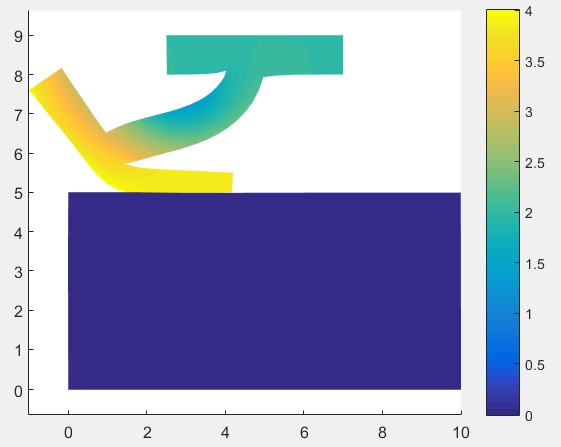
\includegraphics[scale=0.8]{Figures/dt_rub_mat.jpg}
    \decoRule
    \caption{Total displacement of rubber blade example (MATLAB)}
    \label{fig:dt_rub_mat}
\end{figure} \noindent
\begin{figure}[H]
    \centering
    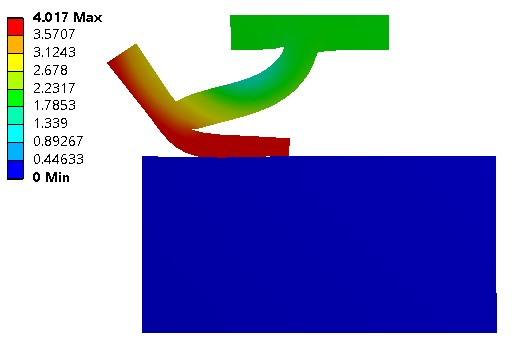
\includegraphics[scale=1]{Figures/dt_rub_an.jpg}
    \decoRule
    \caption{Total displacement of rubber blade example (ANSYS)}
    \label{fig:dt_rub_an}
\end{figure} \noindent
The total displacement is shown in the Figure \ref{fig:dt_rub_mat}. The blade is applied a vertical
displacement 2 mm, so the blade is pressed down to the block. Because of the frictionless,
the block is not subsidence at the area where is contact with the blade. Then, the bottom
side of the blade is sliced to the left side.
\vspace{0.38cm} \newline
The comparison of the total displacement between this study result and the reference result
is shown in the Figure \ref{fig:dt_rub_mat} and Figure \ref{fig:dt_rub_an}. So, there have not large difference between them. 
The error of maximum total displacement between MATLAB solution and ANSYS solution is $0.3\%$.
\vspace{0.38cm} \newline
To compare carefully, two points (B and C) are considered in vertical and horizontal displacement during load steps.
Figure \ref{fig:disB} shown the displacement of point B, and Figure \ref{fig:dc}  shown the displacement of point C.
\begin{figure}[H]
    \centering
    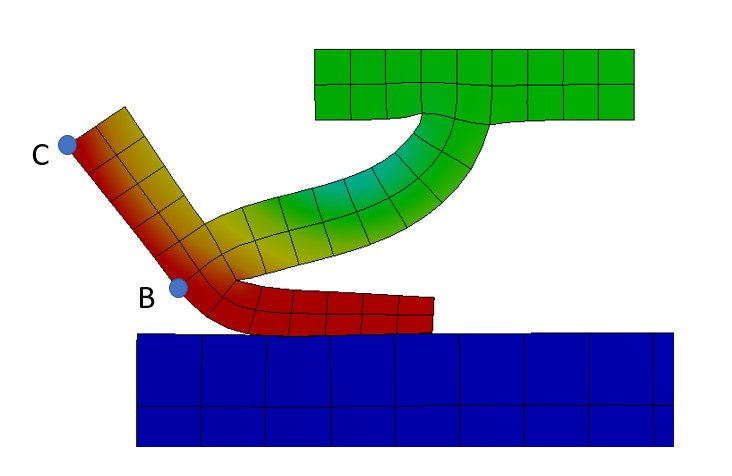
\includegraphics[scale=0.75]{Figures/dbdc.jpg}
    \decoRule
    \caption{Position of point B and C}
    \label{fig:dbdc}
\end{figure} \noindent
\begin{figure}[H]
    \centering
    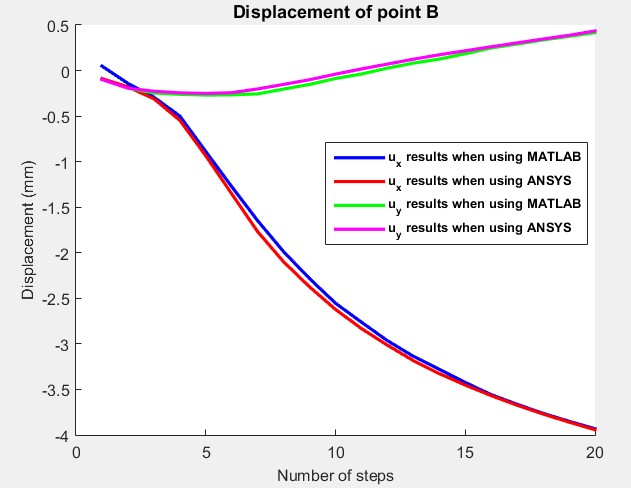
\includegraphics[scale=0.8]{Figures/disB.jpg}
    \decoRule
    \caption{Displacement of point B}
    \label{fig:disB}
\end{figure} \noindent
At the point B, the vertical displacement have a bit variability, because of the nonlinear
behavior of contact, at the beginning, the point A have to be moved a small distance (0 to
5 load step) to contact with the block.  After that, the point A moved up because the
contact reaction forces. Also after sliding on block part, contact edge tends to go up.
For the horizontal displacement, there is the rapid rise of the
displacement in load step 0 to 5, because point A has not been in contact with {\bf the block part}, then point A slides to the left at this time the horizontal displacement of point A increases rapidly.
\newline
\begin{figure}[H]
    \centering
    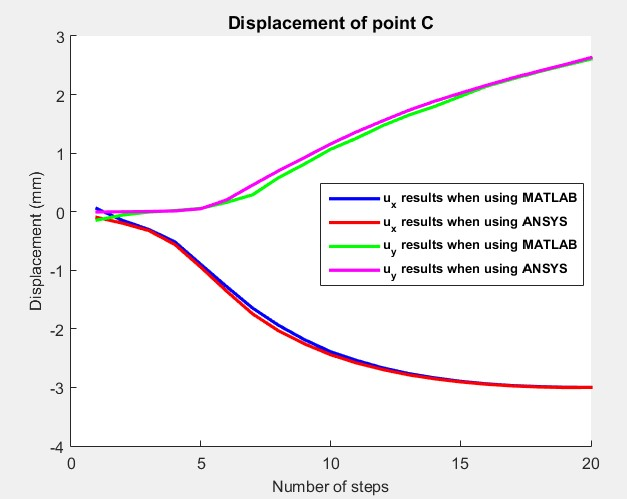
\includegraphics[scale=0.83]{Figures/dc.jpg}
    \decoRule
    \caption{Displacement of point B}
    \label{fig:dc}
\end{figure} \noindent
For the point C, the vertical displacement is almost the same as the point B, but there is no downward displacement stage. Vertical displacement slows up in the early stages, where point C just slipped off the block part. 
After about 7th load step, point C tends to go up due to the general deformation of the model.
For the horizontal displacement, there is a stage (load step 0 to 5) which increases slowly. Because in this stage the contact edge begins to approach the block part, the slip has not taken place much, so point C has a little horizontal displacement.
After 7th load step, contact edge completely slides on the block part, the slip has taken place much, point C moves left faster.
\newpage
\subsection{Stress distribution}
\begin{figure}[H]
    \centering
    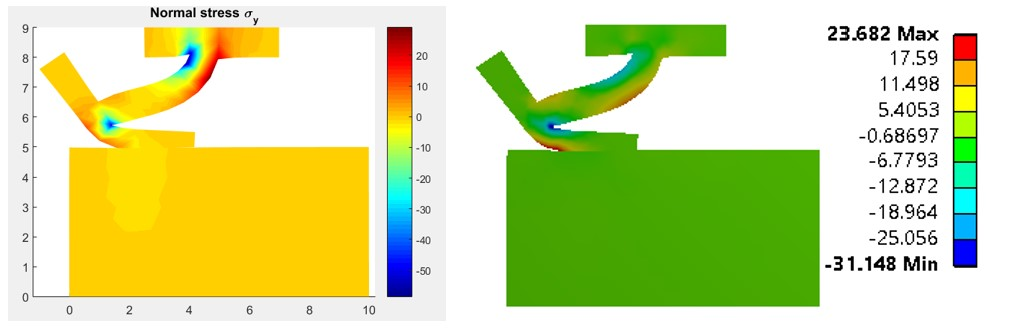
\includegraphics[scale=0.63]{Figures/sx_rub_MvsA.jpg}
    \decoRule
    \caption{Normal stress $\sigma_x$ of rubber blade example \\(MATLAB results on the left, ANSYS results on the right)}
    \label{fig:sx_rub_MvsA}
\end{figure} \noindent
Figure \ref{fig:sx_rub_MvsA} shown the normal stress $\sigma_x$ contour plot of the rubber blade example,
the left figure shown the contour plot of this study and the right one is the result of
commercial program (ANSYS). There are many stress concentration areas (compressive
stress and tensile stress), this figure also shown the comparison of the normal stress $\sigma_x$
distributions, it shown that the stress distributions are similar, so the normal
stress $\sigma_x$ results can be acceptable.
Error of maximum normal stress $\sigma_x$ between MATLAB results and ANSYS is $0.85\%$.
\newline
\begin{figure}[H]
    \centering
    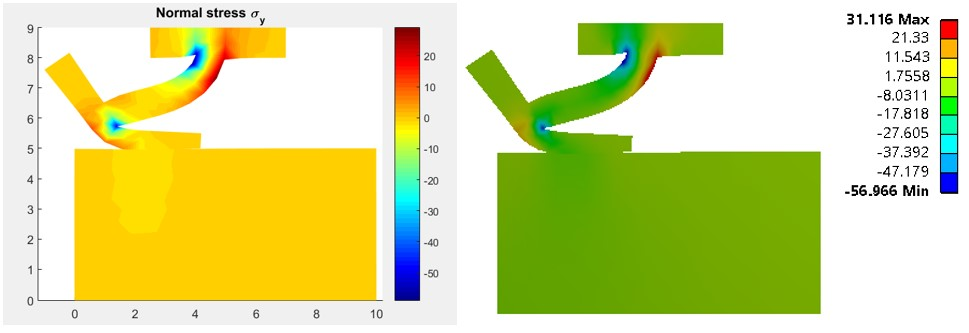
\includegraphics[scale=0.65]{Figures/sy_rub_MvsA.jpg}
    \decoRule
    \caption{Normal stress $\sigma_y$ of rubber blade example \\(MATLAB results on the left, ANSYS results on the right)}
    \label{fig:sy_rub_MvsA}
\end{figure} \noindent
\noindent
Figure \ref{fig:sy_rub_MvsA} shown the normal stress $\sigma_y$ contour plot of the rubber blade example, the
left figure shown the contour plot of this study and the right one is the result of commercial
program (ANSYS). Like Figure 4.6, there are also many stress concentration areas (compressive
stress and tensile stress). It shown that the stress distributions are similar, so the normal $\sigma_y$
stress results can be acceptable.
Error of maximum normal stress $\sigma_y$ between MATLAB results and ANSYS is $6.85\%$.
We can see that the error of maximum normal stress $\sigma_y$ is significant (greater than $5\%$).
It's very likely due to applied displacement is $u_y = - 2 mm$ in top edge leads to compression in the y-direction, the error is mainly in the y-direction.
\vspace{0.38cm}
\newline 
Different from self-contact example, rubber blade example has a larger normal stress error.
This is understandable as the rubber blade example model is more complex than the self-contact example model. The model has more stress concentrations areas (shown in Figure \ref{fig:s_tt}).
In addition, the contact area of the rubber blade example (line to line) is larger than the contact area of the self-contact example (nearly node to line).
Self-contact example model we have only one part and rubber blade example model we have tow parts that are in contact with each other.
Furthermore, we are using 8 node element, it is suitable for problems with curves model.
\begin{figure}[H]
    \centering
    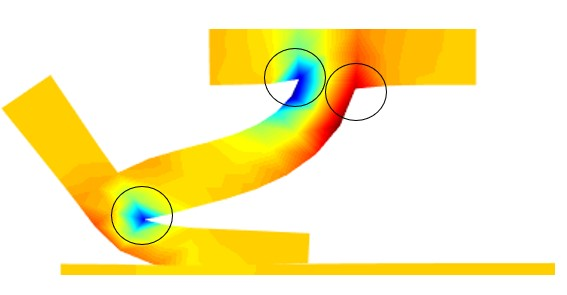
\includegraphics[scale=0.7]{Figures/s_tt.jpg}
    \decoRule
    \caption{Stress concentrations areas of rubber blade example}
    \label{fig:s_tt}
\end{figure} \noindent
To specifically compare the variation of normal stress between MATLAB program and ANSYS software,
we consider the stress on contact edge during load strep.
Maximum stress in the contact edge is said to be an important component in the contact problem,
if the stress exceeds the allowable limit,
it is possible that on the contact edge, the model will be damaged.
\vspace{0.38cm} \newline
Maximum normal stress $\sigma_x$ and $\sigma_y$ of the contact edge will show in
Figure \ref{fig:sx_c_r} and Figure \ref{fig:sy_c_r}
\newline
\begin{figure}[H]
    \centering
    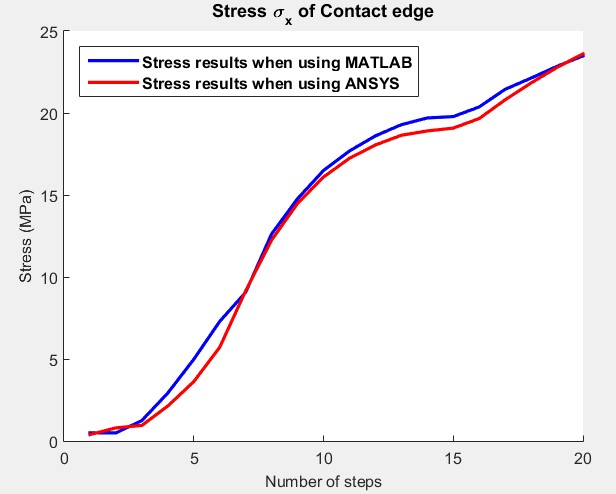
\includegraphics[scale=0.7]{Figures/sx_c_r.jpg}
    \decoRule
    \caption{Normal stress $\sigma_x$ of the contact edge}
    \label{fig:sx_c_r}
\end{figure} \noindent
Figure \ref{fig:sx_c_r} shown the comparison of the normal stress $\sigma_x$ in the contact edge during load step.
The shapes of twos curve are similar, but the values in many load step are different.
The reasons of this error are mesh quality, nonlinear behavior of large deformation and material and that may also be due to the difference between MATLAB and ANSYS solutions.
\vspace{0.38cm}
\begin{figure}[H]
    \centering
    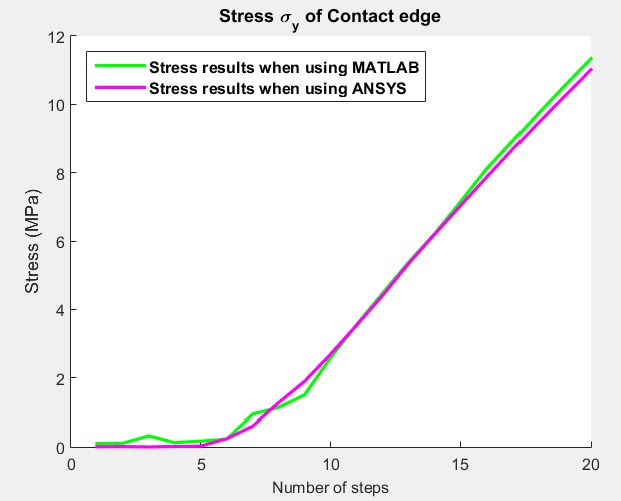
\includegraphics[scale=0.7]{Figures/sy_c_r.jpg}
    \decoRule
    \caption{Normal stress $\sigma_y$ of the contact edge}
    \label{fig:sy_c_r}
\end{figure} \noindent
Figure \ref{fig:sx_c_r} shown the comparison of the normal stress $\sigma_y$ in the contact edge during load step. Normal stress $\sigma_y$ increases rapidly after the 7th load step because the contact edge has made full contact with the block part.
The shapes of twos curve are similar, but the values in many load step are different. Same as normal stress $\sigma_x$,
the reasons of this error are mesh quality, nonlinear behavior of large deformation and material and that may also be due to the difference between MATLAB and ANSYS solutions.
\newline
\section{Discussion}
After solving two example problems, we can confirm that it is possible to apply the 8-nodes element to computational programming. With the computer increasingly upgraded in both hardware and software, the problem of the long solving time of the 8-nodes element has been overcome.
\vspace{0.38cm}
\newline
By solving the self-contact example, we can see that the 8-nodes element gives little error for the model with many curves.
The high order approximation for the finite element {\bf (keeping the same size)} leads to the small error for the solution. 
%\chapter{Compare element 8-nodes element 4-nodes in solving the contact examples} % Main chapter title

\label{Chapter5 } % For referencing the chapter elsewhere, use \ref{Chapter1} 
In this chapter, we re-solve two examples (self-contact example and rubber blade example) using 8-nodes and 4-nodes elements. The results calculated by the MATLAB program are compared with the results of the ANSYS software corresponding to the 8-nodes and 4-nodes elements (that is, the MATLAB calculation results of the 8-nodes element will be compared with the simulation results above. ANSYS software of the 8-nodes element, similarly for the 4-nodes element).
\vspace{0.38cm}
\newline
It makes no sense for us to compare 8-nodes element and 4-nodes element on the same element size. Thus, of course, using the 8-nodes element will give more accurate results. In this chapter, when using an element of 8-nodes, the size of the element will be four times larger than the size of a 4-nodes element (represented in the Figure \ref{fig:dif4-nodes8-nodes}).
\vspace{0.38cm}
\newline
Maximum volume displacement and maximum stress are compared in this chapter.
\newline
\begin{figure}[H]
    \centering
    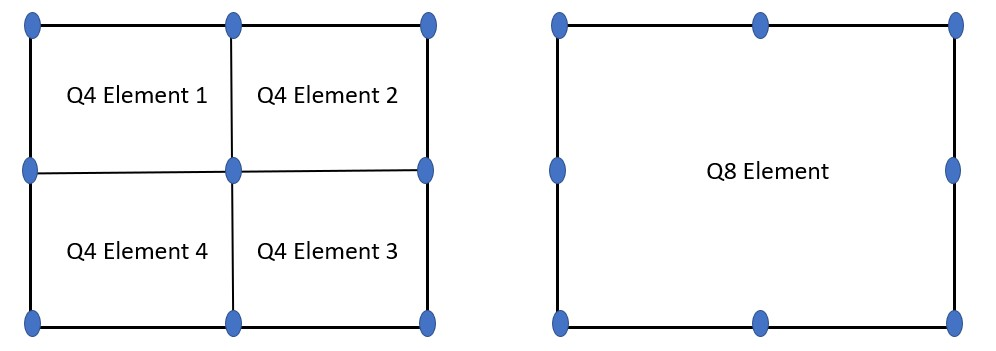
\includegraphics[scale=0.5]{Figures/chapter5/difQ4Q8.jpg}
    \decoRule
    \caption{Differences in meshing}
    \label{fig:dif4-nodes8-nodes}
\end{figure}
\newpage
\section{Self-contact example}
With the model and boundary conditions as in the previous chapter, we solve the problem using 8-nodes and 4-nodes elements.
\subsection{Mesh and solution time}
Material props: Neo-hookean model with material properties: the shear modulus ($\mu$) is assumed to be $80.194 N/mm^2$ and the bulk modulus ($\kappa$) is $120.291 N/mm^2$.
\vspace{0.38cm} \newline
Frictionless: in this study, contact problems with hyper-elastic materials are
considered in cases of frictionless sliding and frictionless compressing.
\vspace{0.38cm} \newline
Boundary conditions: in this example, we have the following boundary conditions: the Bottom edge is 
constrained displacement in the two directions x, y; Top edge is constrained to displacement in the 
x direction and is applied displacement is $u_y = - 6 mm$.
\vspace{0.38cm}
\newline
The case of meshing with 8-nodes is shown in Figure \ref{fig:q8_mesh_s}.
While for meshing with a 4-nodes element, it is shown in Figure \ref{fig:q4_mesh_s}.
Table \ref{tab:mp_s} shows the total number of nodes and the total number of elements of the model when meshing by two element types.
\vspace{0.01cm}
\newline

\begin{figure}[H]
    \centering
    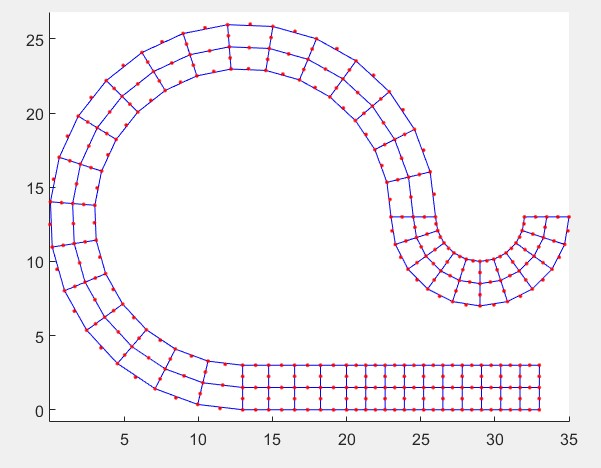
\includegraphics[scale=0.72]{Figures/chapter5/q8_mesh_s.jpg}
    \decoRule
    \caption{Mesh when using the 8-nodes element of self-contact example }
    \label{fig:q8_mesh_s}
\end{figure}

\begin{figure}[H]
    \centering
    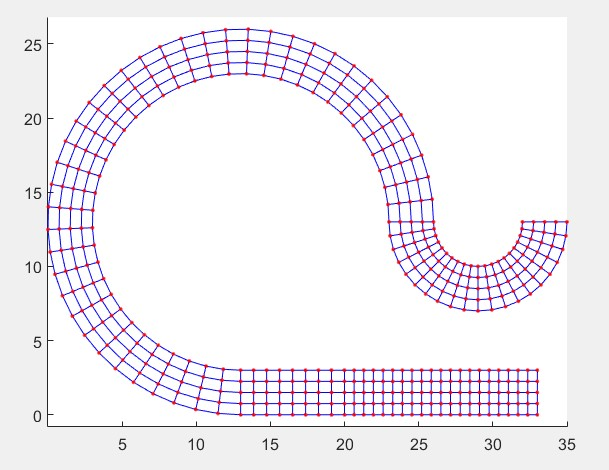
\includegraphics[scale=0.7]{Figures/chapter5/q4_mesh_s.jpg}
    \decoRule
    \caption{Mesh when using the 4-nodes element of self-contact example}
    \label{fig:q4_mesh_s}
\end{figure}
\begin{table}[H]
    \centering
    \scalebox{1}{
    \begin{tabular}{|c|c|c|}
    \multicolumn{3}{c}{Mesh properties} \\ \hline
         Element type & Total of node & Total of element \\ \hline 
         8-nodes      & 357        & 88 \\ \hline
         4-nodes      & 445        & 352 \\ \hline
    \end{tabular}}
    \caption{Mesh properties of self-contact example}
    \label{tab:mp_s}
\end{table}
\noindent
Although less in number of nodes and significantly less (four times) in number of elements, the solving time when using 8-nodes element is not much less than when using 4-nodes element.
The solving time is shown in the Table \ref{tab:st_s}
\begin{table}[H]
    \centering
    \begin{tabular}{|c|c|}
    \multicolumn{2}{c}{The solving time} \\ \hline
         Element type & Time \\ \hline 
         8-nodes           & 108s \\ \hline
         4-nodes           & 114s \\ \hline
    \end{tabular}
    \caption{The solving time of self-contact example}
    \label{tab:st_s}
\end{table}
\newpage
\subsection{Compare displacement}
%% COMPARE ux

% ux of q8
\begin{figure}[H]
    \centering
    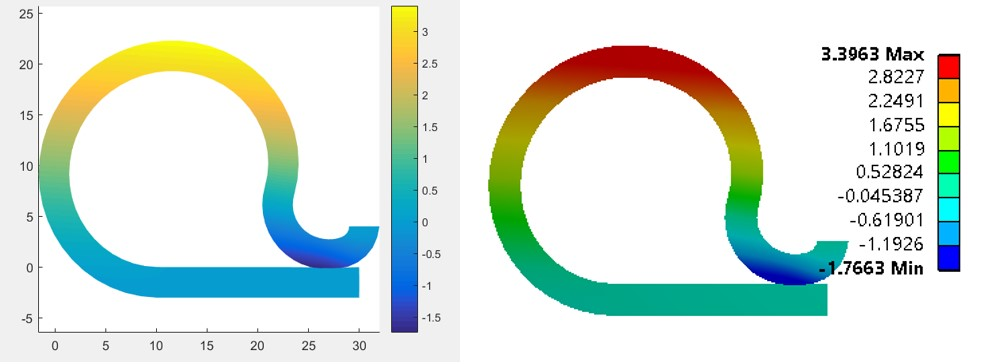
\includegraphics[scale=0.6]{Figures/chapter5/s_q8_ux.jpg}
    \decoRule
    \caption{$u_x$ displacement when using Q8 of self-contact example \\
    (MATLAB result in the left, ANSYS result in the right)}
    \label{fig:s_q8_ux}
\end{figure}
The $u_x$ displacement of self-contact example when using 8-nodes element is shown in the Figure \ref{fig:s_q8_ux}.
Maximum volume $u_x$ displacement of MATLAB result is $3.3923 mm$.
Maximum volume $u_x$ displacement of ANSYS result is $3.3963 mm$.
The error of maximum volume $u_x$ displacement between MATLAB result and ANSYS result when using 8-nodes element is $0.12\%$.
\newline

% ux of q4
\begin{figure}[H]
    \centering
    \includegraphics[scale=0.65]{Figures/chapter5/s_q4_ux.jpg}
    \decoRule
    \caption{$u_x$ displacement when using Q4 of self-contact example \\
    (MATLAB result in the left, ANSYS result in the right)}
    \label{fig:s_q4_ux}
\end{figure}
\noindent
The $u_x$ displacement of self-contact example when using 4-nodes element is shown in the Figure \ref{fig:s_q4_ux}.
Maximum volume $u_x$ displacement of MATLAB result is $3.3404 mm$.
Maximum volume $u_x$ displacement of ANSYS result is $3.3651 mm$.
The error of maximum volume $u_x$ displacement between MATLAB result and ANSYS result when using 4-nodes element is $0.73\%$.
So, for maximum volume $u_x$ displacement, the error when using 8-nodes element is lower than when using 4-nodes element.
\newpage
%% COMPARE uy
% uy of q8
\begin{figure}[H]
    \centering
    \includegraphics[scale=0.7]{Figures/chapter5/s_q8_uy.jpg}
    \decoRule
    \caption{$u_y$ displacement when using Q8 of self-contact example \\
    (MATLAB result in the left, ANSYS result in the right)}
    \label{fig:s_q8_uy}
\end{figure}
\noindent
The $u_y$ displacement of self-contact example when using 8-nodes element is shown in the Figure \ref{fig:s_q8_uy}.
Maximum volume $u_y$ displacement of MATLAB result is $6.2109mm$.
Maximum volume $u_y$ displacement of ANSYS result is $6.2159mm$.
The error of maximum volume $u_y$ displacement between MATLAB result and ANSYS result when using 8-nodes element is $0.08\%$.
\newline
% uy of q4
\begin{figure}[H]
    \centering
    \includegraphics[scale=0.66]{Figures/chapter5/s_q4_uy.jpg}
    \decoRule
    \caption{$u_y$ displacement when using Q4 of self-contact example \\
    (MATLAB result in the left, ANSYS result in the right)}
    \label{fig:s_q4_uy}
\end{figure}
\noindent
The $u_y$ displacement of self-contact example when using 8-nodes element is shown in the Figure \ref{fig:s_q4_uy}.
Maximum volume $u_y$ displacement of MATLAB result is $6.2132mm$.
Maximum volume $u_y$ displacement of ANSYS result is $6.2196mm$.
The error of maximum volume $u_y$ displacement between MATLAB result and ANSYS result when using 8-nodes element is $0.1\%$.
So, for maximum volume $u_y$ displacement, the error when using 8-nodes element is lower than when using 4-nodes element.
\vspace{0.38cm}
\newline
Thus, for the self-contact example, using the 8-nodes element gives more accurate displacement results than using the 4-nodes element.
\newpage
\subsection{Compare stress distribution}
%% COMPARE SX
% sx of q8
\begin{figure}[H]
    \centering
    \includegraphics[scale=0.575]{Figures/sx_self_MandA.jpg}
    \decoRule
    \caption{Normal stress $\sigma_x$ when using Q8 of self-contact example \\
    (MATLAB result in the left, ANSYS result in the right)}
    \label{fig:sx_self_MandA_5}
\end{figure}
\noindent
The normal stress $\sigma_x$ of self-contact example when using 8-nodes element is shown in the Figure \ref{fig:sx_self_MandA_5}.
Maximum normal stress $\sigma_x$ of MATLAB result is $10.9231 MPa$.
Maximum normal stress $\sigma_x$ of ANSYS result is $11.048 MPa$.
The error of maximum normal stress $\sigma_x$ between MATLAB result and ANSYS result when using 8-nodes element is $1.13\%$.
\newline
% sx of q4
\begin{figure}[H]
    \centering
    \includegraphics[scale=0.54]{Figures/chapter5/sx_q4_c.jpg}
    \decoRule
    \caption{Normal stress $\sigma_x$ when using Q4 of self-contact example \\
    (MATLAB result in the left, ANSYS result in the right)}
    \label{fig:sx_q4_c}
\end{figure}
\noindent
The normal stress $\sigma_x$ of self-contact example when using 4-nodes element is shown in the Figure \ref{fig:sx_q4_c}.
Maximum normal stress $\sigma_x$ of MATLAB result is $14.1402 MPa$.
Maximum normal stress $\sigma_x$ of ANSYS result is $15.204 MPa$.
The error of maximum normal stress $\sigma_x$ between MATLAB result and ANSYS result when using 8-nodes element is $7\%$.
So, for maximum normal stress $\sigma_x$, the error when using 8-nodes element is lower than when using 4-nodes element.
\newpage

%% COMPARE SY
% sx of q8
\begin{figure}[H]
    \centering
    \includegraphics[scale=0.5]{Figures/sy_self_MandA.jpg}
    \decoRule
    \caption{Normal stress $\sigma_y$ when using Q8 of self-contact example \\
    (MATLAB result in the left, ANSYS result in the right)}
    \label{fig:sy_self_MandA_5}
\end{figure}
\noindent
The normal stress $\sigma_y$ of self-contact example when using 8-nodes element is shown in the Figure \ref{fig:sy_self_MandA_5}.
Maximum normal stress $\sigma_y$ of MATLAB result is $23.5783 MPa$.
Maximum normal stress $\sigma_y$ of ANSYS result is $23.543 MPa$.
The error of maximum normal stress $\sigma_y$ between MATLAB result and ANSYS result when using 8-nodes element is $0.18\%$.

% sx of q4
\begin{figure}[H]
    \centering
    \includegraphics[scale=0.55]{Figures/chapter5/sy_q4_c.jpg}
    \decoRule
    \caption{Normal stress $\sigma_y$ when using Q4 of self-contact example \\
    (MATLAB result in the left, ANSYS result in the right)}
    \label{fig:sy_q4_c}
\end{figure}
\noindent
The normal stress $\sigma_y$ of self-contact example when using 4-nodes element is shown in the Figure \ref{fig:sy_q4_c}.
Maximum normal stress $\sigma_y$ of MATLAB result is $31.8452 MPa$.
Maximum normal stress $\sigma_y$ of ANSYS result is $30.118 MPa$.
The error of maximum normal stress $\sigma_y$ between MATLAB result and ANSYS result when using 8-nodes element is $5.7\%$.
So, for maximum normal stress $\sigma_y$, the error when using 8-nodes element is lower than when using 4-nodes element.
\vspace{0.38cm}
\newline
Thus, for the self-contact example, using the 8-nodes element gives more accurate normal stress results than using the 4-nodes element.
%%%%%%%%%%%%%%%%%%%%%%%%%%%%%%%%%%%%%%%%%%%%%%%%%%%%%%%%%%%%%%%%%%%%%%%%%%%%%%%%%%%%
\newpage
\section{Rubber blade example}
With the model and boundary conditions as in the previous chapter, we solve the problem using 8-nodes and 4-nodes elements.
\subsection{Mesh and solution time}
Material props: Neo-hookean model with material properties: the shear modulus ($\mu$) is assumed to be $80.194 N/mm^2$ and the bulk modulus ($\kappa$) is $60.291 N/mm^2$.
\vspace{0.38cm} \newline
Frictionless: in this study, contact problems with hyper-elastic materials are
considered in cases of frictionless sliding and frictionless compressing.
\vspace{0.38cm} \newline
Boundary conditions: in this example, we have the following boundary conditions: the Bottom edge is 
constrained displacement in the two directions x, y; Top edge is constrained to displacement in the 
x direction and is applied displacement is $u_y = - 2 mm$.
\vspace{0.38cm}
\newline
The case of meshing with 8-nodes is shown in Figure \ref{fig:q8_mesh_r}.
While for meshing with a 4-nodes element, it is shown in Figure \ref{fig:q4_mesh_r}.
Table \ref{tab:mp_r} shows the total number of nodes and the total number of elements of the model when meshing by two element types.
\vspace{0.01cm}
\newline
% mesh q8
\begin{figure}[H]
    \centering
    \includegraphics[scale=0.875]{Figures/chapter5/q8_mesh_r.jpg}
    \decoRule
    \caption{Mesh when using the 8-nodes element of rubber blade example}
    \label{fig:q8_mesh_r}
\end{figure}
%mesh q4
\begin{figure}[H]
    \centering
    \includegraphics[scale=0.85]{Figures/chapter5/q4_mesh_r.jpg}
    \decoRule
    \caption{Mesh when using the 4-nodes element of rubber blade example}
    \label{fig:q4_mesh_r}
\end{figure}

\begin{table}[H]
    \centering
    \scalebox{1}{
    \begin{tabular}{|c|c|c|}
    \multicolumn{3}{c}{Mesh properties} \\ \hline
         Element type & Total of node & Total of element \\ \hline 
         8-nodes      & 435        & 113 \\ \hline
         4-nodes      & 548        & 452 \\ \hline
    \end{tabular}}
    \caption{Mesh properties of rubber blade example}
    \label{tab:mp_r}
\end{table}
\noindent
The solving time is shown in the Table \ref{tab:st_r}.
Although less in number of nodes and significantly less (four times) in number of elements, the solving time when using 8-nodes element is not much less than when using 4-nodes element.
\begin{table}[H]
    \centering
    \begin{tabular}{|c|c|}
    \multicolumn{2}{c}{The solving time} \\ \hline
         Element type & Time \\ \hline 
         8-nodes           & 75s \\ \hline
         4-nodes           & 79s \\ \hline
    \end{tabular}
    \caption{The solving time of self-contact example}
    \label{tab:st_r}
\end{table}
\newpage
\subsection{Compare displacement}
%% COMPARE ux

% ux of q8
\begin{figure}[H]
    \centering
    \includegraphics[scale=0.7]{Figures/chapter5/r_q8_ux.jpg}
    \decoRule
    \caption{$u_x$ displacement when using Q8 of rubber example \\
    (MATLAB result in the left, ANSYS result in the right)}
    \label{fig:r_q8_ux}
\end{figure}
\noindent
The $u_x$ displacement of rubber blade example when using 8-nodes element is shown in the Figure \ref{fig:r_q8_ux}.
Maximum volume $u_x$ displacement of MATLAB result is $4.0043 mm$.
Maximum volume $u_x$ displacement of ANSYS result is $4.0128 mm$.
The error of maximum volume $u_x$ displacement between MATLAB result and ANSYS result when using 8-nodes element is $0.21\%$.
\newline
% ux of q4
\begin{figure}[H]
    \centering
    \includegraphics[scale=0.65]{Figures/chapter5/r_q4_ux.jpg}
    \decoRule
    \caption{$u_x$ displacement when using Q4 of rubber example \\
    (MATLAB result in the left, ANSYS result in the right)}
    \label{fig:r_q4_ux}
\end{figure}
\noindent
The $u_x$ displacement of rubber blade example when using 4-nodes element is shown in the Figure \ref{fig:r_q4_ux}.
Maximum volume $u_x$ displacement of MATLAB result is $4.0017 mm$.
Maximum volume $u_x$ displacement of ANSYS result is $4.0241 mm$.
The error of maximum volume $u_x$ displacement between MATLAB result and ANSYS result when using 4-nodes element is $0.55\%$.
So, for maximum volume $u_x$ displacement, the error when using 8-nodes element is lower than when using 4-nodes element.
\newpage
%% COMPARE uy
% uy of q8
\begin{figure}[H]
    \centering
    \includegraphics[scale=0.65]{Figures/chapter5/r_q8_uy.jpg}
    \decoRule
    \caption{$u_y$ displacement when using Q8 of rubber example \\
    (MATLAB result in the left, ANSYS result in the right)}
    \label{fig:r_q8_uy}
\end{figure}
\noindent
The $u_y$ displacement of rubber blade example when using 8-nodes element is shown in the Figure \ref{fig:r_q8_uy}.
Maximum volume $u_y$ displacement of MATLAB result is $2.6054 mm$.
Maximum volume $u_y$ displacement of ANSYS result is $2.6214 mm$.
The error of maximum volume $u_y$ displacement between MATLAB result and ANSYS result when using 8-nodes element is $0.61\%$.
\newline
% uy of q4
\begin{figure}[H]
    \centering
    \includegraphics[scale=0.66]{Figures/chapter5/r_q4_uy.jpg}
    \decoRule
    \caption{$u_y$ displacement when using Q4 of rubber example \\
    (MATLAB result in the left, ANSYS result in the right)}
    \label{fig:r_q4_uy}
\end{figure}
\noindent
The $u_y$ displacement of rubber blade example when using 8-nodes element is shown in the Figure \ref{fig:r_q4_uy}.
Maximum volume $u_y$ displacement of MATLAB result is $2.5949 mm$.
Maximum volume $u_y$ displacement of ANSYS result is $2.6373 mm$.
The error of maximum volume $u_y$ displacement between MATLAB result and ANSYS result when using 8-nodes element is $1.61\%$.
So, for maximum volume $u_y$ displacement, the error when using 8-nodes element is lower than when using 4-nodes element.
\vspace{0.38cm}
\newline
Thus, for the rubber blade example, using the 8-nodes element gives more accurate displacement results than using the 4-nodes element.
\newpage
\subsection{Compare stress distribution}
%% COMPARE SX
% sx of q8
\begin{figure}[H]
    \centering
    \includegraphics[scale=0.625]{Figures/sx_rub_MvsA.jpg}
    \decoRule
    \caption{Normal stress $\sigma_x$ when using Q8 of rubber example \\
    (MATLAB result in the left, ANSYS result in the right)}
    \label{fig:sx_rub_MandA_5}
\end{figure}
\noindent
The normal stress $\sigma_x$ of rubber blade example when using 8-nodes element is shown in the Figure \ref{fig:sx_rub_MandA_5}.
Maximum normal stress $\sigma_x$ of MATLAB result is $23.4824 MPa$.
Maximum normal stress $\sigma_x$ of ANSYS result is $23.682 MPa$.
The error of maximum normal stress $\sigma_x$ between MATLAB result and ANSYS result when using 8-nodes element is $0.85\%$.
\newline
% sx of q4
\begin{figure}[H]
    \centering
    \includegraphics[scale=0.65]{Figures/chapter5/sx_q4_r.jpg}
    \decoRule
    \caption{Normal stress $\sigma_x$ when using Q4 of rubber example \\
    (MATLAB result in the left, ANSYS result in the right)}
    \label{fig:sx_q4_r}
\end{figure}
\noindent
The normal stress $\sigma_x$ of rubber blade example when using 4-nodes element is shown in the Figure \ref{fig:sx_q4_r}.
Maximum normal stress $\sigma_x$ of MATLAB result is $29.6027 MPa$.
Maximum normal stress $\sigma_x$ of ANSYS result is $29.567 MPa$.
The error of maximum normal stress $\sigma_x$ between MATLAB result and ANSYS result when using 8-nodes element is $0.12\%$.
So, for maximum normal stress $\sigma_x$, the error when using 4-nodes element is lower than when using 8-nodes element.
\newpage
%% COMPARE SY
% sx of q8
\begin{figure}[H]
    \centering
    \includegraphics[scale=0.65]{Figures/sy_rub_MvsA.jpg}
    \decoRule
    \caption{Normal stress $\sigma_y$ when using Q8 of rubber example \\
    (MATLAB result in the left, ANSYS result in the right)}
    \label{fig:sy_rub_MandA_5}
\end{figure}
\noindent
The normal stress $\sigma_y$ of rubber blade example when using 8-nodes element is shown in the Figure \ref{fig:sy_rub_MandA_5}.
Maximum normal stress $\sigma_y$ of MATLAB result is $28.9843 MPa$.
Maximum normal stress $\sigma_y$ of ANSYS result is $31.116 MPa$.
The error of maximum normal stress $\sigma_y$ between MATLAB result and ANSYS result when using 8-nodes element is $6.85\%$.
\newline
% sx of q4
\begin{figure}[H]
    \centering
    \includegraphics[scale=0.64]{Figures/chapter5/sy_q4_r.jpg}
    \decoRule
    \caption{Normal stress $\sigma_y$ when using Q4 of rubber example \\
    (MATLAB result in the left, ANSYS result in the right)}
    \label{fig:sy_q4_r}
\end{figure}
\noindent
The normal stress $\sigma_y$ of rubber blade example when using 4-nodes element is shown in the Figure \ref{fig:sy_q4_r}.
Maximum normal stress $\sigma_y$ of MATLAB result is $38.6408 MPa$.
Maximum normal stress $\sigma_y$ of ANSYS result is $38.949 MPa$.
The error of maximum normal stress $\sigma_y$ between MATLAB result and ANSYS result when using 8-nodes element is $0.8\%$.
So,  for maximum normal stress $\sigma_y$, the error when using 4-nodes element is lower than when using 8-nodes element.
\vspace{0.38cm}
\newline
Thus, for the rubber blade example, using the 4-nodes element gives more accurate normal stress results than using the 8-nodes element.
\newpage
\section{Synthesis and discussion}
Mesh properties, the soling time and error of displacement and normal stress of self-contact example are shown in Table \ref{tab:sd_s}.
\begin{table}[H]
    \centering
    \begin{tabular}{|l|c|c|}
    \multicolumn{3}{c}{Solution details} \\ \hline
        Details             & 8-nodes element & 4-nodes element  \\ \hline
        Total of node       &{\bf 357 nodes} &445 nodes    \\ \hline
        Total of element    & {\bf 88 elements} &352 elements      \\ \hline
        The solving time    &{\bf 108s}      &       114s      \\ \hline
        Error of maximum volume $u_x$ displacement&{\bf 0.12\%} &0.73\% \\ \hline
        Error of maximum volume $u_y$ displacement&{\bf 0.08\%} &0.10\% \\ \hline
        Error of maximum normal stress $\sigma_x$ &{\bf 1.13\%}&7\% \\ \hline
        Error of maximum normal stress $\sigma_y$ &{\bf 0.18\%}&5.7\% \\ \hline
    \end{tabular}
    \caption{Solution details of self-contact example}
    \label{tab:sd_s}
\end{table}
\noindent
Mesh properties, the soling time and error of displacement and normal stress of rubber blade example are shown in Table \ref{tab:sd_r}.
\begin{table}[H]
    \centering
    \begin{tabular}{|l|c|c|}
    \multicolumn{3}{c}{Solution details} \\ \hline
        Details             & 8-nodes element & 4-nodes element  \\ \hline
        Total of node       &{\bf 435 nodes} &548 nodes    \\ \hline
        Total of element    & {\bf 113 elements} &452 elements      \\ \hline
        The solving time    &{\bf 75s}      &       79s      \\ \hline
        Error of maximum volume $u_x$ displacement&{\bf 0.21\%} &0.55\% \\ \hline
        Error of maximum volume $u_y$ displacement&{\bf 0.61\%} &1.61\% \\ \hline
        Error of maximum normal stress $\sigma_x$ &0.85\%&{\bf 0.12\%} \\ \hline
        Error of maximum normal stress $\sigma_y$ & 6.85\%&{\bf 0.8\%} \\ \hline
    \end{tabular}
    \caption{Solution details of rubber blade example}
    \label{tab:sd_r}
\end{table}
\noindent
From the two examples, we can see that with the above meshing method, the 8-node element has a faster computation time and a more accurate displacement result.
That's probably because the quadratic approximation of the 8-nodes element (keeping the same size) leads to the small error for the solution.
\vspace{0.38cm}
\newline
From the two examples, we cannot confirm that using the 8-node element together with reducing the number of elements by four times gives a more accurate result than the 4-node element.
Although the quadratic approximation helps to reduce the error, too much reduction in the number of elements also adversely affects the result.
\vspace{0.01cm}
\newline
The comparison of the 8-nodes and the 4-nodes also shows that the 8-nodes are effective in meshing on the curve.
 

%----------------------------------------------------------------------------------------
%	THESIS CONTENT - APPENDICES
%----------------------------------------------------------------------------------------

\appendix % Cue to tell LaTeX that the following "chapters" are Appendices

% Include the appendices of the thesis as separate files from the Appendices folder
% Uncomment the lines as you write the Appendices

% Appendix A

\chapter{Frequently Asked Questions} % Main appendix title

\label{AppendixA} % For referencing this appendix elsewhere, use \ref{AppendixA}

\section{How do I change the colors of links?}

The color of links can be changed to your liking using:

{\small\verb!\hypersetup{urlcolor=red}!}, or

{\small\verb!\hypersetup{citecolor=green}!}, or

{\small\verb!\hypersetup{allcolor=blue}!}.

\noindent If you want to completely hide the links, you can use:

{\small\verb!\hypersetup{allcolors=.}!}, or even better: 

{\small\verb!\hypersetup{hidelinks}!}.

\noindent If you want to have obvious links in the PDF but not the printed text, use:

{\small\verb!\hypersetup{colorlinks=false}!}.

%\include{Appendices/AppendixB}
%\include{Appendices/AppendixC}

%----------------------------------------------------------------------------------------
%	BIBLIOGRAPHY
%----------------------------------------------------------------------------------------

\printbibliography[heading=bibintoc]

%----------------------------------------------------------------------------------------

\end{document}  
